\documentclass[10pt,a4paper]{article}
\usepackage{amsmath,amsfonts,amssymb}
\usepackage{graphicx,caption,subcaption}
\usepackage{hyperref}
\usepackage{fullpage}
\usepackage[usenames,dvipsnames]{color}
\usepackage{calc}
\usepackage{wrapfig}
\usepackage{listings}

% Official Edinburgh colours
\definecolor{saphire}{RGB}{0, 50, 95}
\definecolor{crimson}{RGB}{193, 0, 67}
\definecolor{ruby}{RGB}{212, 0, 114}
\definecolor{cardinal}{RGB}{172, 0, 64}
\definecolor{amber}{RGB}{244, 170, 0}
\definecolor{cinnamon}{RGB}{205, 90, 19}
\definecolor{capri}{RGB}{0, 196, 223}
\definecolor{cerulean}{RGB}{0, 145, 181}
\definecolor{plum}{RGB}{129, 2, 98}
\definecolor{limegreen}{RGB}{41, 188, 41}
\definecolor{gold}{RGB}{141, 116, 74}
\definecolor{taupe}{RGB}{110, 80, 72}
\definecolor{teal}{RGB}{69, 126, 129}
\definecolor{forestgreen}{RGB}{0, 70, 49}
\definecolor{mahogany}{RGB}{106, 51, 40}
\definecolor{silver}{RGB}{194, 211, 223}
\definecolor{oldrose}{RGB}{184, 133, 141}
\definecolor{curry}{RGB}{156, 154, 0}
\definecolor{cobalt}{RGB}{0, 80, 114}
% Modified Edinburgh colours for colormaps
\definecolor{rubydarker}{RGB}{197, 0, 99}
\definecolor{purple}{RGB}{56, 6, 92}
\definecolor{cardinaldarker}{RGB}{97, 0, 36}
\definecolor{ceruleandarker}{RGB}{0, 113, 140}
\definecolor{amberlighter}{RGB}{240, 191, 79}
\definecolor{amberbrighter}{RGB}{245, 242, 88}
\definecolor{white}{RGB}{255, 255, 255}
\definecolor{onyx}{RGB}{15, 15, 15}
\definecolor{bggrey}{rgb}{0.95, 0.95, 0.95}

\author{Tyler Shendruk}
\title{Shendruk Group Plotting Styles and Colours}

\begin{document}

\maketitle

***This is a non-official guide and I expect that over time the group will add to and improve on what is currently here. 

I have created an \texttt{mplstyle} sheet titled \texttt{shendrukGroupStyle.mplstyle} for matplotlib. 
This style file just needs to be placed in the matplotlib libraries and then loaded at the start of all python plotting scripts. 
This style sheet sets the default but you still have all the control over matplotlib and can reset colours, sizes, linewidths, \textit{etc.} as you always do in matplotlib. 
As an example, I've included a few simple plots below. 
\begin{figure}[h]
  \centering
  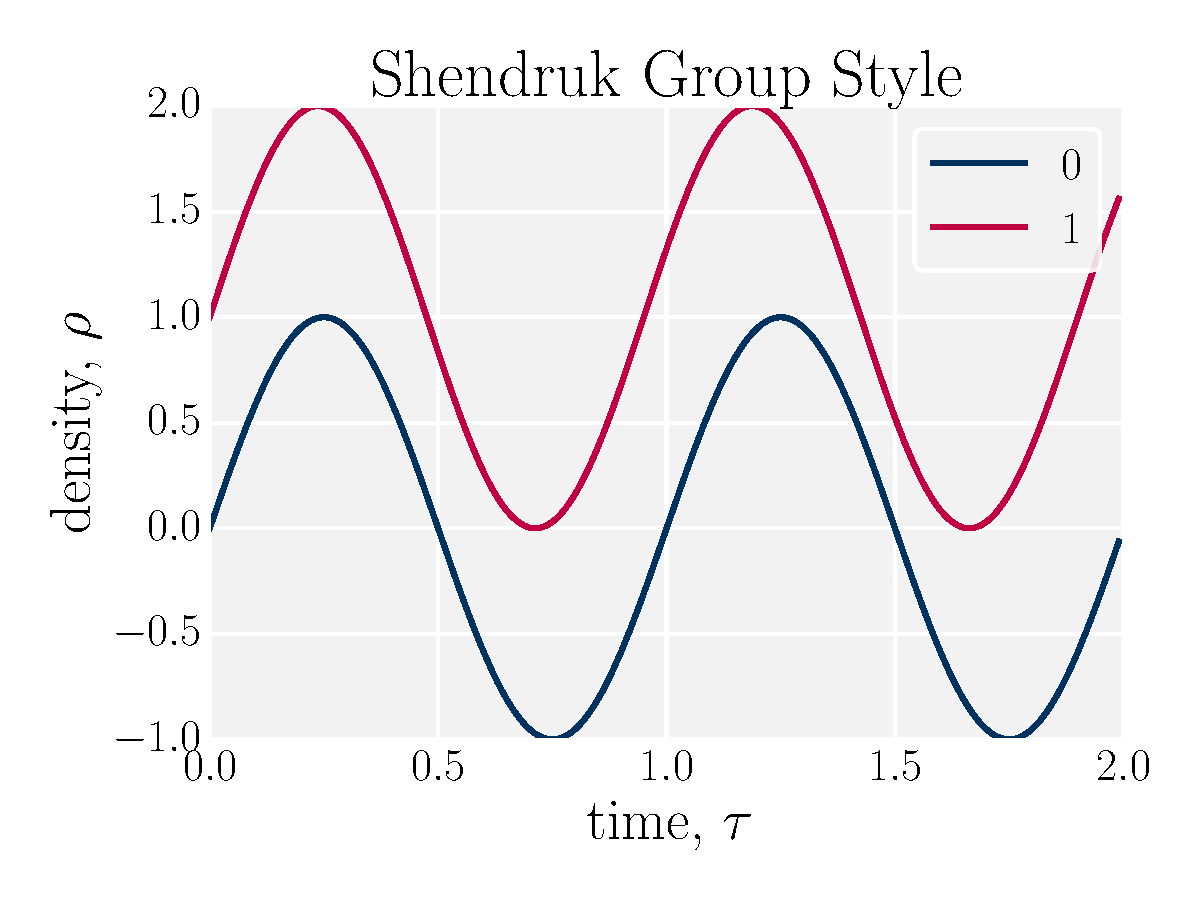
\includegraphics[width=0.45\textwidth]{linestyle.pdf}
  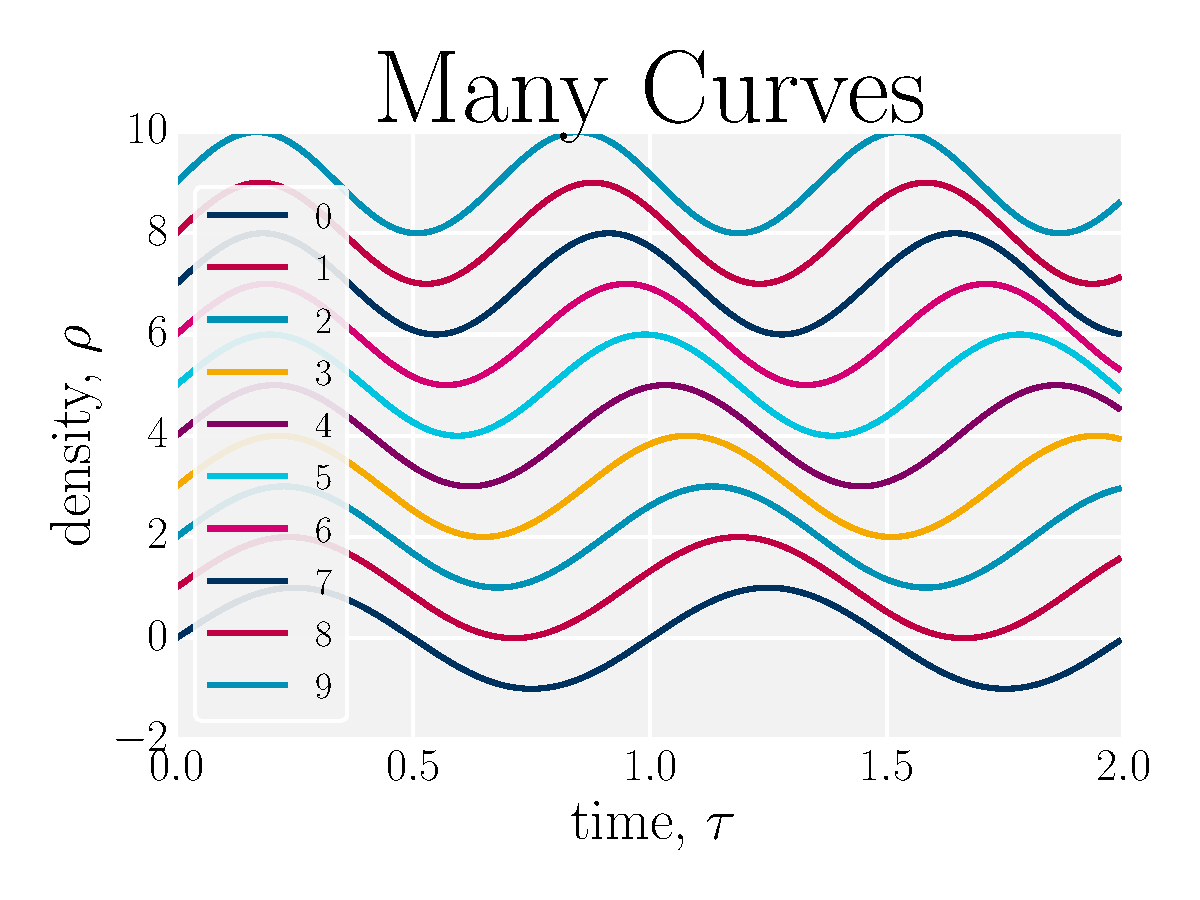
\includegraphics[width=0.45\textwidth]{manylines.pdf}
  \caption{Default plotting on left. Modified title and legend size on right.}
\end{figure}

The colours correspond to the colours Edinburgh brand colours. 
I have included seven new `default' colours that will be automatically cycled through by matplotlib. 
This is shown in the second panel with many curves. 
As before, one can override the default and change any of the options. 
For instance here, I made a legend with a frame and a white background (rather than the default of no frame and transparent background) because there are so many curves. 
To further illustrate, I increased the title-font size too. 
Colours, font size, everything can still be changed in the normal ways. 
\begin{table}[h]
  \centering
  \begin{tabular}{| l | l |}
    \hline
    \multicolumn{2}{|c|}
      {Cyclic Colours} \\
    \hline\hline
    Name & R, G, B\\ \hline
    \textbf{\color{saphire}saphire} & \textbf{\color{saphire}0, 50, 95} \\ \hline
    \textbf{\color{crimson}crimson} & \textbf{\color{crimson}193, 0, 67} \\ \hline
    \textbf{\color{capri}capri} & \textbf{\color{capri}0, 196, 223} \\ \hline
    \textbf{\color{amber}amber} & \textbf{\color{amber}244, 170, 0} \\ \hline
    \textbf{\color{plum}plum} & \textbf{\color{plum}129, 2, 98} \\ \hline
    \textbf{\color{cerulean}cerulean} & \textbf{\color{cerulean}0, 145, 181} \\ \hline
    \textbf{\color{ruby}ruby} & \textbf{\color{ruby}212, 0, 114} \\ \hline
  \end{tabular}
  \caption{The seven cyclic colours from the official Edinburgh brand included in the \texttt{shendrukGroupStyle.mplstyle} and \texttt{shendrukGroupFormat.py} files.}
\end{table}

\newpage

Edinburgh's brand include additional colours than those included in the cyclic colours. 
These can be found in the table below. 
\begin{table}[h]
  \centering
  \begin{tabular}{| l | l |}
    \hline
    \multicolumn{2}{|c|}
      {Other Official Colours} \\
    \hline\hline
    \textbf{\color{cardinal}cardinal} & \textbf{\color{cardinal}172, 0, 64} \\ \hline
    \textbf{\color{cinnamon}cinnamon} & \textbf{\color{cinnamon}205, 90, 19} \\ \hline
    \textbf{\color{limegreen}limegreen} & \textbf{\color{limegreen}41, 188, 41} \\ \hline
    \textbf{\color{gold}gold} & \textbf{\color{gold}141, 116, 74} \\ \hline
    \textbf{\color{taupe}taupe} & \textbf{\color{taupe}110, 80, 72} \\ \hline
    \textbf{\color{teal}teal} & \textbf{\color{teal}69, 126, 129} \\ \hline
    \textbf{\color{forestgreen}forestgreen} & \textbf{\color{forestgreen}0, 70, 49} \\ \hline
    \textbf{\color{mahogany}mahogany} & \textbf{\color{mahogany}106, 51, 40} \\ \hline
    \textbf{\color{silver}silver} & \textbf{\color{silver}194, 211, 223} \\ \hline
    \textbf{\color{oldrose}oldrose} & \textbf{\color{oldrose}184, 133, 141} \\ \hline
    \textbf{\color{curry}curry} & \textbf{\color{curry}156, 154, 0} \\ \hline
    \textbf{\color{cobalt}cobalt} & \textbf{\color{cobalt}0, 80, 114} \\ \hline
  \end{tabular}
  \caption{The non-cyclic colours from the official Edinburgh brand included in \texttt{shendrukGroupFormat.py} files.}
\end{table}

Finally, I also made a few modified colours (which I found useful in creating colourmaps; see below). 
\begin{table}[h]
  \centering
  \begin{tabular}{| l | l |}
    \hline
    \multicolumn{2}{|c|}
      {Modified Colours} \\
    \hline\hline
    \textbf{\color{rubydarker}rubydarker} & \textbf{\color{rubydarker}197, 0, 99} \\ \hline
    \textbf{\color{purple}purple} & \textbf{\color{purple}56, 6, 92} \\ \hline
    \textbf{\color{cardinaldarker}cardinaldarker} & \textbf{\color{cardinaldarker}97, 0, 36} \\ \hline
    \textbf{\color{ceruleandarker}ceruleandarker} & \textbf{\color{ceruleandarker}0, 113, 140} \\ \hline
    \textbf{\color{amberlighter}amberlighter} & \textbf{\color{amberlighter}240, 191, 79} \\ \hline
    \textbf{\color{amberbrighter}amberbrighter} & \textbf{\color{amberbrighter}245, 242, 88} \\ \hline
    white & 255, 255, 255 \\ \hline
    \textbf{\color{onyx}onyx} & \textbf{\color{onyx}15, 15, 15} \\ \hline
    \textbf{\color{bggrey}bggrey} & \textbf{\color{bggrey}245, 245, 245} \\ \hline
  \end{tabular}
  \caption{The modified colours in \texttt{shendrukGroupFormat.py} files.}
\end{table}

To make these conveniently accessible, I've put these into a python file called \texttt{shendrukGroupFormat.py} that can be imported. 
Not only can we access any of the colours (to use in plots \textit{etc.} but there are convenient \texttt{classes} and \texttt{functions}. 
All codes import set the group style and import the group format file:
\begin{lstlisting}[language=Python]
import numpy as np
import matplotlib.pyplot as plt
plt.style.use('shendrukGroupStyle')
import shendrukGroupFormat as ed
\end{lstlisting}


As an example of how to use the imported \texttt{shendrukGroupFormat.py} file, the following code imports the it as \texttt{ed} and then prints the RGB for saphire then uses the list of colours (\texttt{clist()}) to print all the cyclic colours and finally prints the RGB for saphire again from the list of cyclic colours. 
\begin{lstlisting}[language=Python]
print ed.saphire
print ed.clist().cyclic
print ed.clist().cyclic["saphire"]
\end{lstlisting}
The output is
\begin{verbatim}
 [0, 0.19607843137254902, 0.37254901960784315]
 {'amber': [0.9568627450980393, 0.6666666666666666, 0], 
 'plum': [0.5058823529411764, 0.00784313725490196, 0.3843137254901961], 
 'capri': [0, 0.7686274509803922, 0.8745098039215686], 
 'cerulean': [0, 0.5686274509803921, 0.7098039215686275], 
 'crimson': [0.7568627450980392, 0, 0.2627450980392157], 
 'saphire': [0, 0.19607843137254902, 0.37254901960784315], 
 'ruby': [0.8313725490196079, 0, 0.4470588235294118]}
 [0, 0.19607843137254902, 0.37254901960784315]
\end{verbatim}
This can be done for any of the lists \textit{i.e.}
\begin{lstlisting}[language=Python]
print ed.clist().cyclic
print ed.clist().noncyclic
print ed.clist().modified
print ed.clist().official
print ed.clist().all
\end{lstlisting}

If you forget what these colours look like, \texttt{shendrukGroupFormat.py} contains a convenient table maker, called \texttt{plot\_colortable()}. 
The following code will make five colourtables. 
\begin{lstlisting}[language=Python]
ed.plot_colortable(ed.clist().cyclic, "Cyclic" )
ed.plot_colortable(ed.clist().noncyclic, "Noncyclic" )
ed.plot_colortable(ed.clist().modified, "Modified" )
ed.plot_colortable(ed.clist().official, "Official" )
ed.plot_colortable(ed.clist().all, "All" )
plt.show()
\end{lstlisting}
\begin{figure}[h]
  \centering
  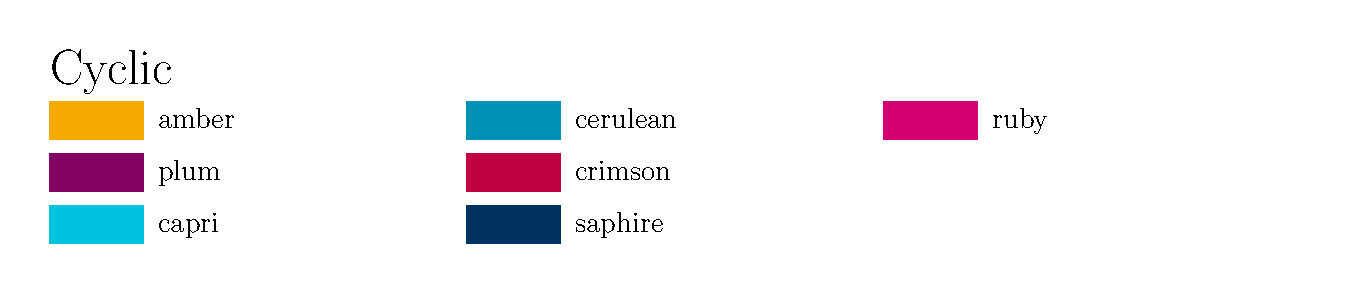
\includegraphics[width=0.45\textwidth]{tableCyclic.pdf}
  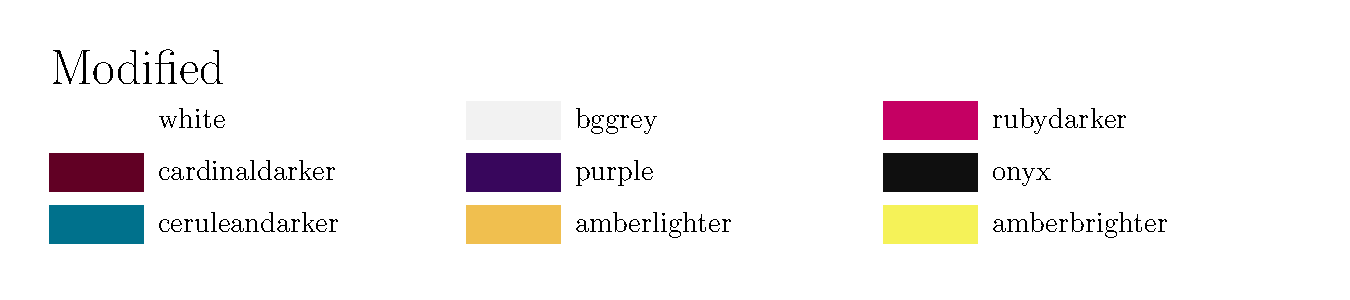
\includegraphics[width=0.45\textwidth]{tableModified.pdf}\\
  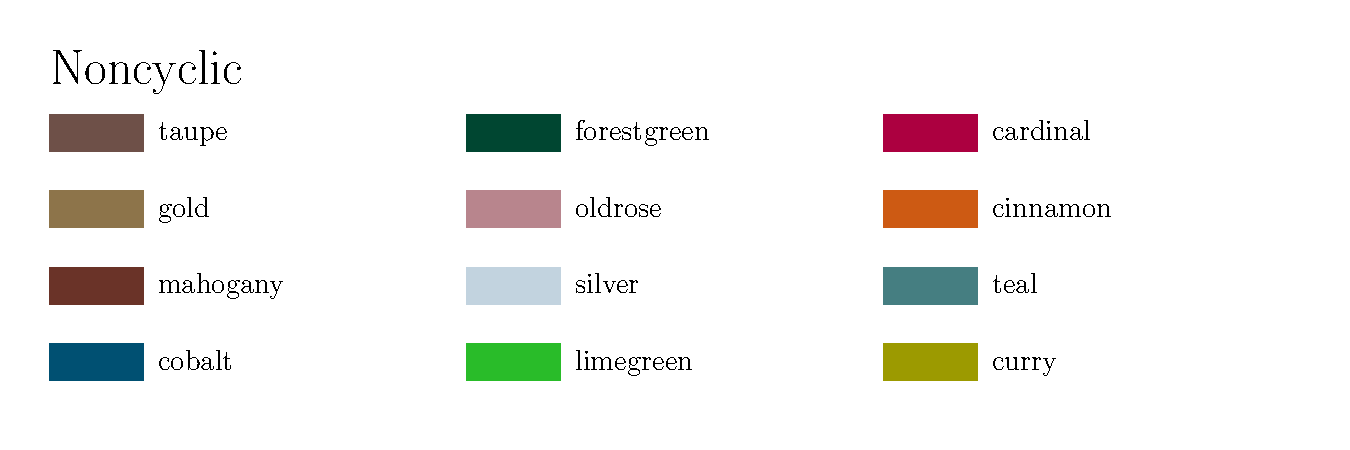
\includegraphics[width=0.45\textwidth]{tableNoncyclic.pdf}\\
  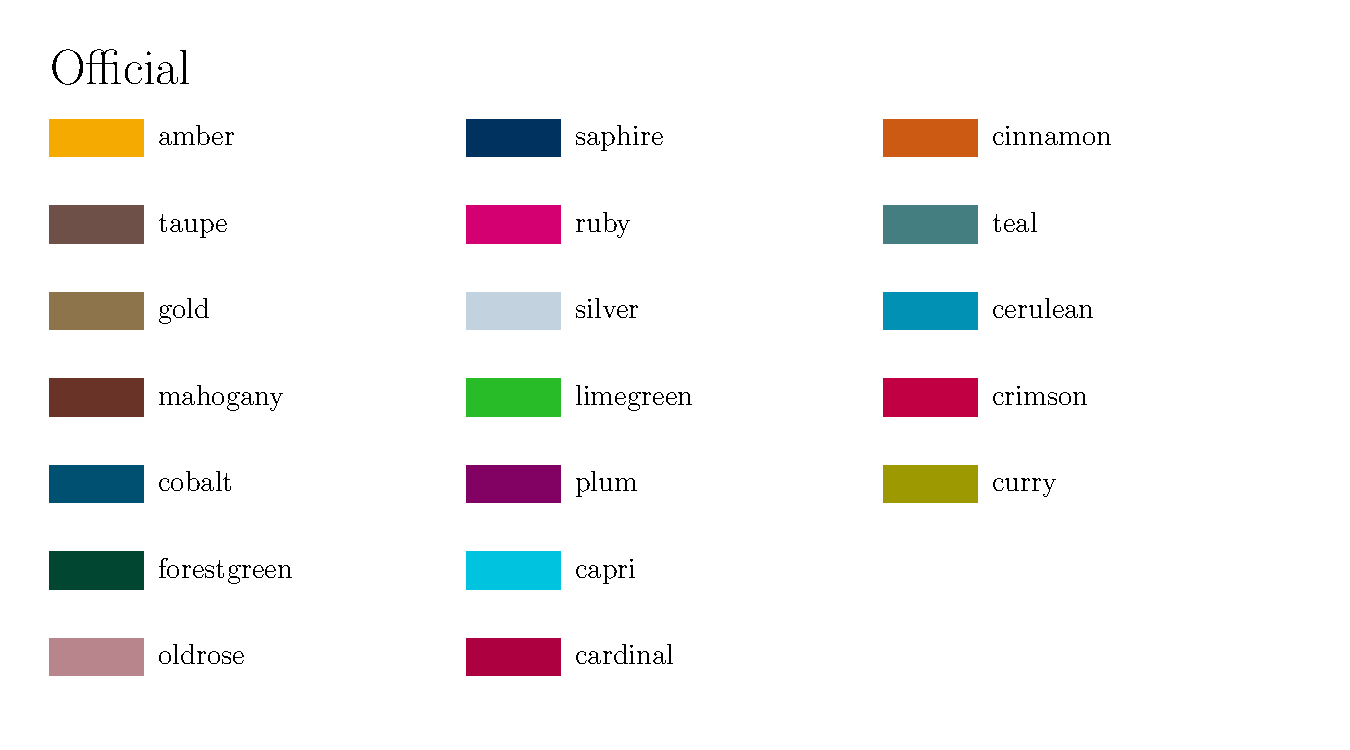
\includegraphics[width=0.45\textwidth]{tableOfficial.pdf}
  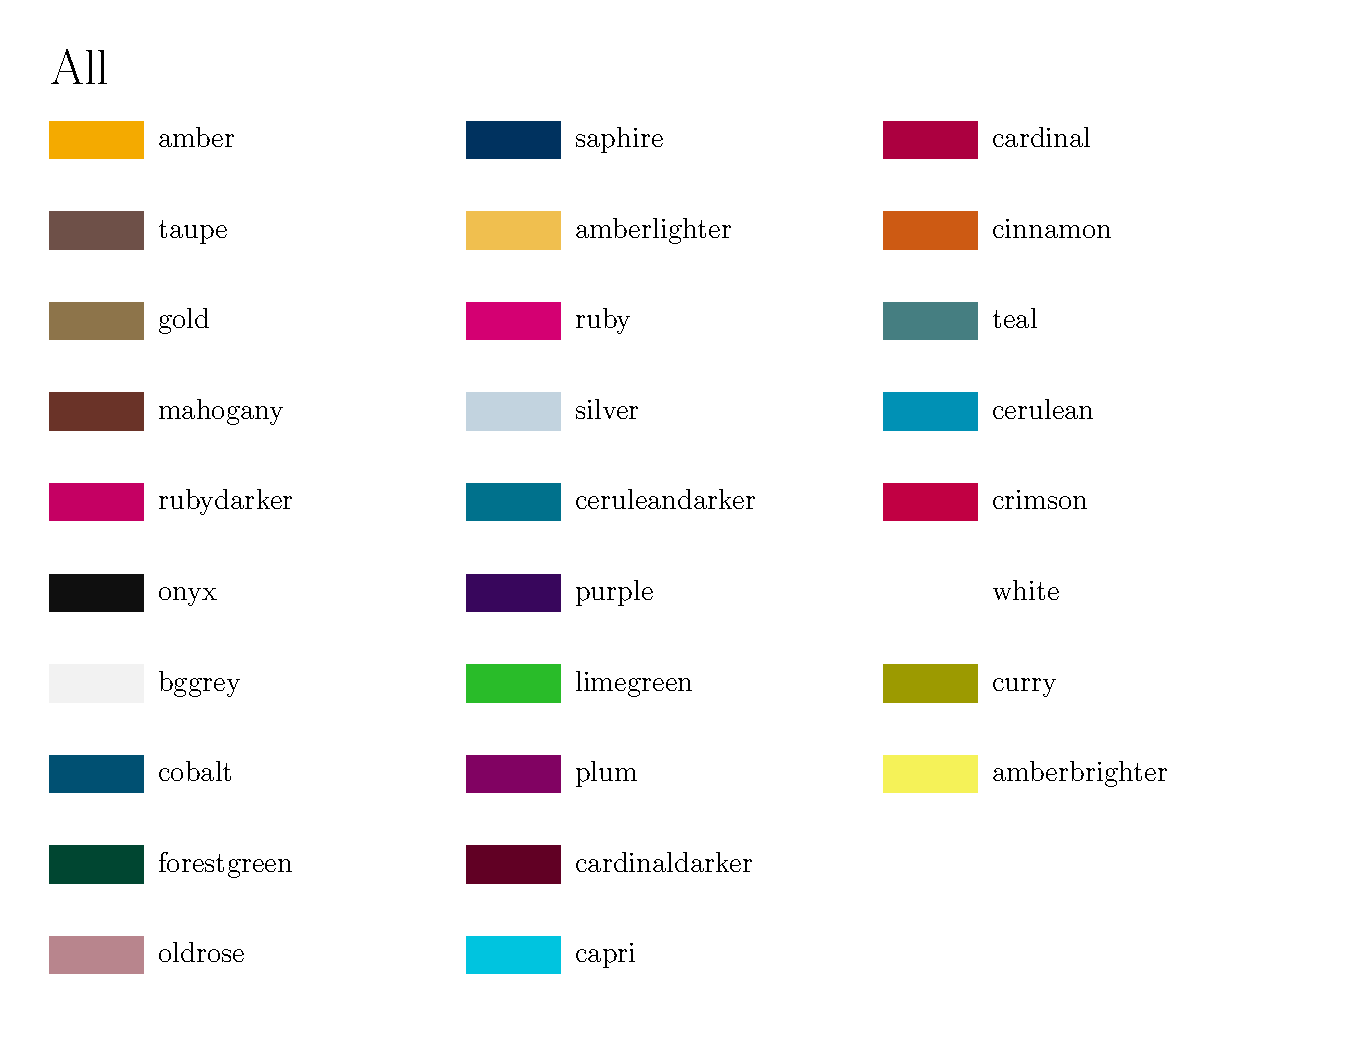
\includegraphics[width=0.45\textwidth]{tableAll.pdf}
  \caption{Colour tables produced by \texttt{plot\_colortable()} in \texttt{shendrukGroupFormat.py}.}
\end{figure}
If one wants to plot using colours or groups of colours from \texttt{shendrukGroupFormat.py} instead of just the automantic cyclic colours, this should now be convenient. 

\newpage

I'll quick put up a few examples of this style will look for other types of graphs.

\begin{lstlisting}[language=Python]
N = 10
for i in ed.clist().official:
    x = np.random.rand(N)
    y = np.random.rand(N)
    colors = np.random.rand(N)
    area = np.pi * (15 * np.random.rand(N))**2
    plt.scatter(x, y, s=area, c=ed.clist().official[i], alpha=0.75, label=i)
\end{lstlisting}
\begin{figure}[h]
  \centering
  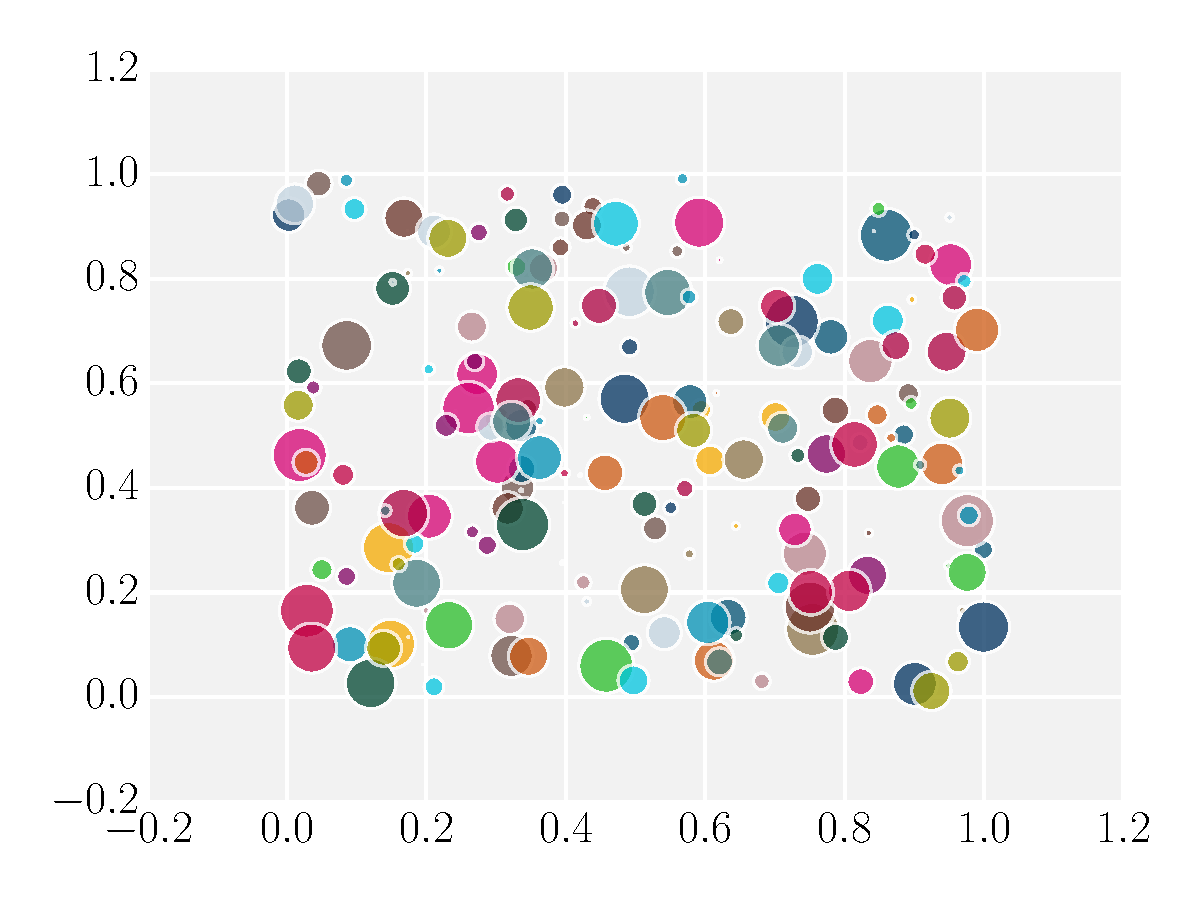
\includegraphics[width=0.45\textwidth]{scatter.pdf}
  \caption{Scatter plot. Notice that scatter plots \textbf{do not} cycle so the user must specify colours.}
\end{figure}

\begin{lstlisting}[language=Python]
x = np.arange(0.1, 4, 0.5)
y = np.exp(-x)
y2 = 1.0-np.exp(-x)
y2err=0.2*y
fig, ax = plt.subplots()
ax.errorbar(x, y, xerr=0.2, yerr=0.4, marker='o')
ax.errorbar(x, y2, yerr=y2err)
ax.errorbar(x, y2-y, yerr=0.4, marker='s')
fig, ax = plt.subplots()
ed.errorbar_fill(x,y,yerr=0.4,marker='o')
ed.errorbar_fill(x,y2,yerr=y2err)
ed.errorbar_fill(x,y2-y,yerr=0.4,marker='s')
\end{lstlisting}
\begin{figure}[h]
  \centering
  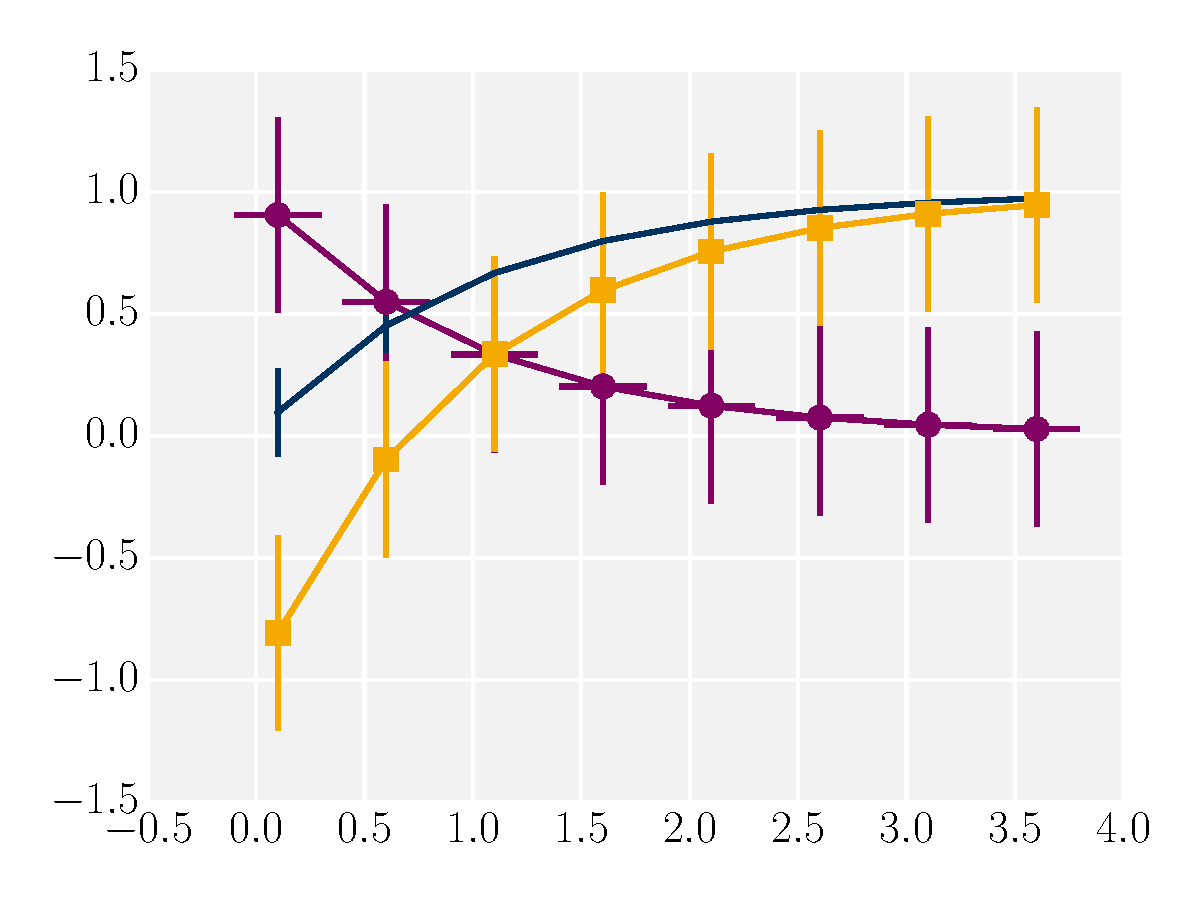
\includegraphics[width=0.4\textwidth]{errorbar.pdf}
  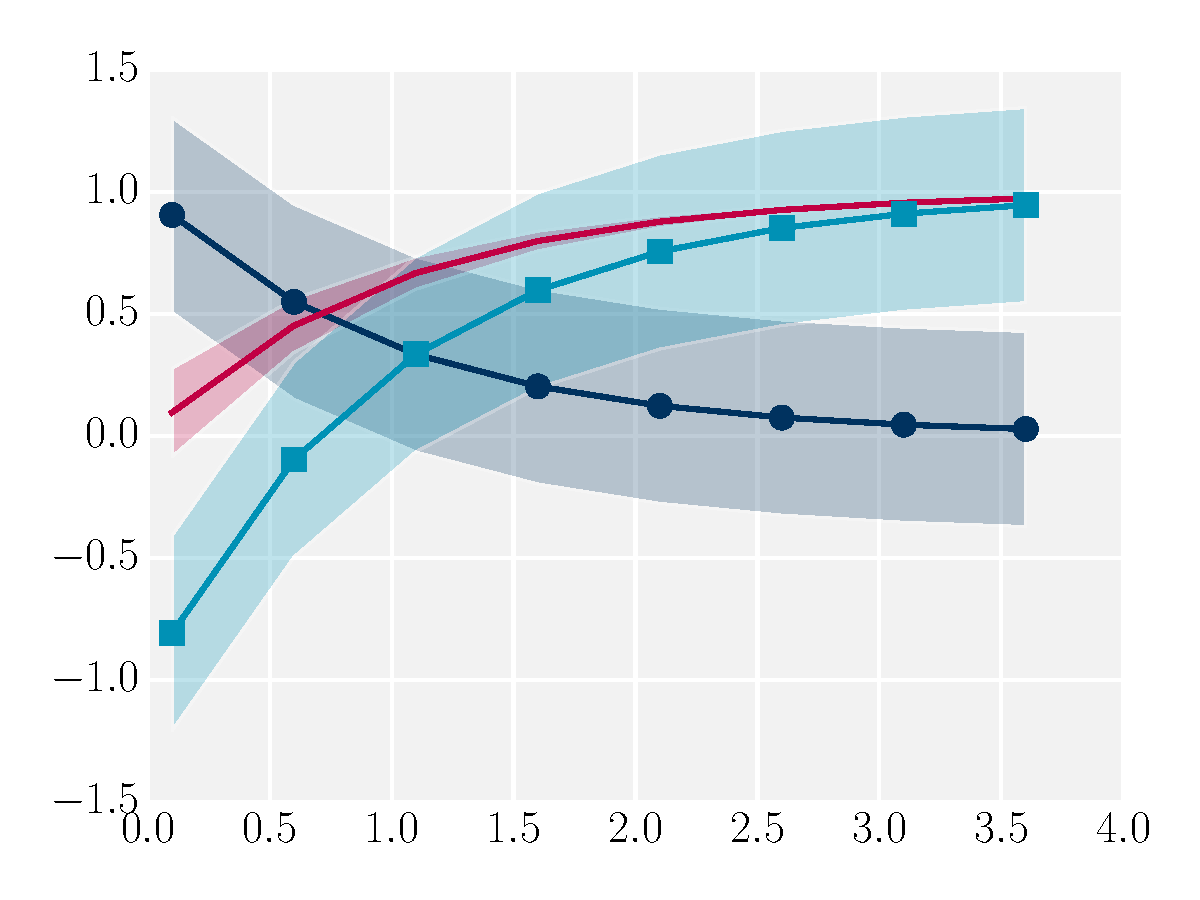
\includegraphics[width=0.4\textwidth]{errorfill.pdf}
  \caption{On the left is the default errorbars using the \texttt{shendrukGroupFormat} and \texttt{shendrukGroupStyle}. On the right, showing the error as a fill between points, which I find far more elegent when we have lots and lots of data points as frequently occurs (I like this better even with fewer).}
\end{figure}

\newpage

\begin{lstlisting}[language=Python]
np.random.seed(0)
mu = 10
sigma = 15
x = mu + sigma * np.random.randn(600)
fig, ax = plt.subplots()
n, bins, patches = ax.hist(x, 50, normed=1)
y = mlab.normpdf(bins, mu, sigma)
ax.plot(bins, y, '-o')
ax.set_ylabel('Probability density')
ax.set_title(r'$\mu=100$, $\sigma=15$')
\end{lstlisting}
\begin{figure}[h]
  \centering
  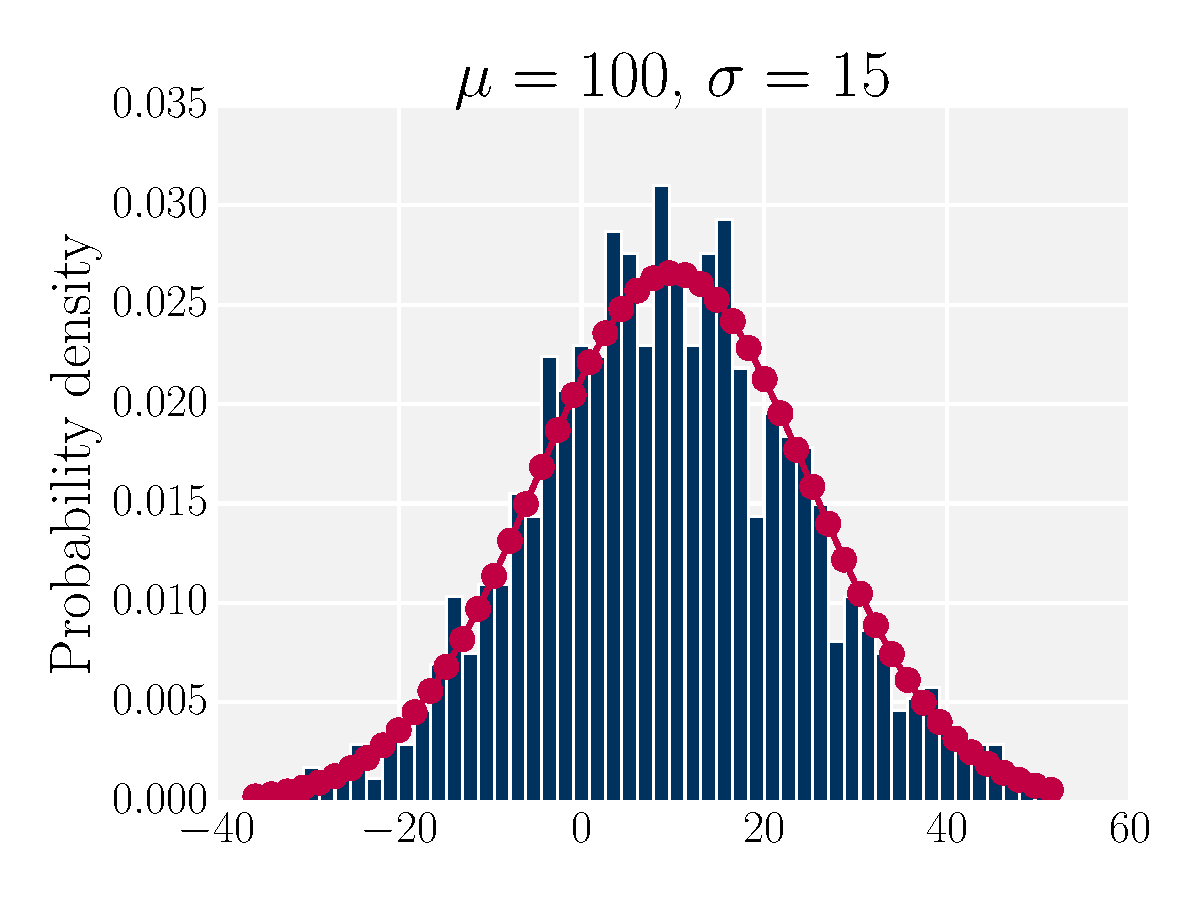
\includegraphics[width=0.5\textwidth]{hist.pdf}
  \caption{Histogram and fit.}
\end{figure}

\begin{lstlisting}[language=Python]
dt = 0.001
t = np.arange(0.0, 10.0, dt)
r = np.exp(-t[:1000]/0.05)               # impulse response
x = np.random.randn(len(t))
s = np.convolve(x, r)[:len(x)]*dt  # colored noise

# the main axes is subplot(111) by default
plt.plot(t, s)
plt.axis([0, 1, 1.1*np.amin(s), 2*np.amax(s)])
plt.xlabel('time (s)')
plt.ylabel('current (nA)')
plt.title('Gaussian colored noise')

# this is an inset axes over the main axes
inset1 = plt.axes([.7, .6, .2, .2])
inset1.patch.set_facecolor(ed.silver)
n, bins, patches = plt.hist(s, 400, normed=1,edgecolor=ed.saphire)
plt.title('Probability',fontsize=ed.fontsize)
plt.xticks([])
plt.yticks([])

# this is another inset axes over the main axes
inset2 = plt.axes([0.25, 0.6, .2, .2])
inset2.patch.set_facecolor(ed.silver)
plt.plot(t[:len(r)], r)
plt.title('Impulse',fontsize=ed.fontsize)
plt.xlim(0, 0.2)
inset2.tick_params(axis="x",labelsize=ed.fontsizeTiny)
inset2.tick_params(axis="y",labelsize=ed.fontsizeTiny)
\end{lstlisting}
\begin{figure}[h]
  \centering
  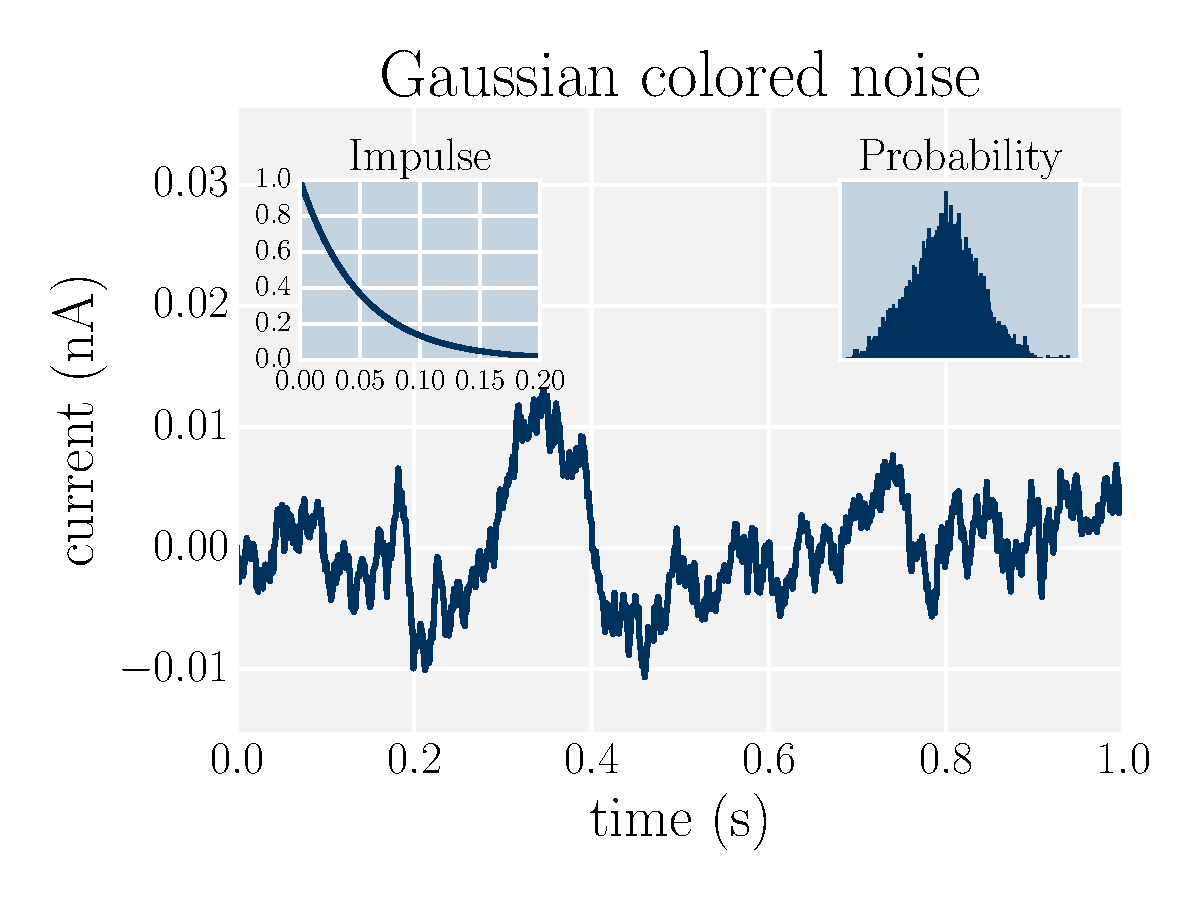
\includegraphics[width=0.45\textwidth]{insets.pdf}
  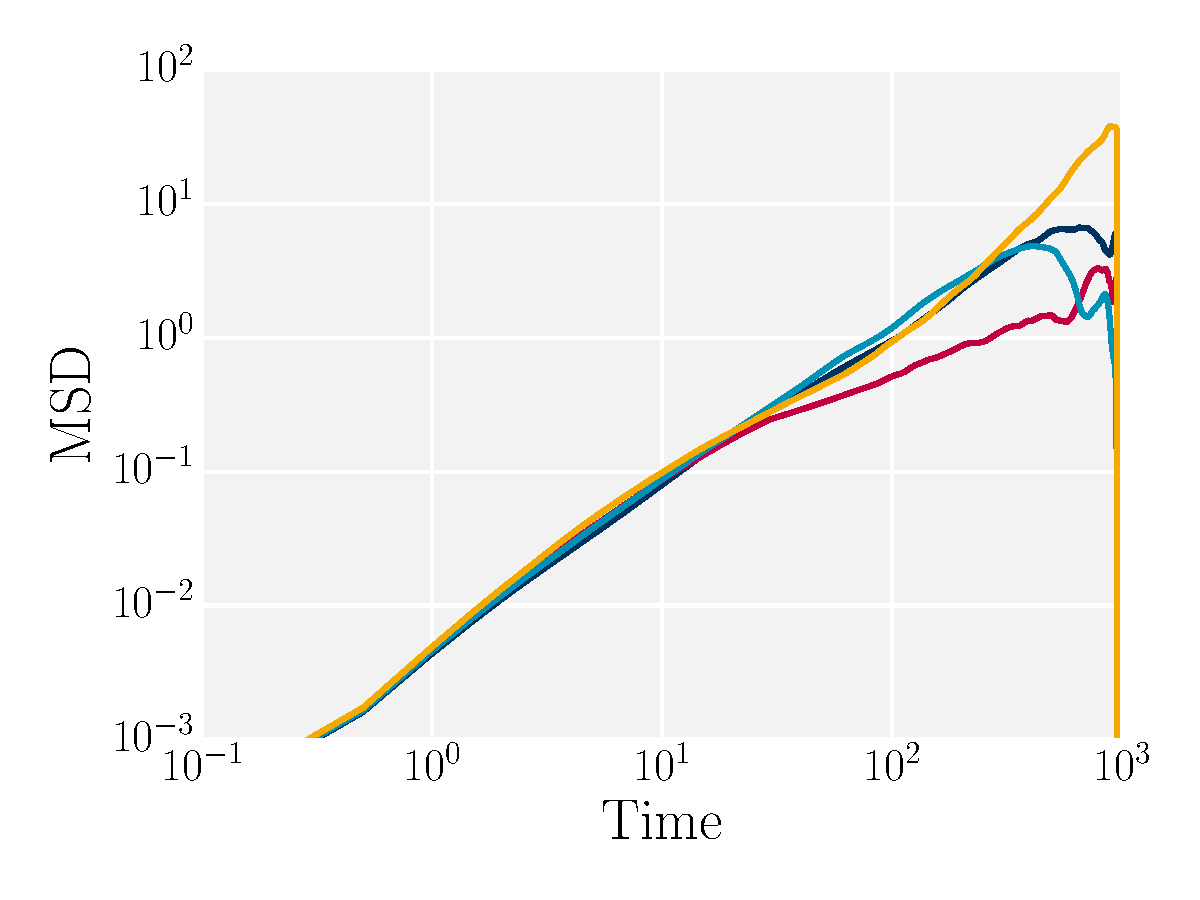
\includegraphics[width=0.5\textwidth]{loglog.pdf}
  \caption{Insets on left. A simple log-log graph on right.}
\end{figure}

In addition to setting up these individual colours, I've also created a set of colour maps. 
These colour maps are modelled after standard \texttt{matplotlib} colour maps \textbf{but} I've used the Edinburgh colours (or slight modifications) to build unique versions of the colour maps for the group. 
Hopefully, this will give our work a unified but distinct look. 

Choosing a proper colour map depends a lot on what you're doing with it --- not all of these colour maps are equally good for all purposes. 
Importantly, many colour maps can put misleading emphasis on different regions because different colours are perceived more than others. 
The previously ubiquitous colour map \texttt{jet} was infamous for this and both \texttt{matplotlib} and Matlab have removed it from being the default and replaced it with ``perceptually uniform sequential'' maps, such as  `viridis', `plasma', `inferno' and `magma'. 
However, at other times you don't want ``perceptually uniform sequential'' but rather would like ``diverging'' which goes from one dark colour through a light colour to another dark colour. 
We commonly use these for fields like vorticity. 
See \url{https://matplotlib.org/3.1.0/tutorials/colors/colormaps.html} for more information with respect to \texttt{matplotlib} colour maps. 

But I've created a set of eight for us to chose from. 
In what follows, I compare my version to the ``standard'' matplotlib version then plot six common-ish types of graphs that might use a colour map. 

% First I show the eight proposals that I suggest we keep as options (final tweaks still needed) then I'll show a few rejects in case they really appeal to either of you. 

\newpage
\begin{figure}[ht]
  \centering
  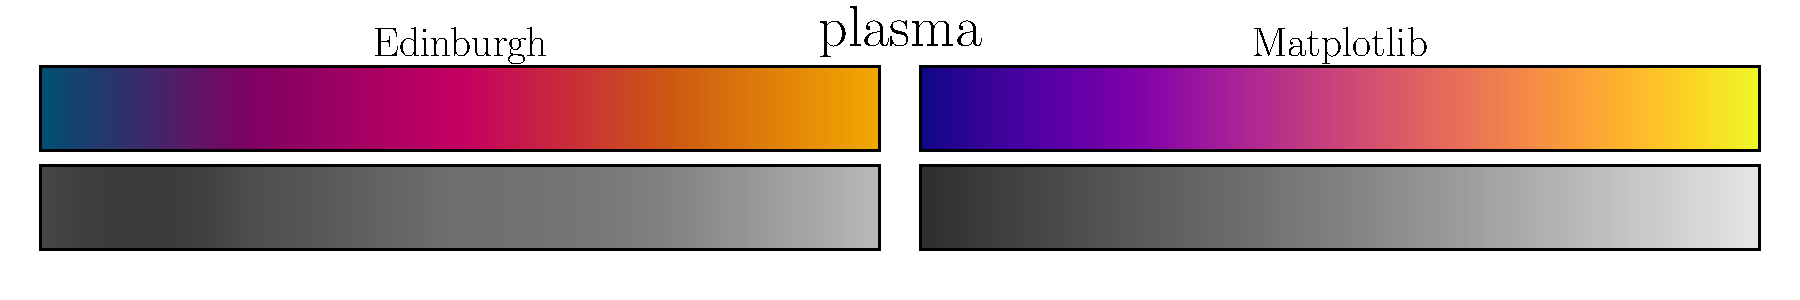
\includegraphics[width=0.99\textwidth]{plasmaBars.pdf}
  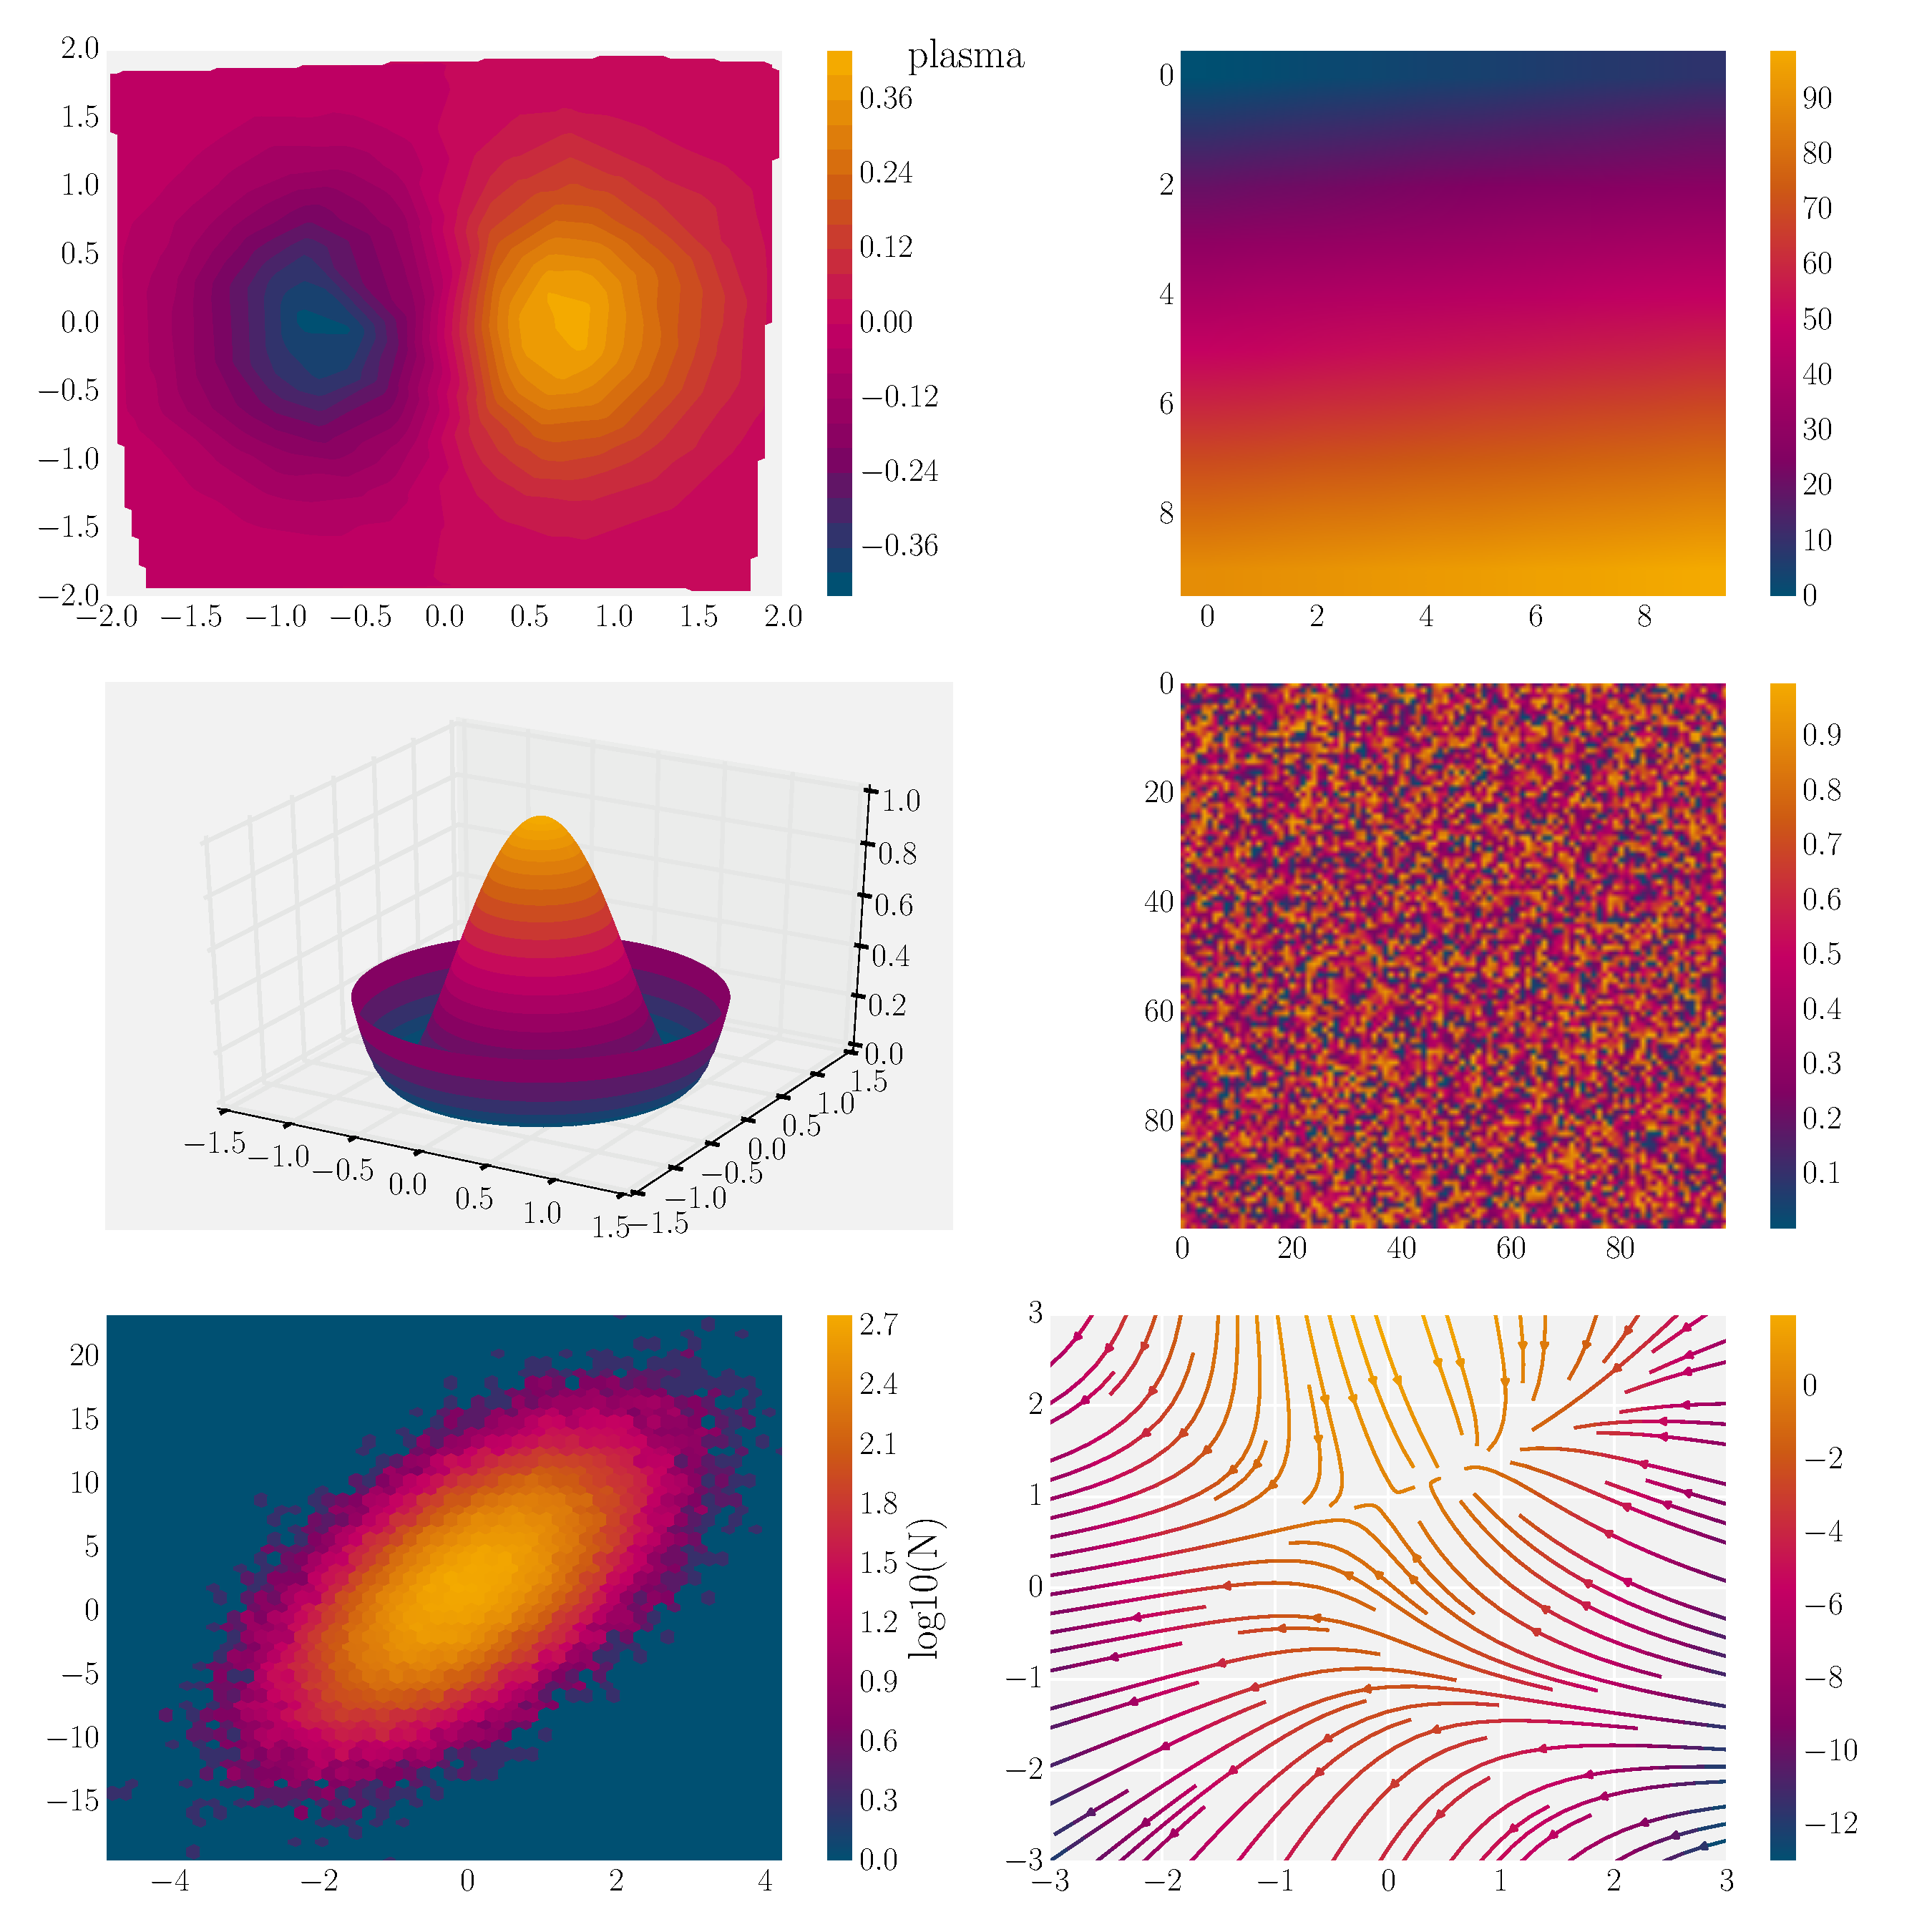
\includegraphics[width=0.99\textwidth]{plasmaExamples.pdf}
\end{figure}

\newpage
\begin{figure}[ht]
  \centering
  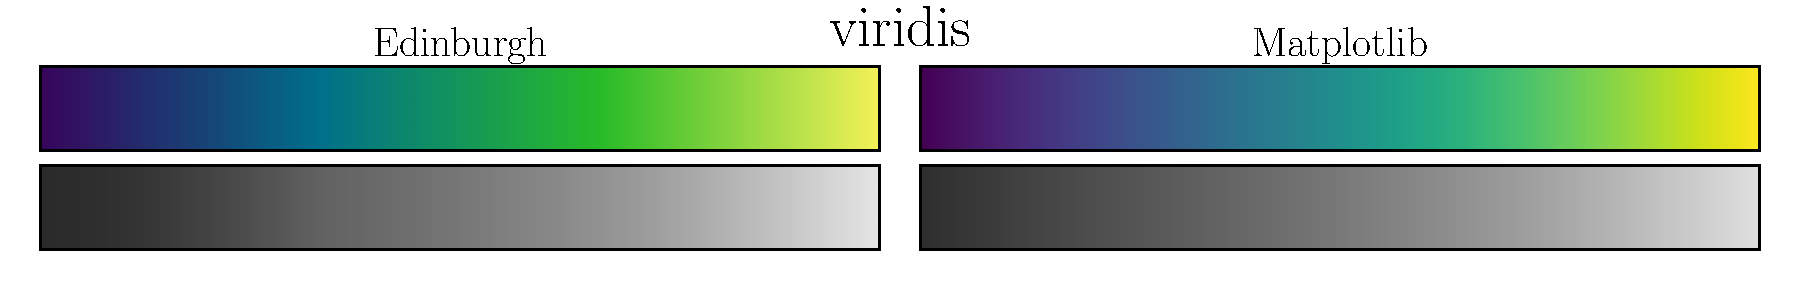
\includegraphics[width=0.99\textwidth]{viridisBars.pdf}
  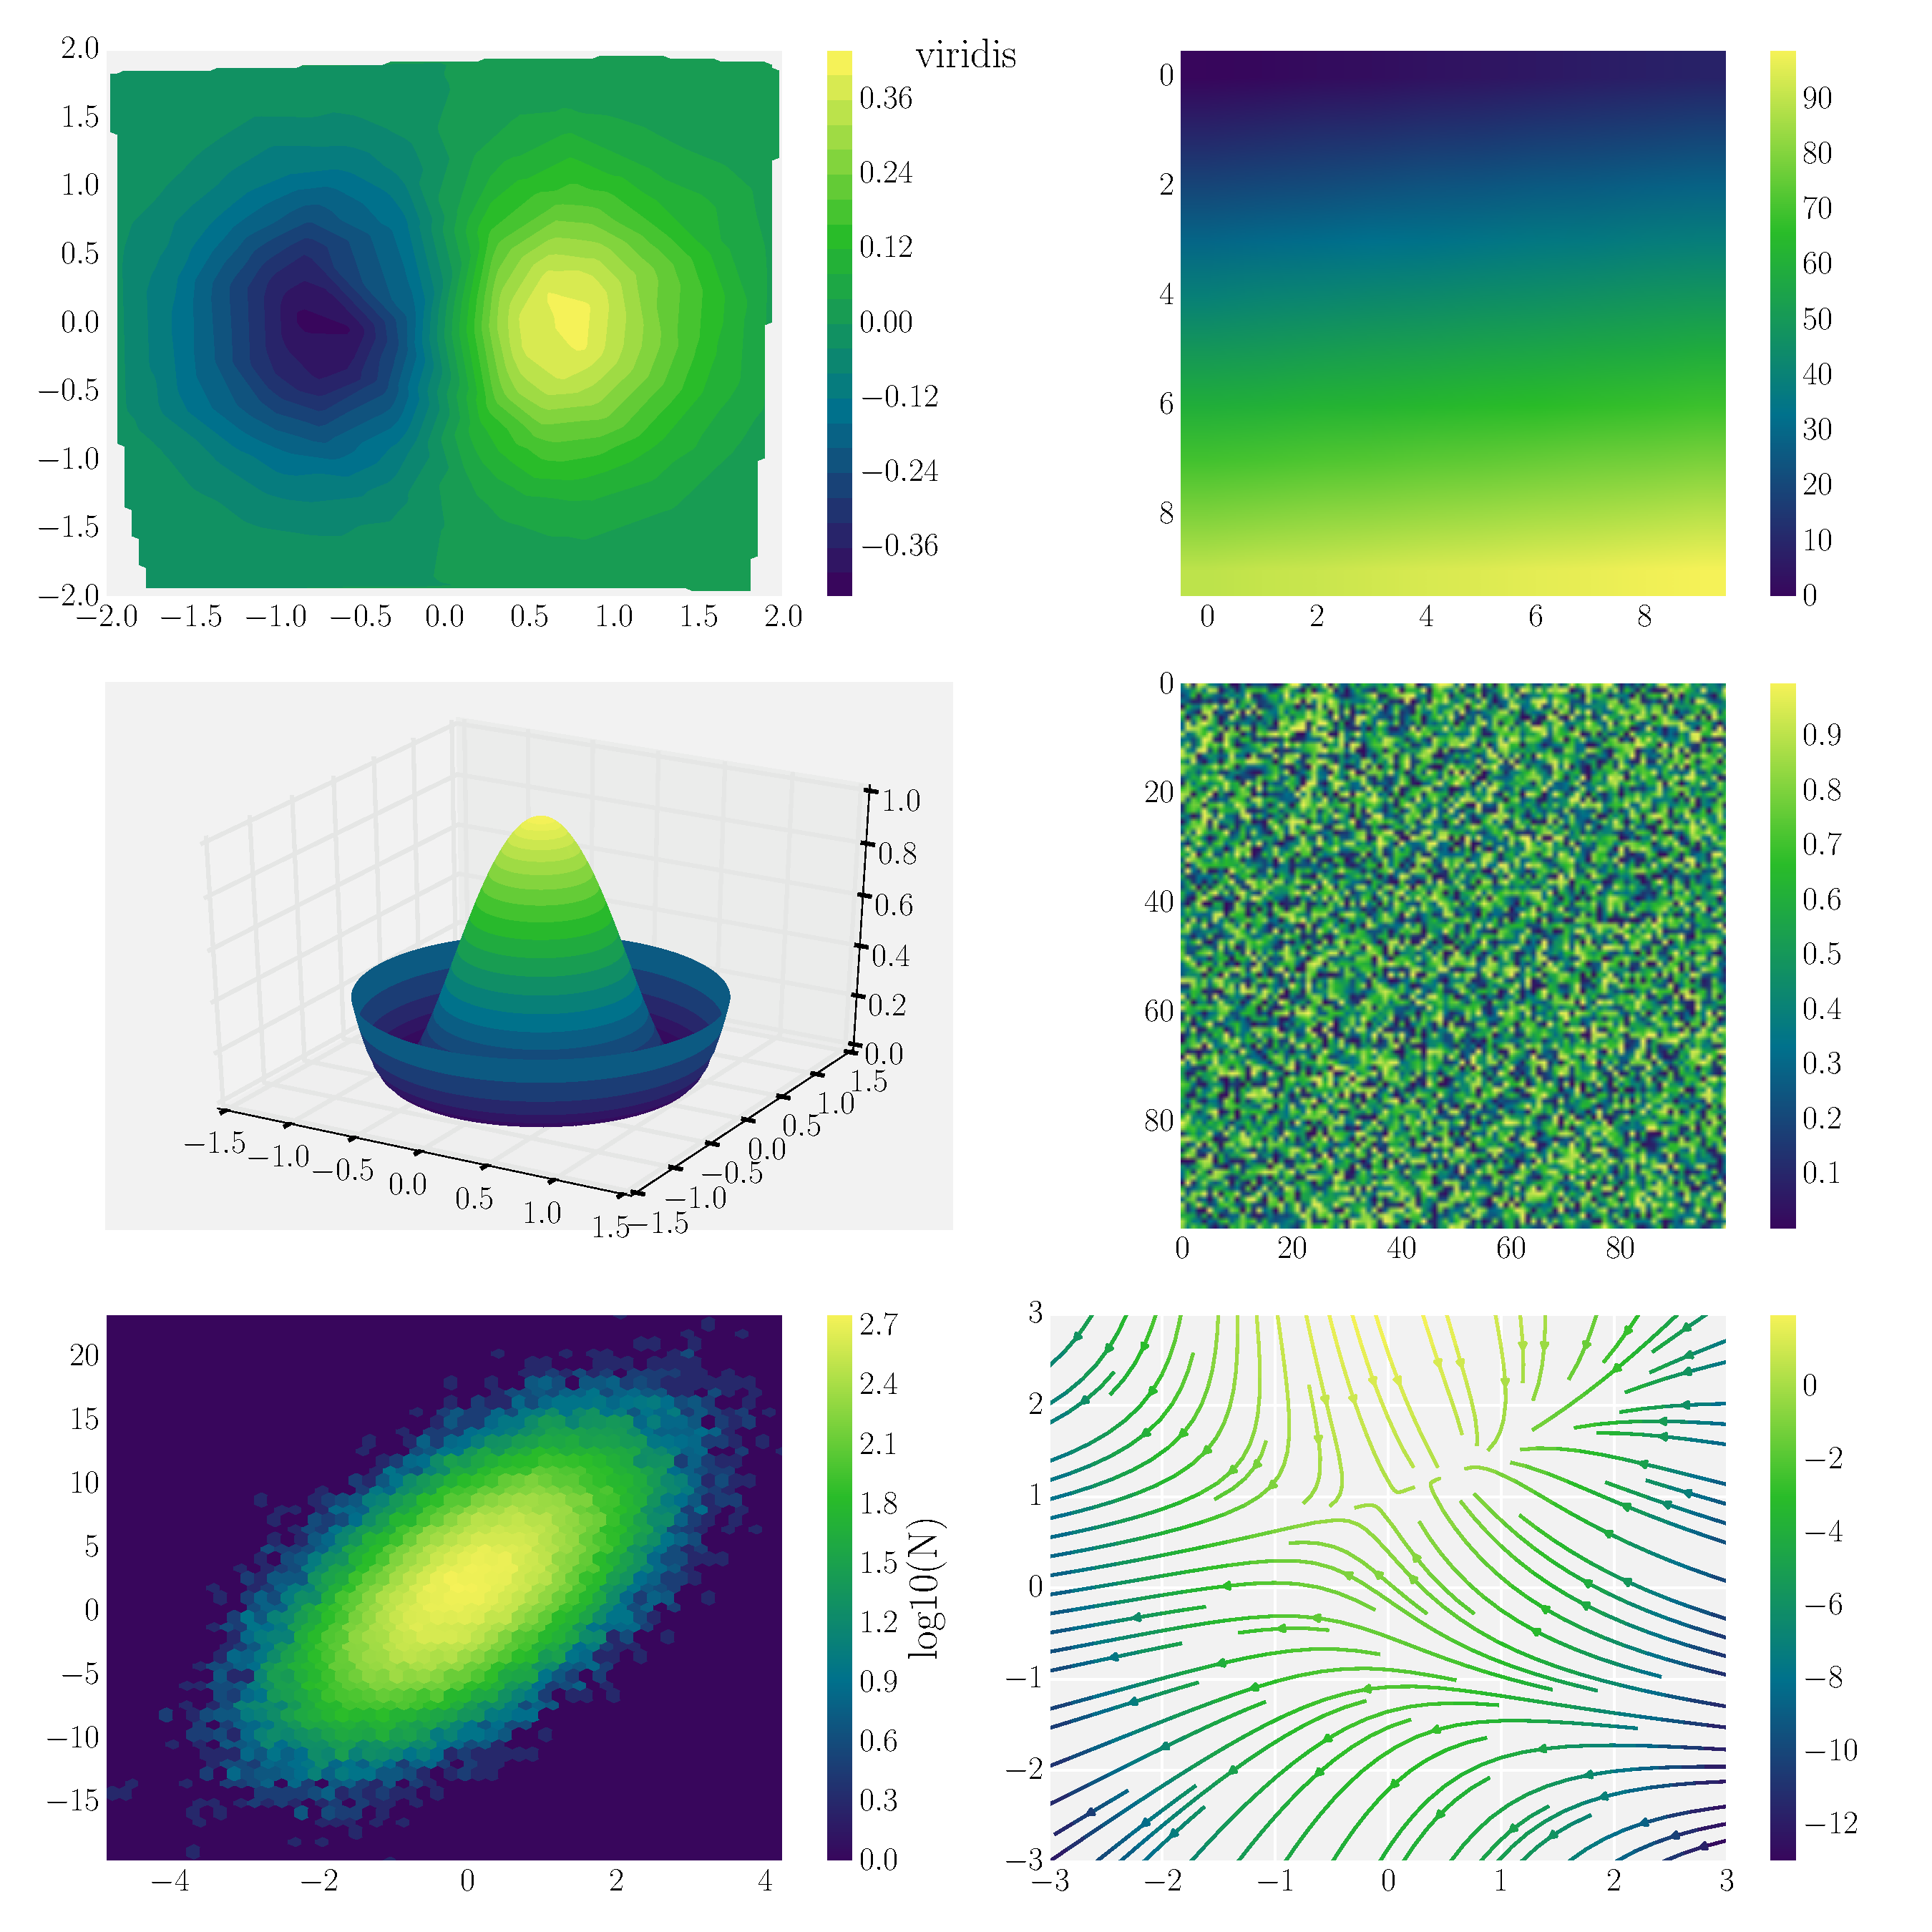
\includegraphics[width=0.99\textwidth]{viridisExamples.pdf}
\end{figure}

\newpage
\begin{figure}[ht]
  \centering
  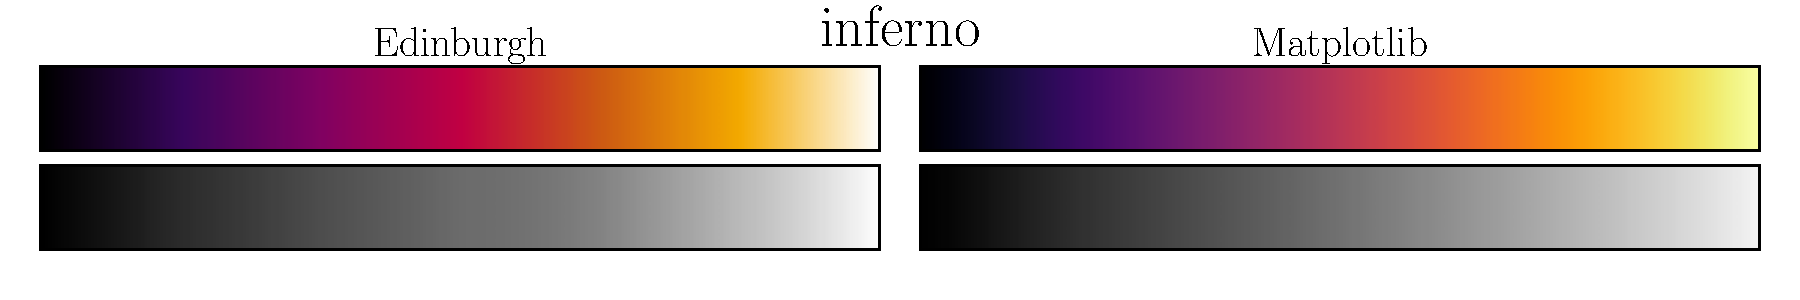
\includegraphics[width=0.99\textwidth]{infernoBars.pdf}
  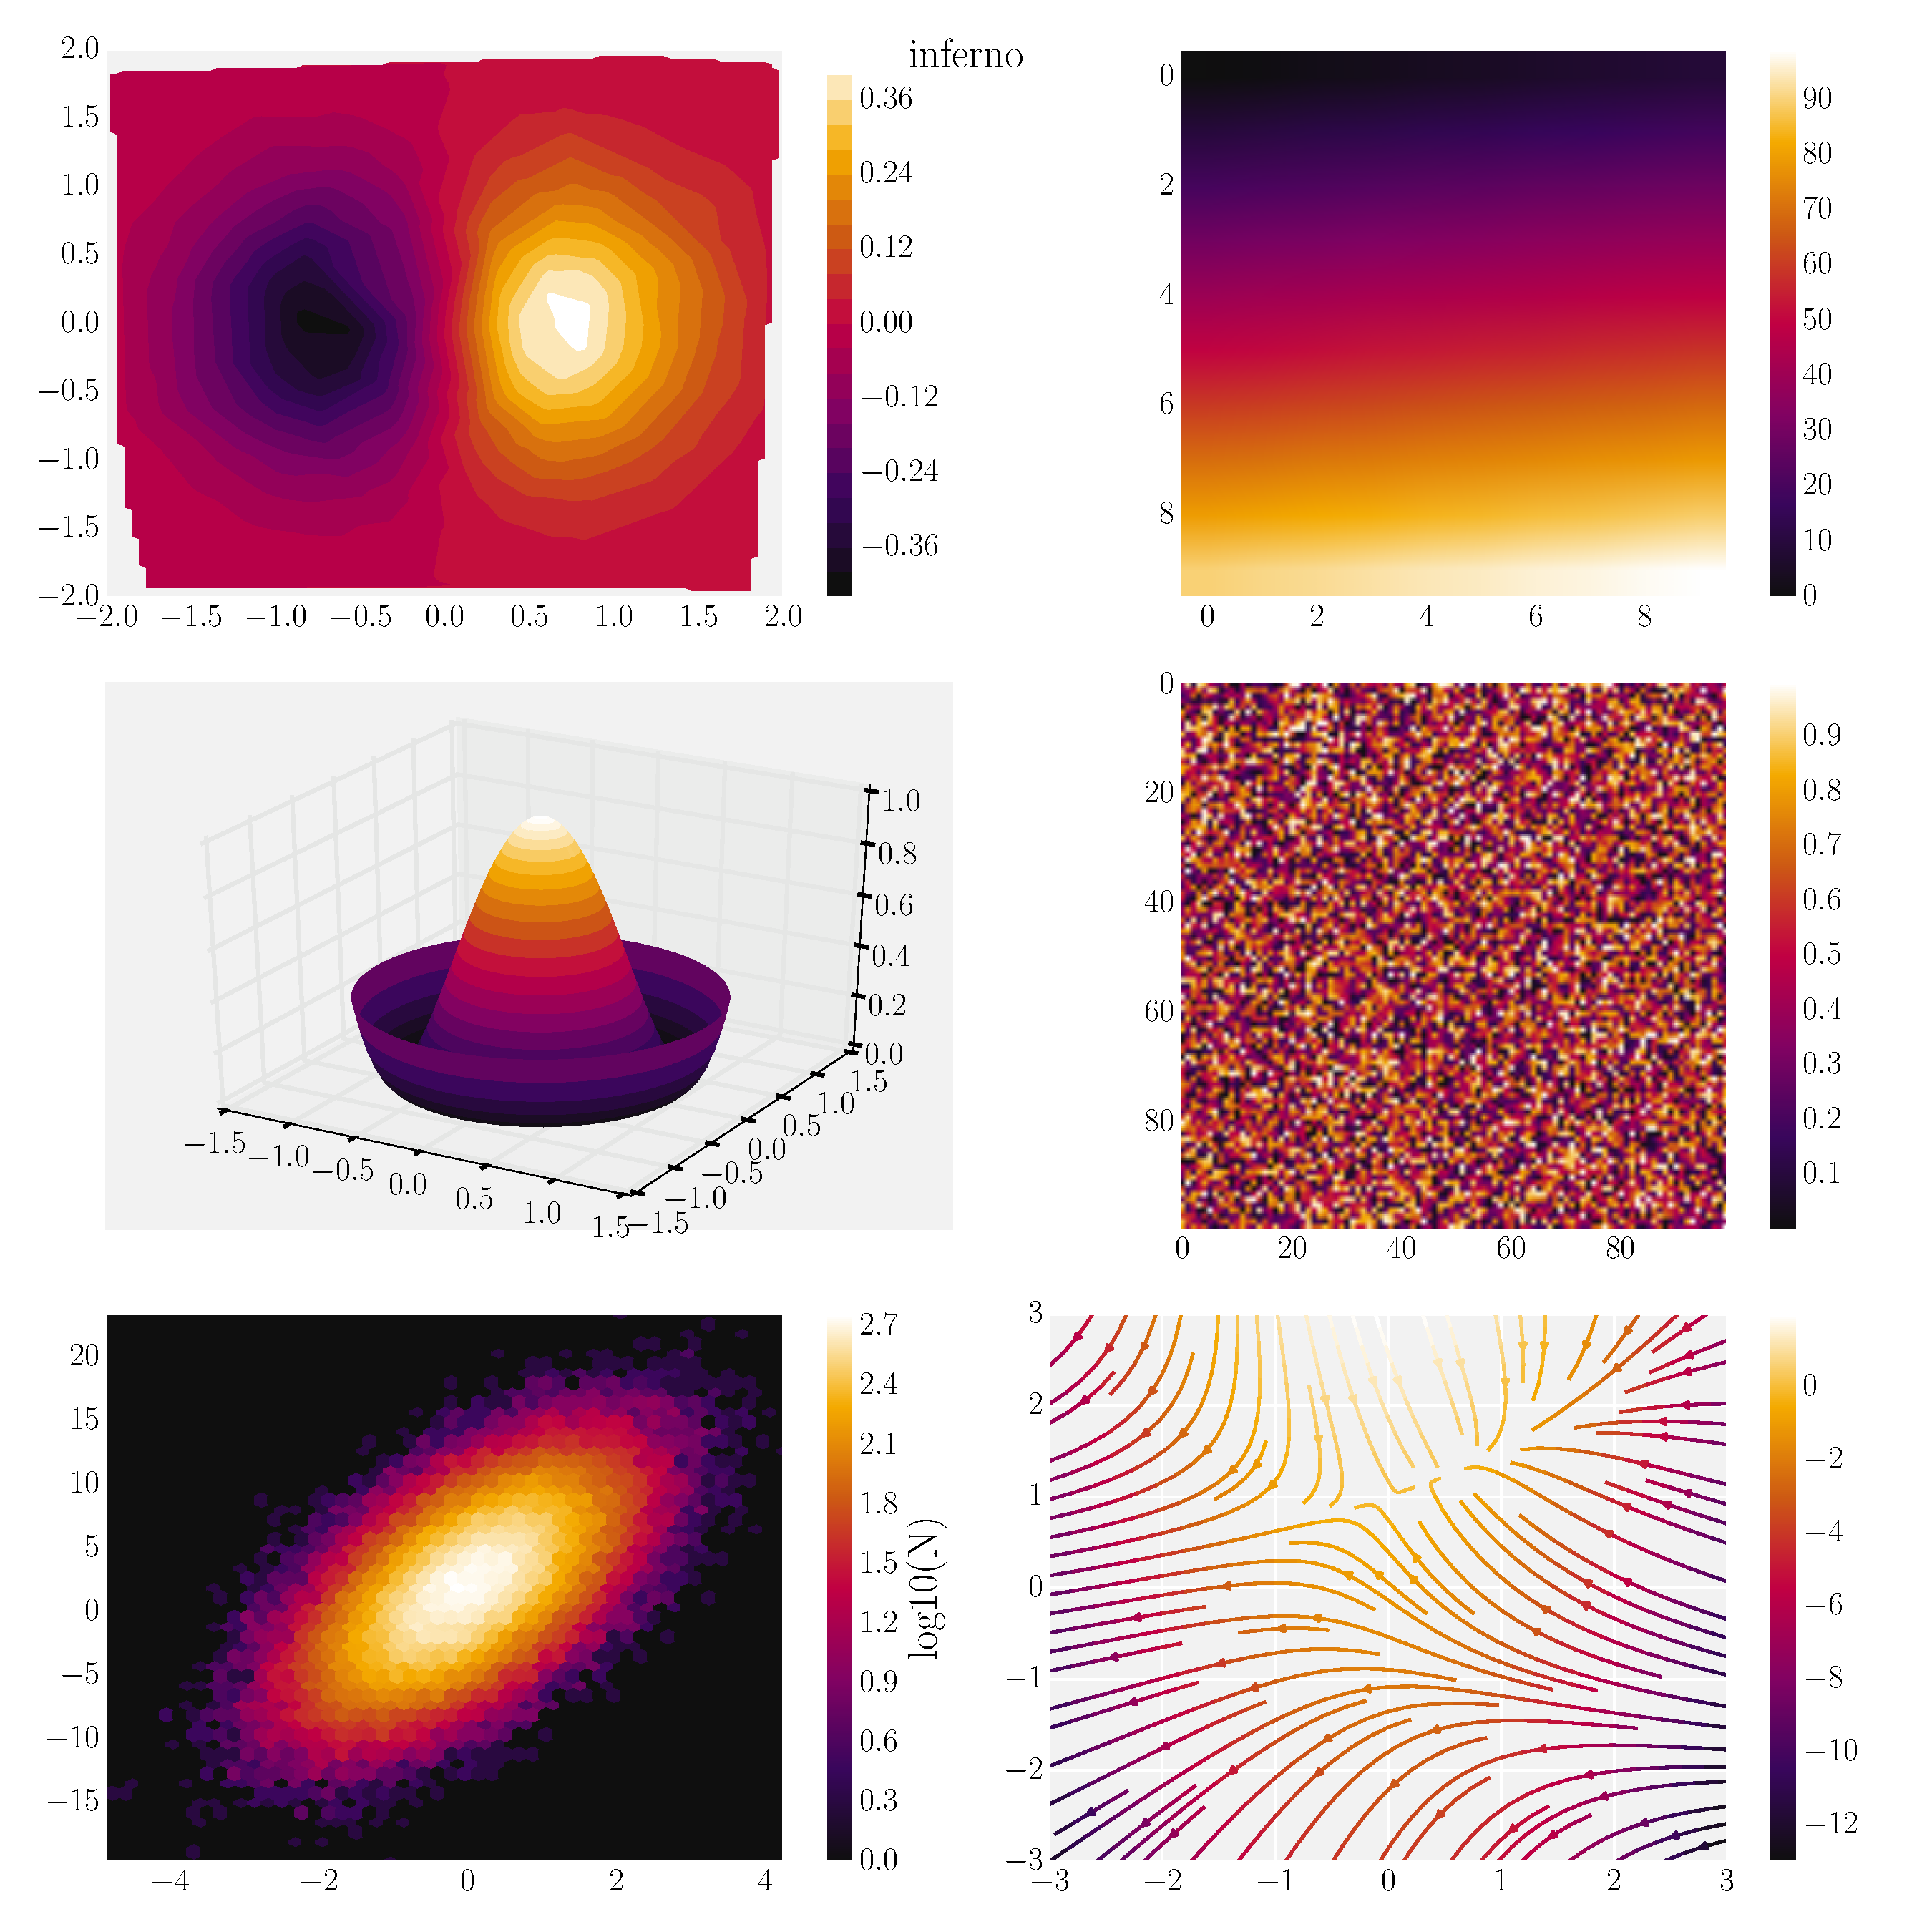
\includegraphics[width=0.99\textwidth]{infernoExamples.pdf}
\end{figure}

\newpage
\begin{figure}[ht]
  \centering
  
\includegraphics[width=0.99\textwidth]{rainBars.pdf}
  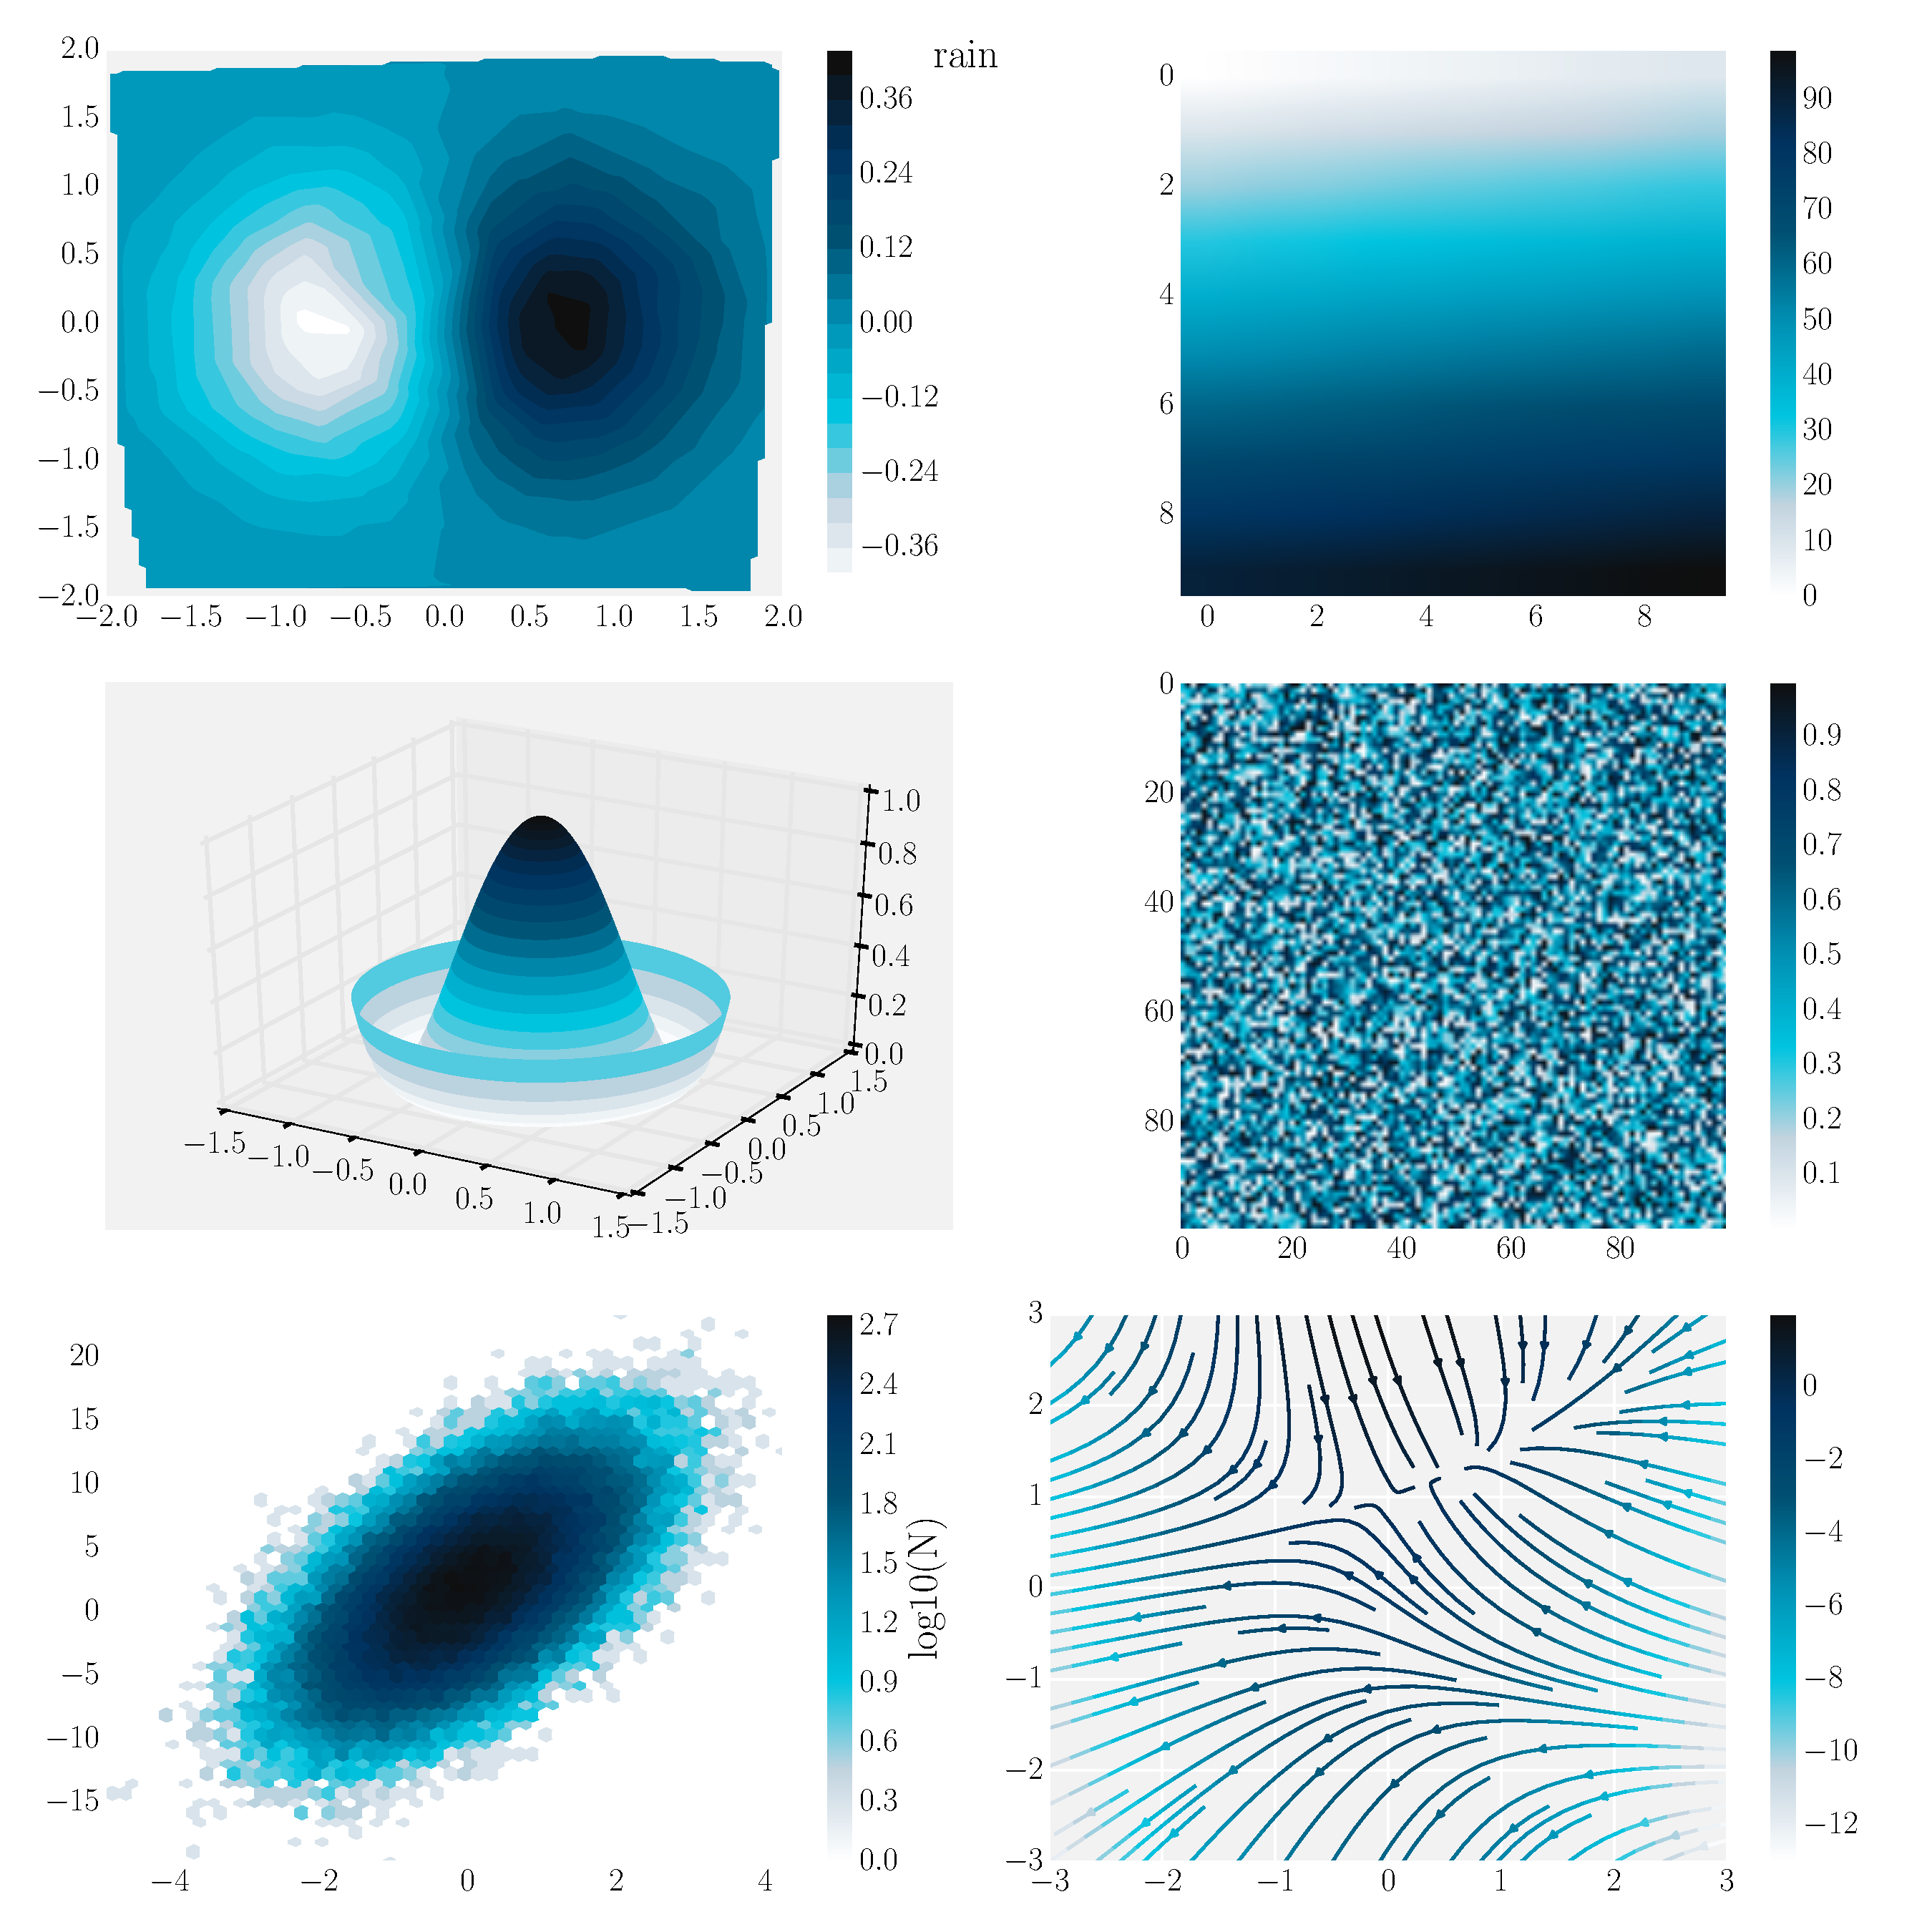
\includegraphics[width=0.99\textwidth]{rainExamples.pdf}
\end{figure}

\newpage
\begin{figure}[ht]
  \centering
  
\includegraphics[width=0.99\textwidth]{seismicBars.pdf}
  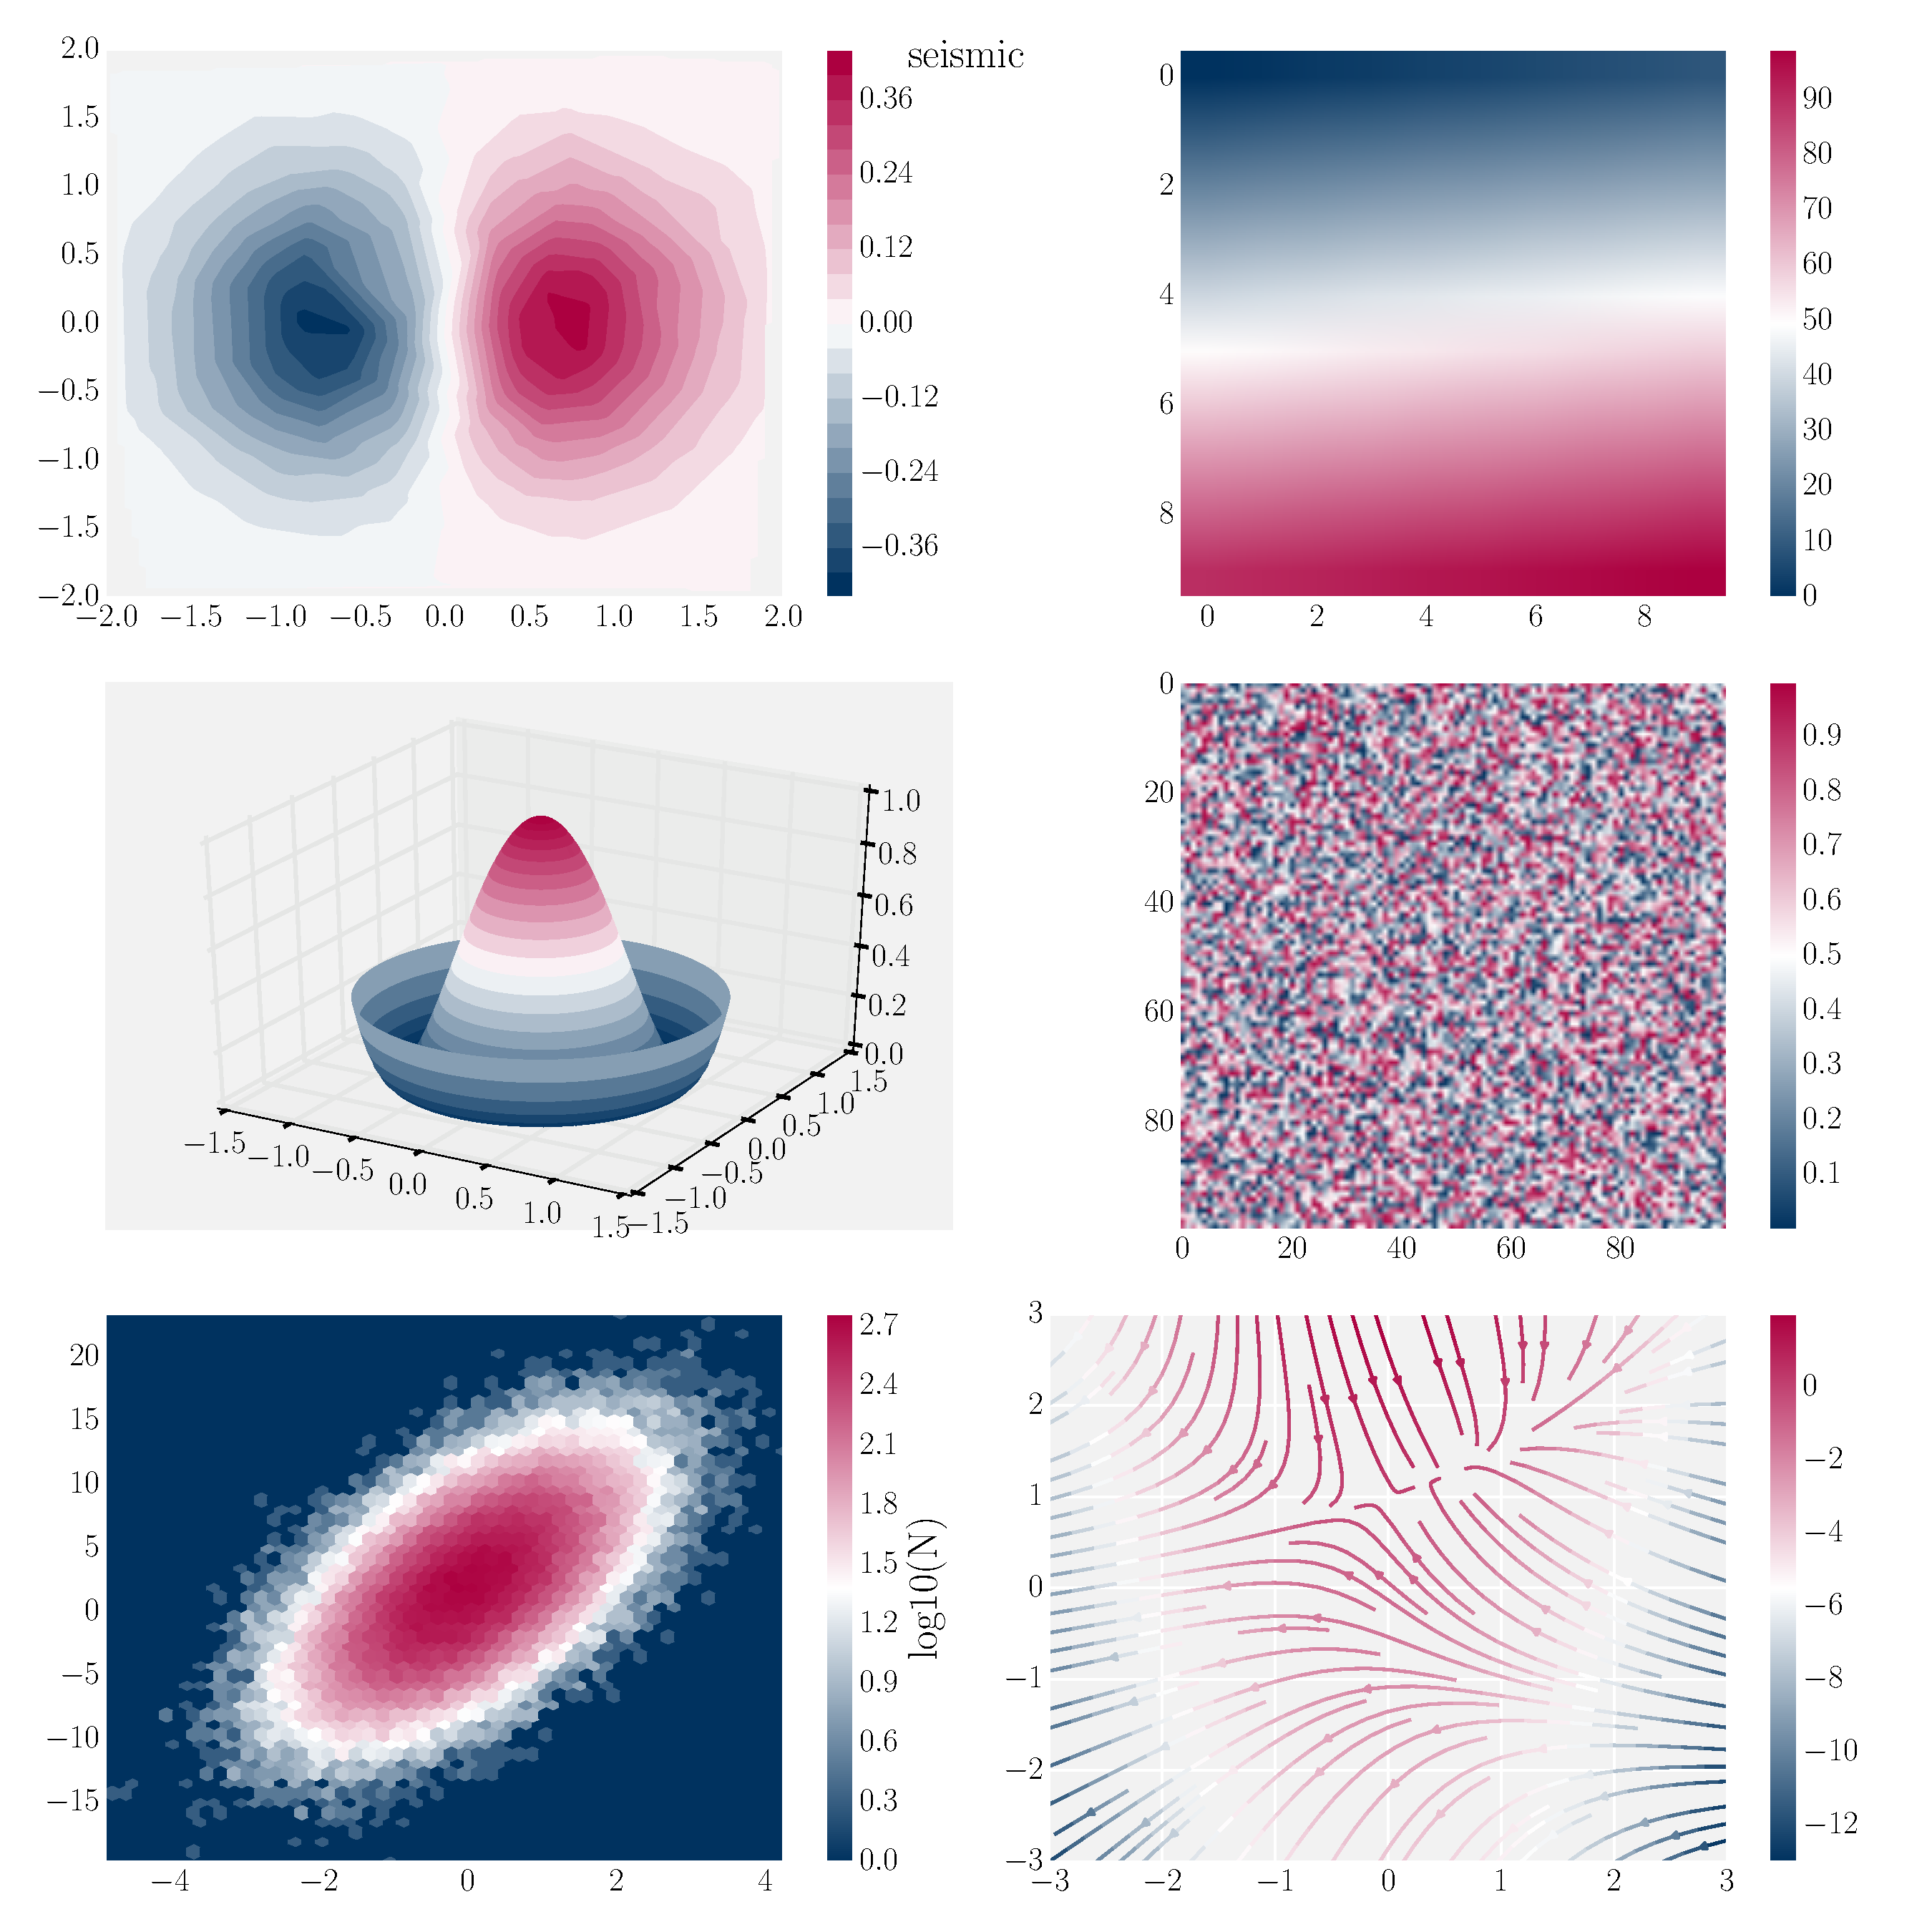
\includegraphics[width=0.99\textwidth]{seismicExamples.pdf}
\end{figure}

\newpage
\begin{figure}[ht]
  \centering
  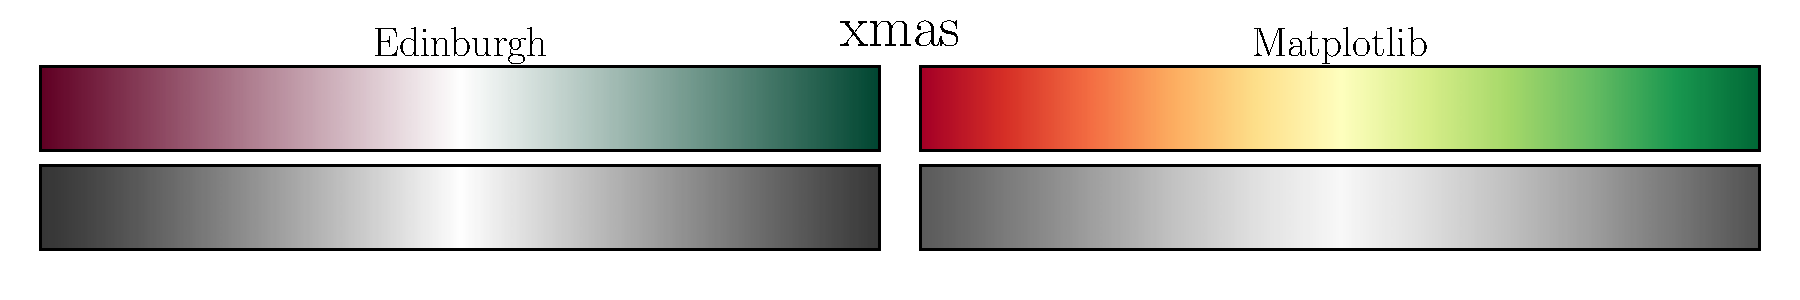
\includegraphics[width=0.99\textwidth]{xmasBars.pdf}
  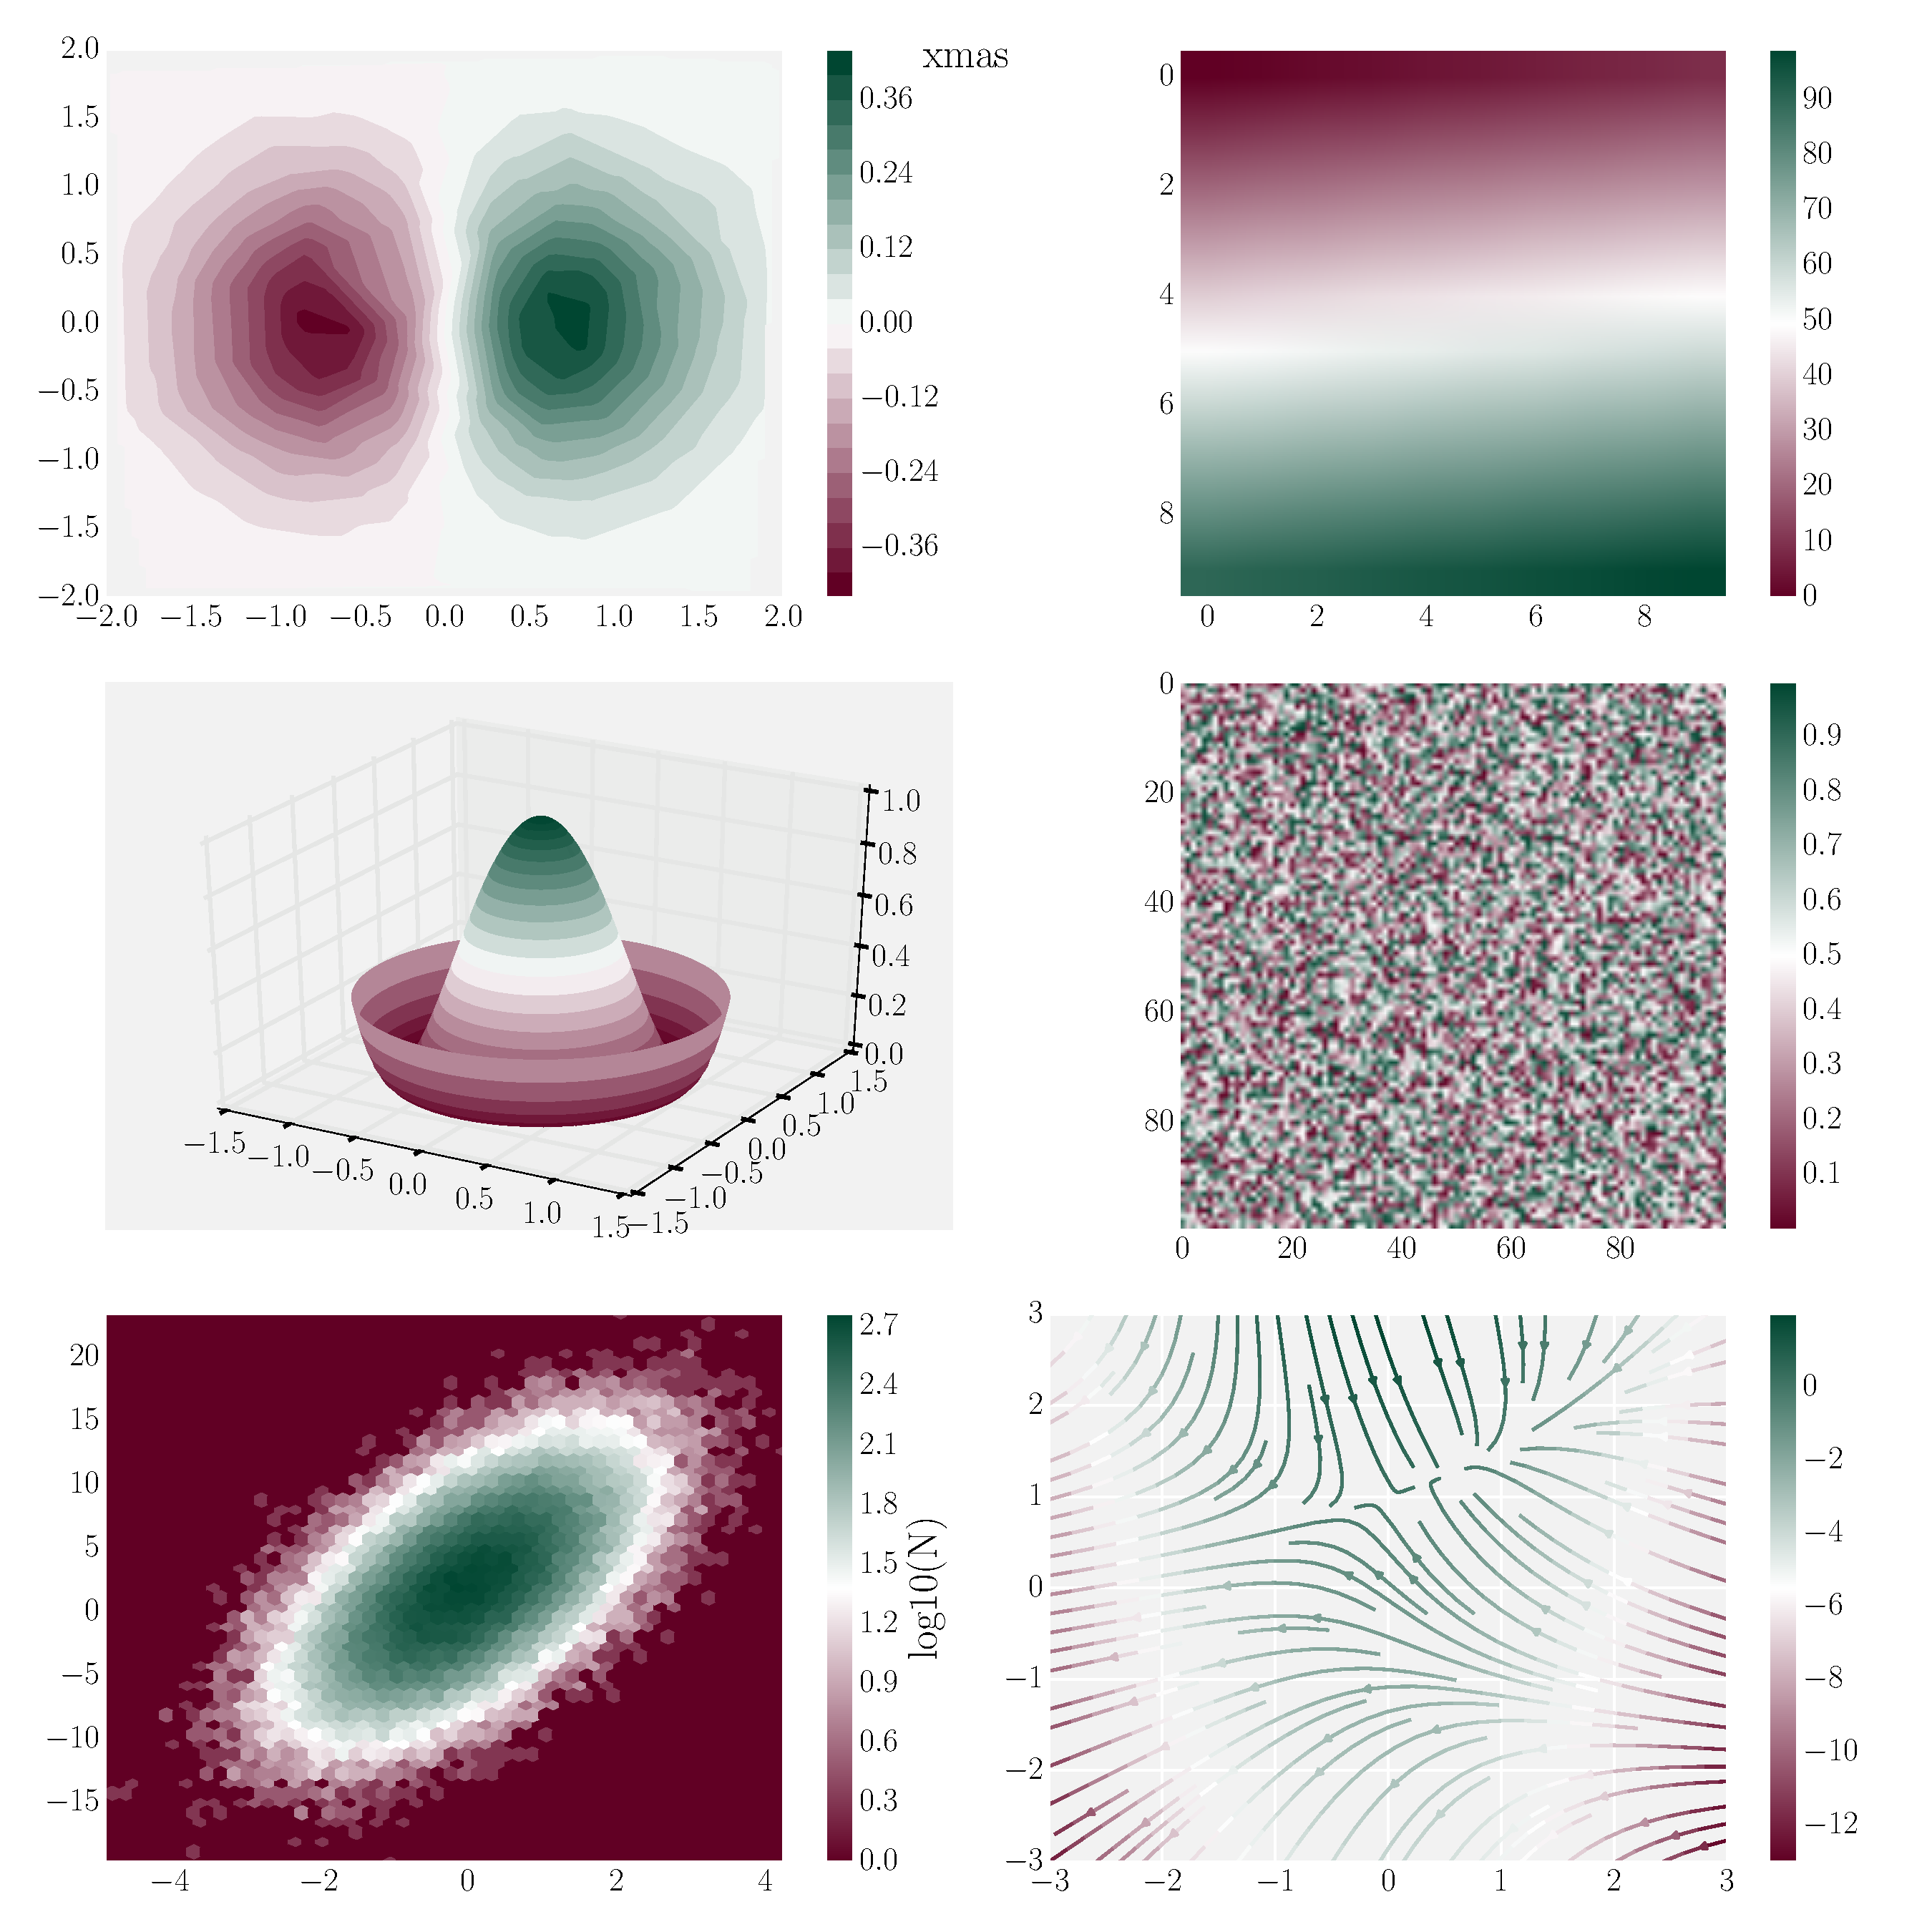
\includegraphics[width=0.99\textwidth]{xmasExamples.pdf}
\end{figure}

\newpage
\begin{figure}[ht]
  \centering
  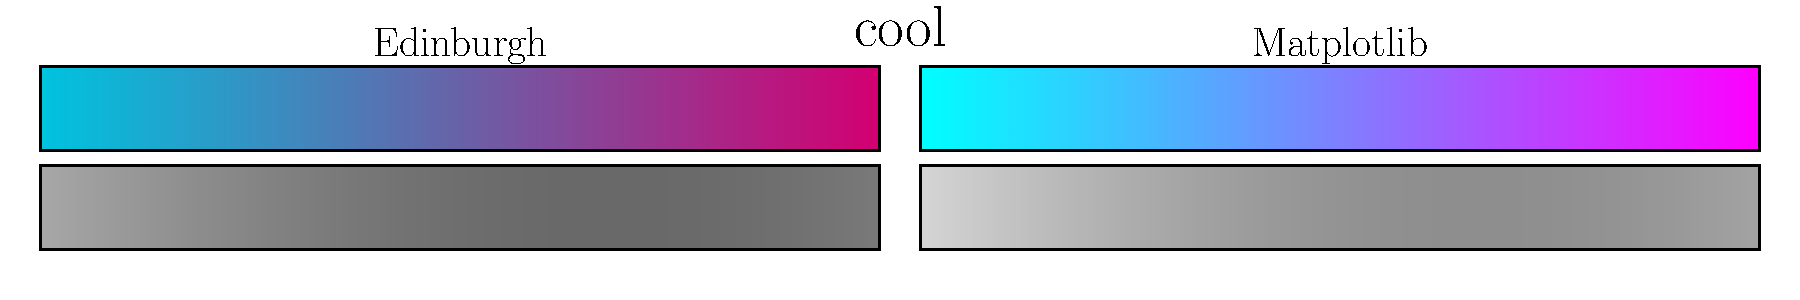
\includegraphics[width=0.99\textwidth]{coolBars.pdf}
  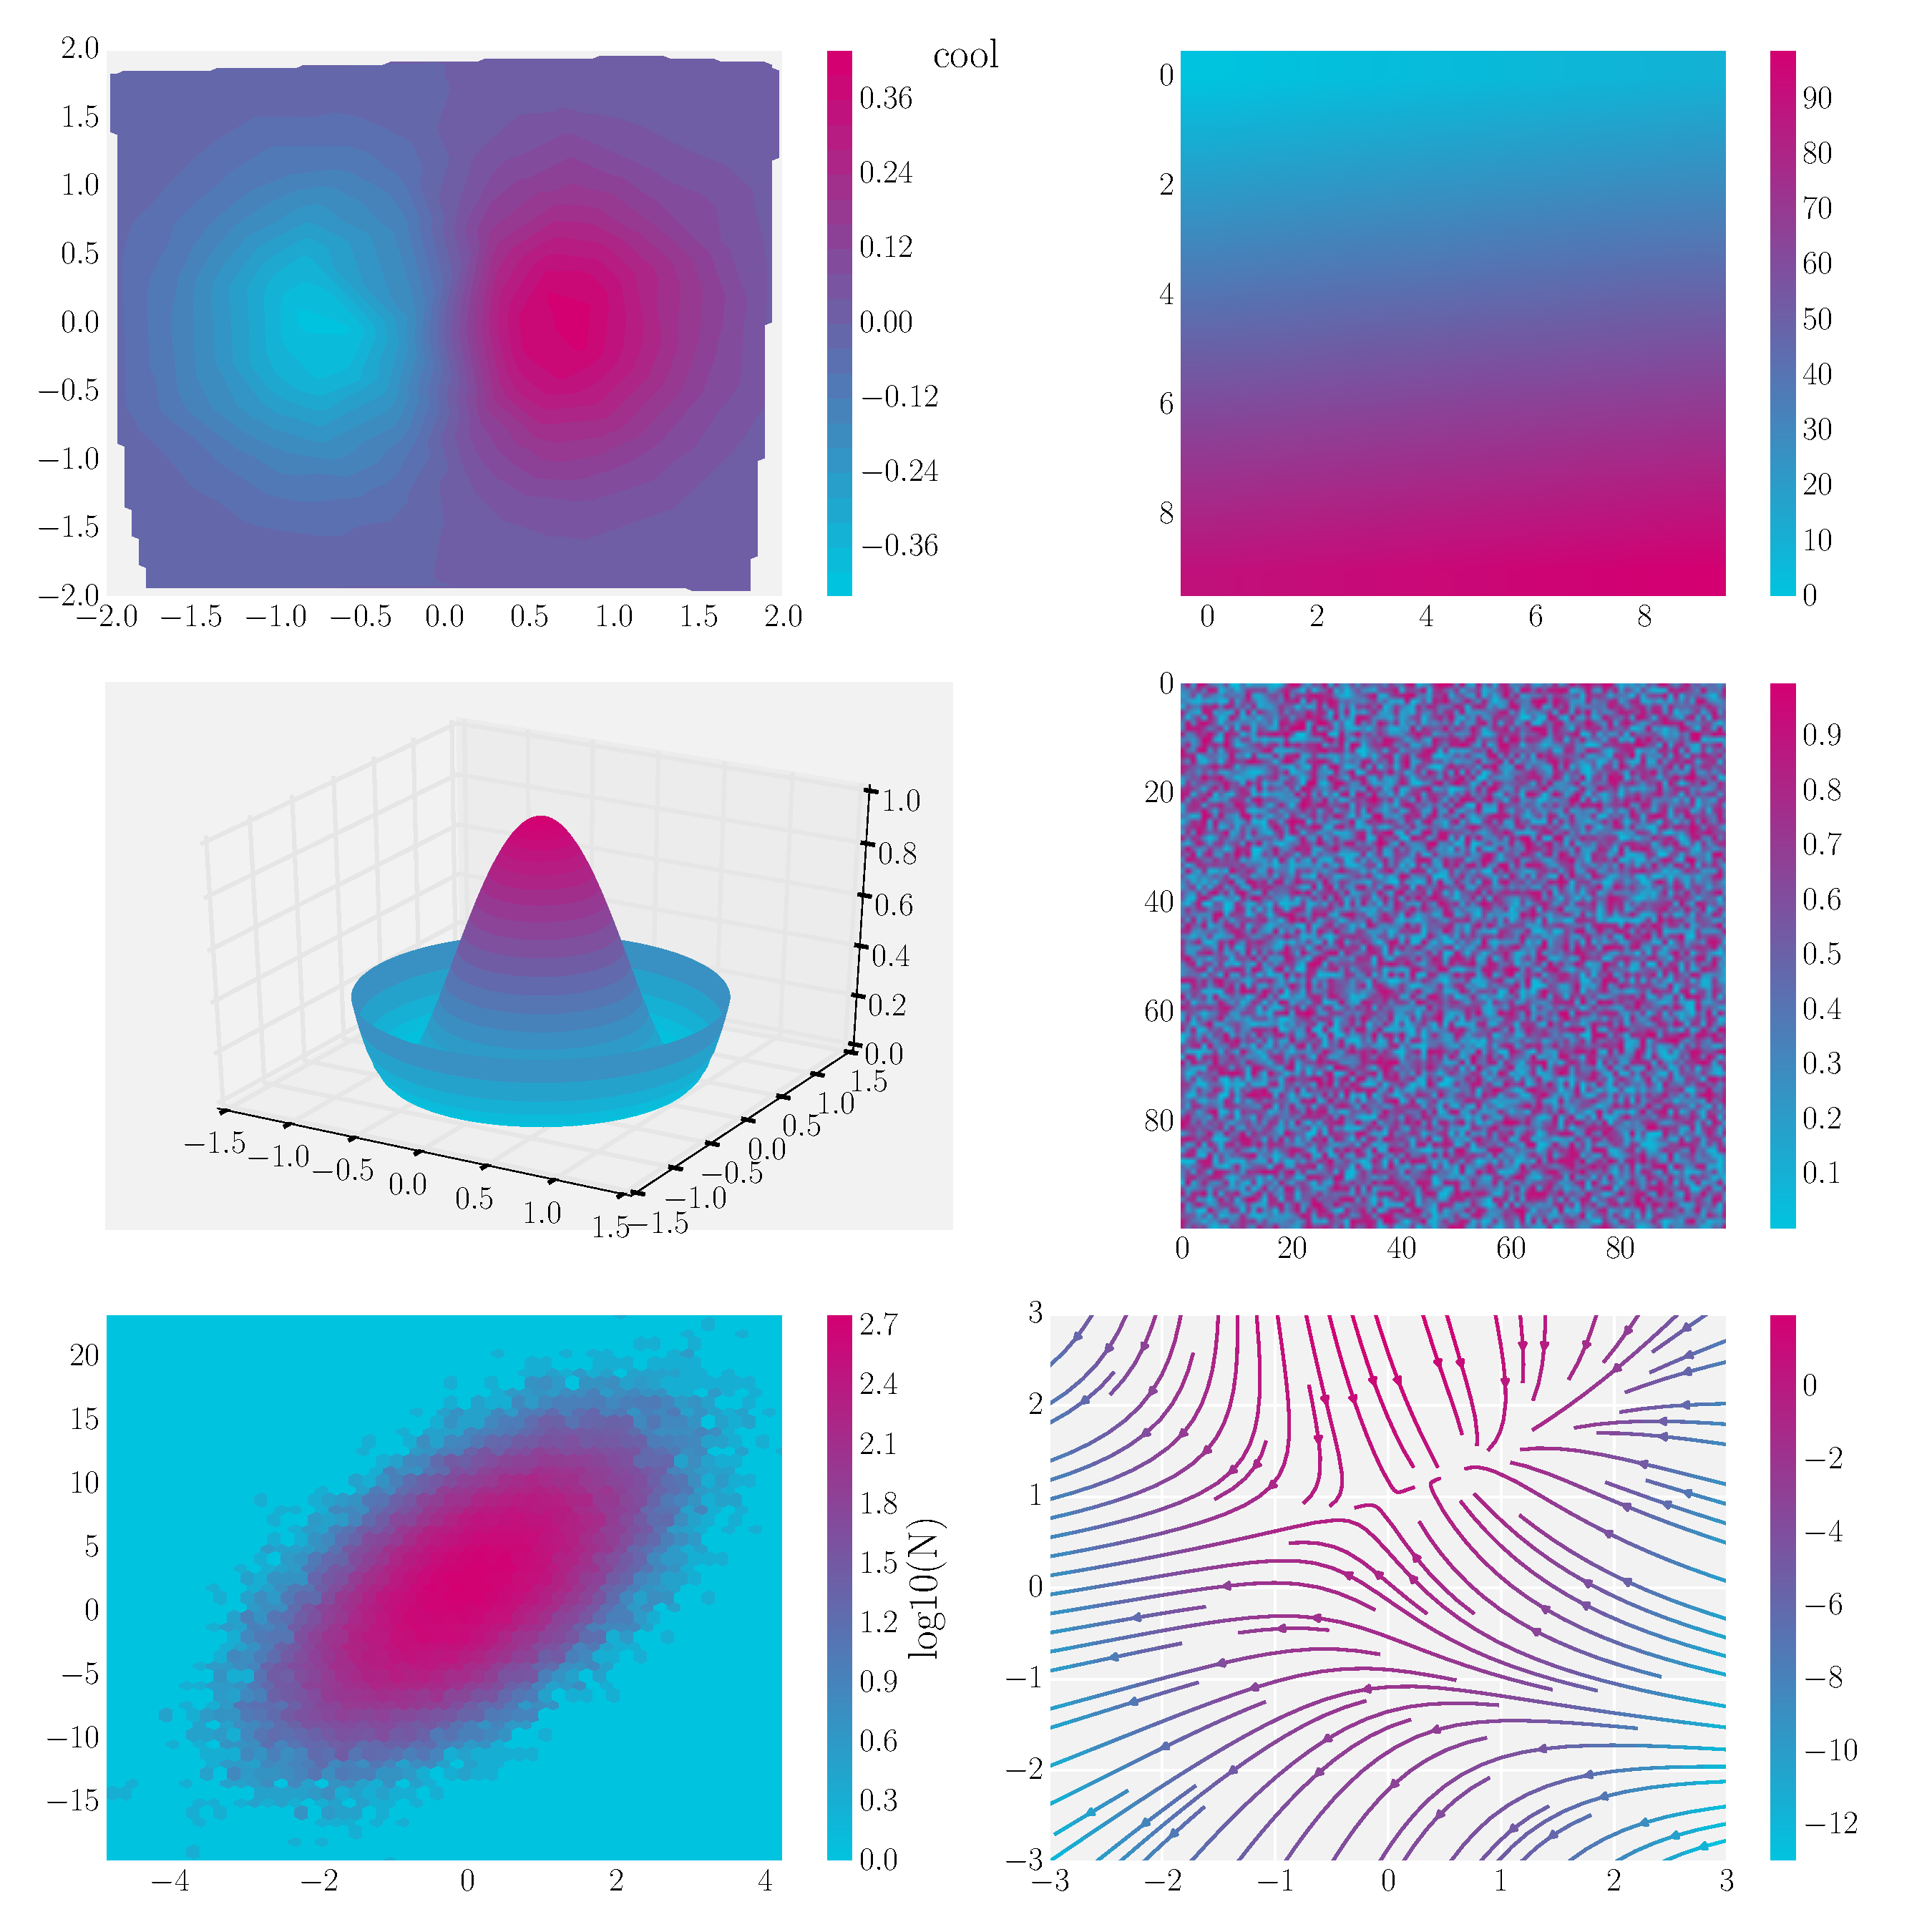
\includegraphics[width=0.99\textwidth]{coolExamples.pdf}
\end{figure}

\newpage
\begin{figure}[ht]
  \centering
  
\includegraphics[width=0.99\textwidth]{deepseaBars.pdf}
  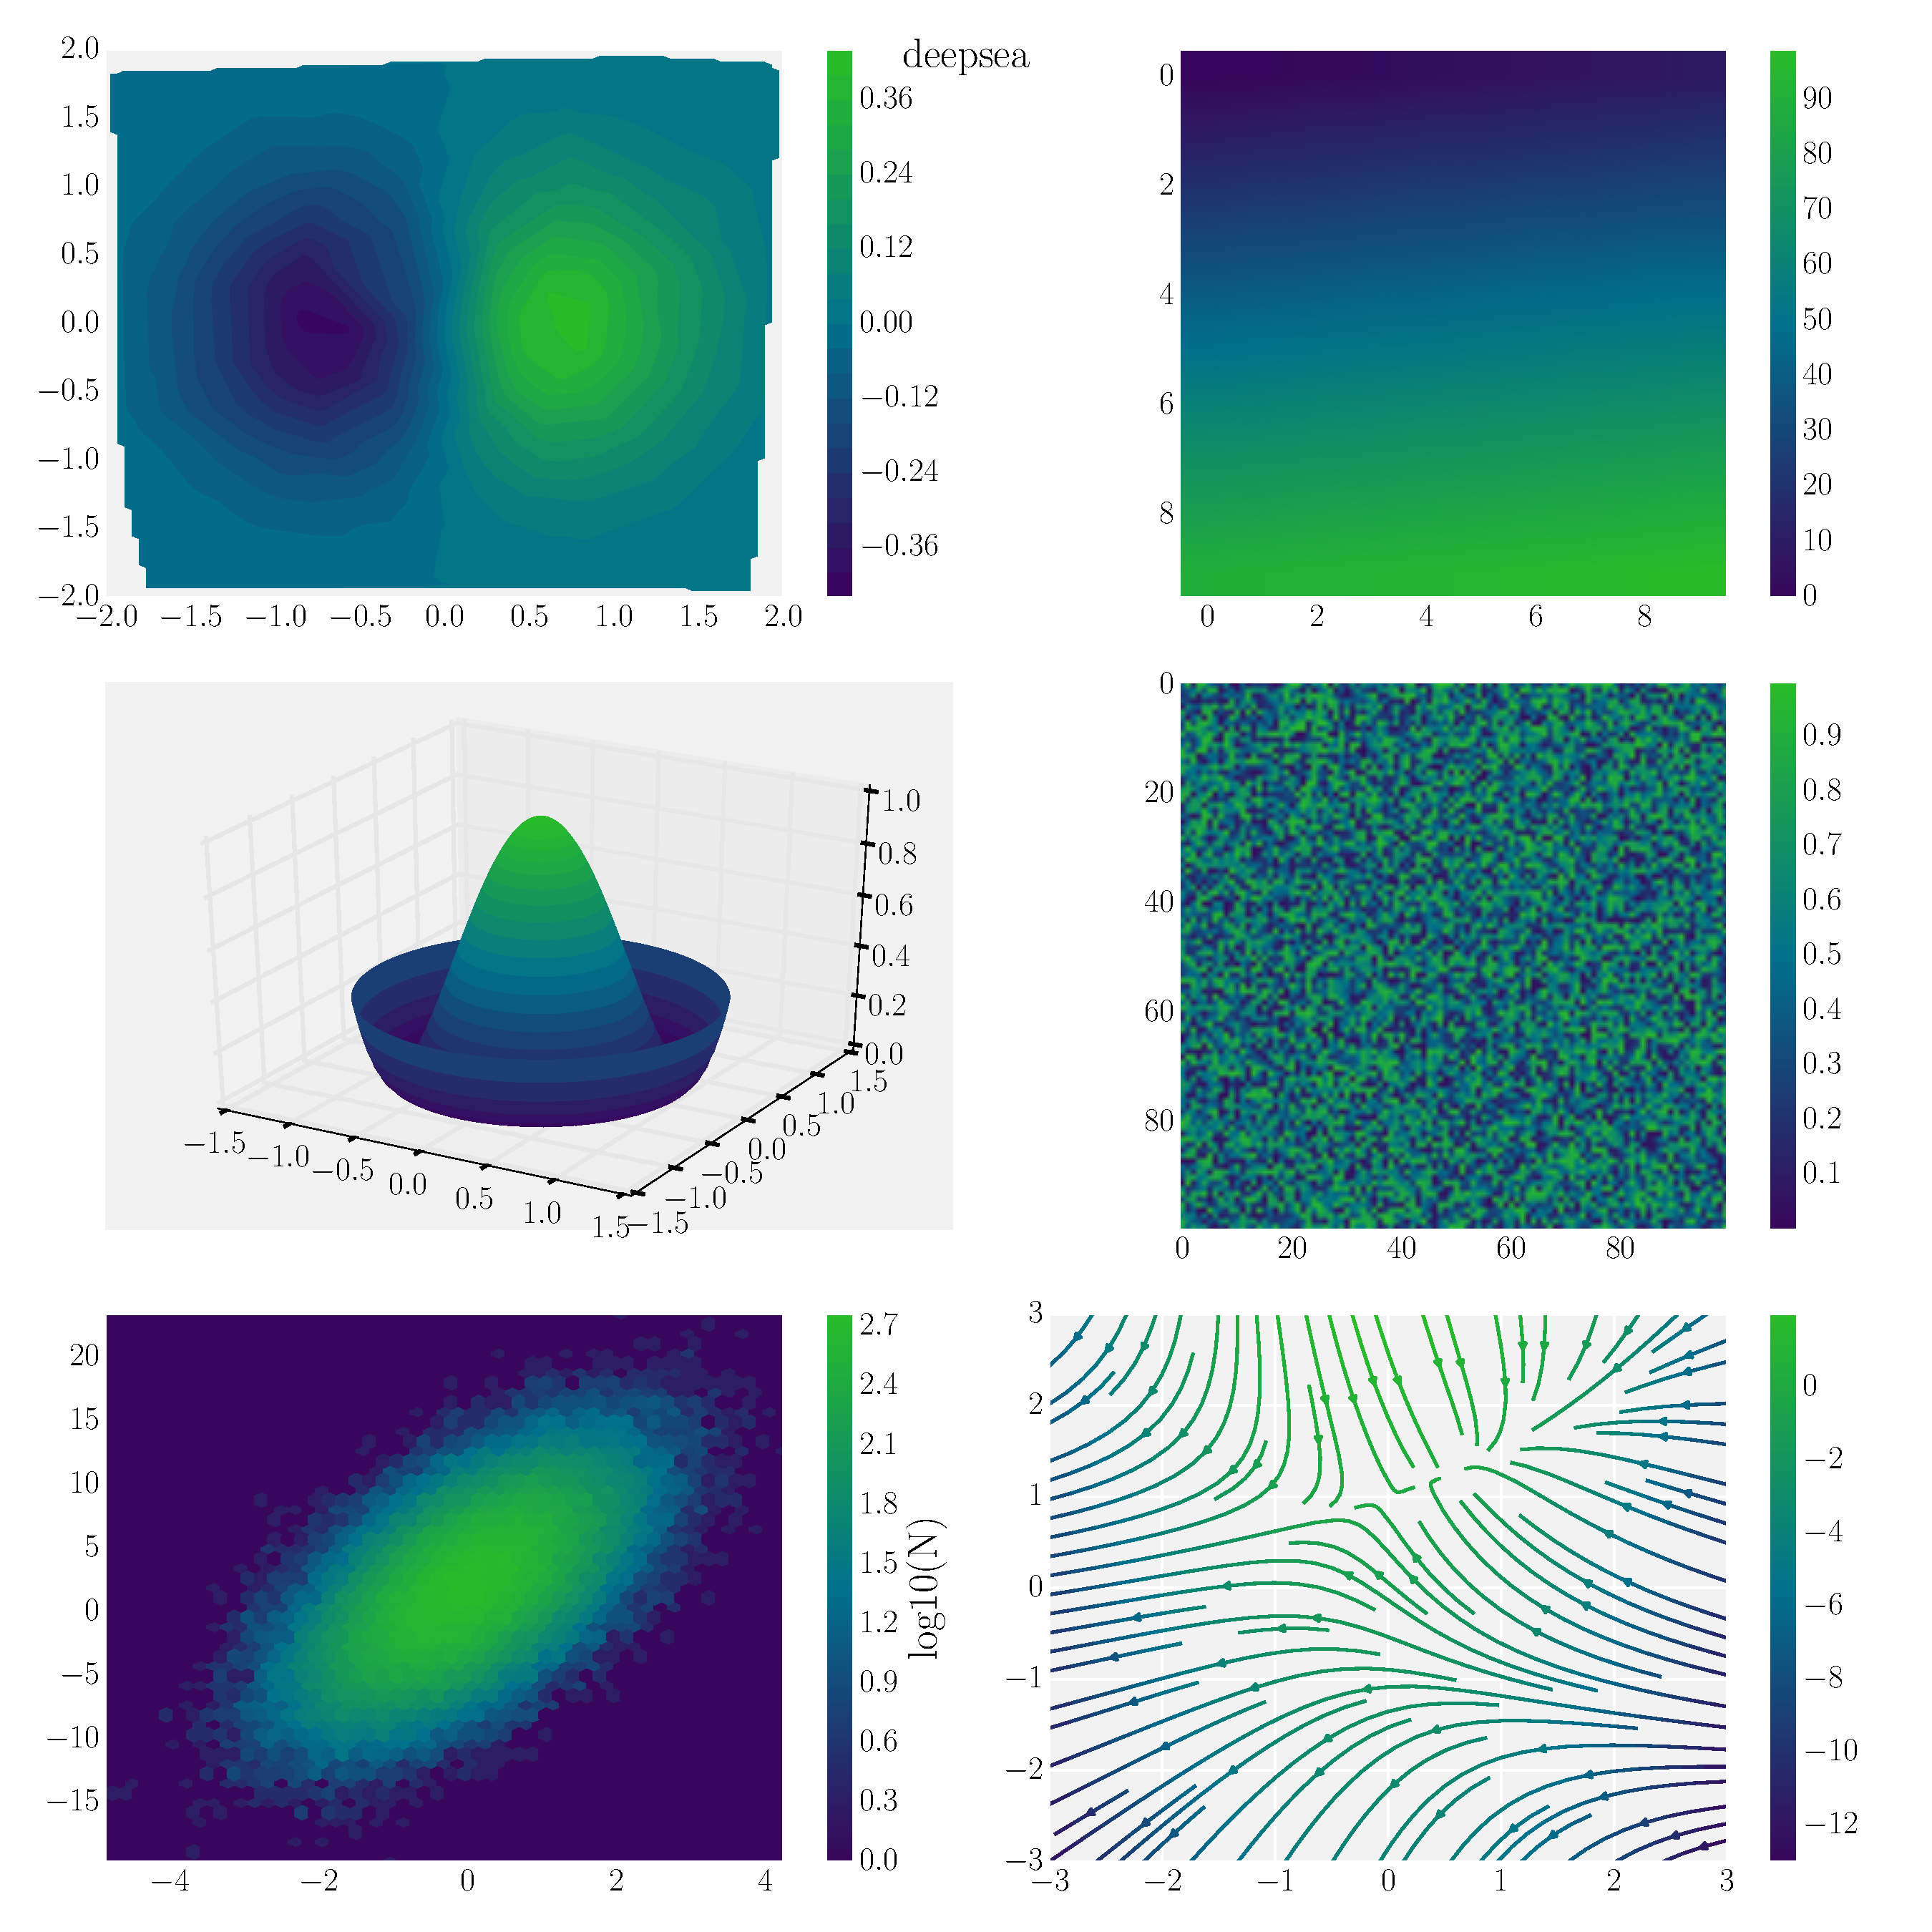
\includegraphics[width=0.99\textwidth]{deepseaExamples.pdf}
\end{figure}



% 
% \pagebreak
% 
% Now the five that I suggest we reject.
% 
% \begin{figure}[ht]
%   \centering
%   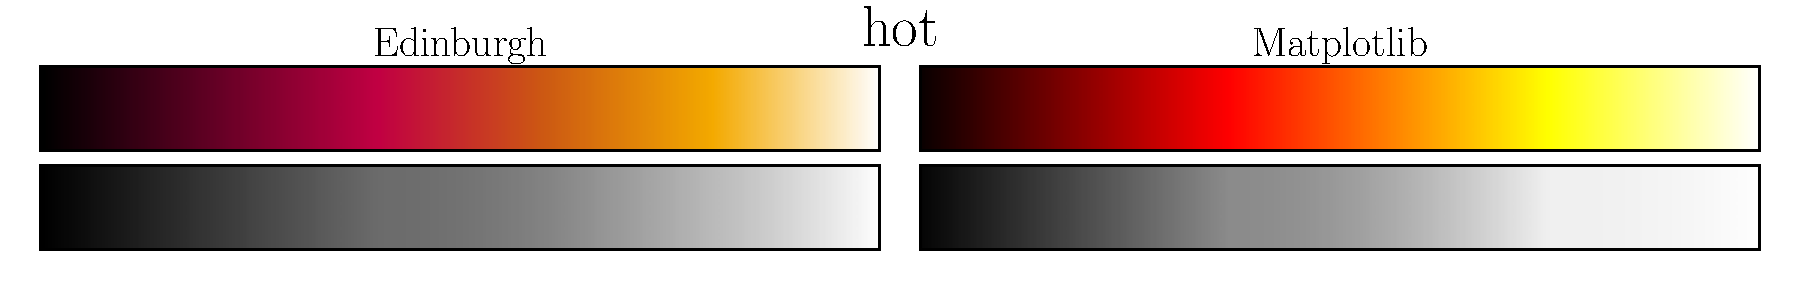
\includegraphics[width=0.45\textwidth]{hotBars.pdf}
%   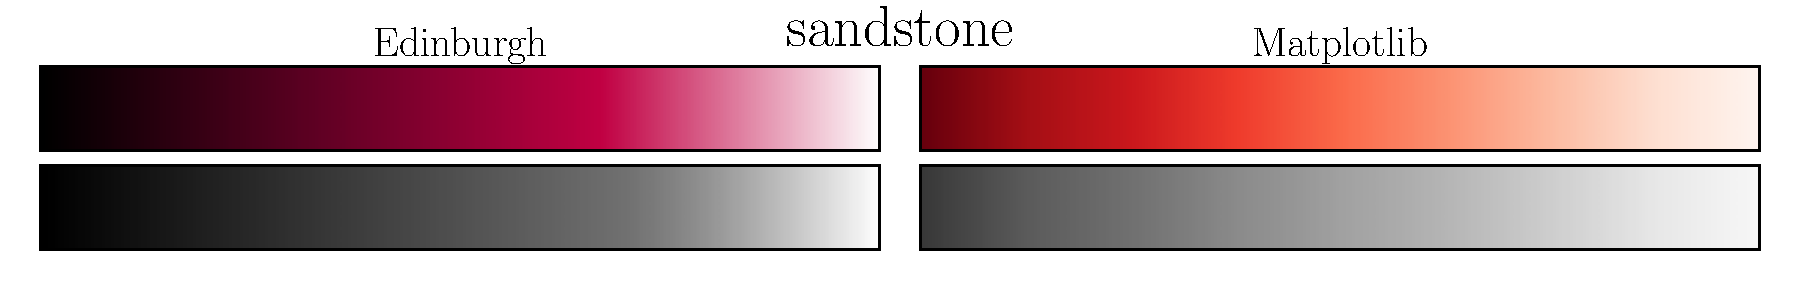
\includegraphics[width=0.45\textwidth]{cherryBars.pdf}
%   \\
%   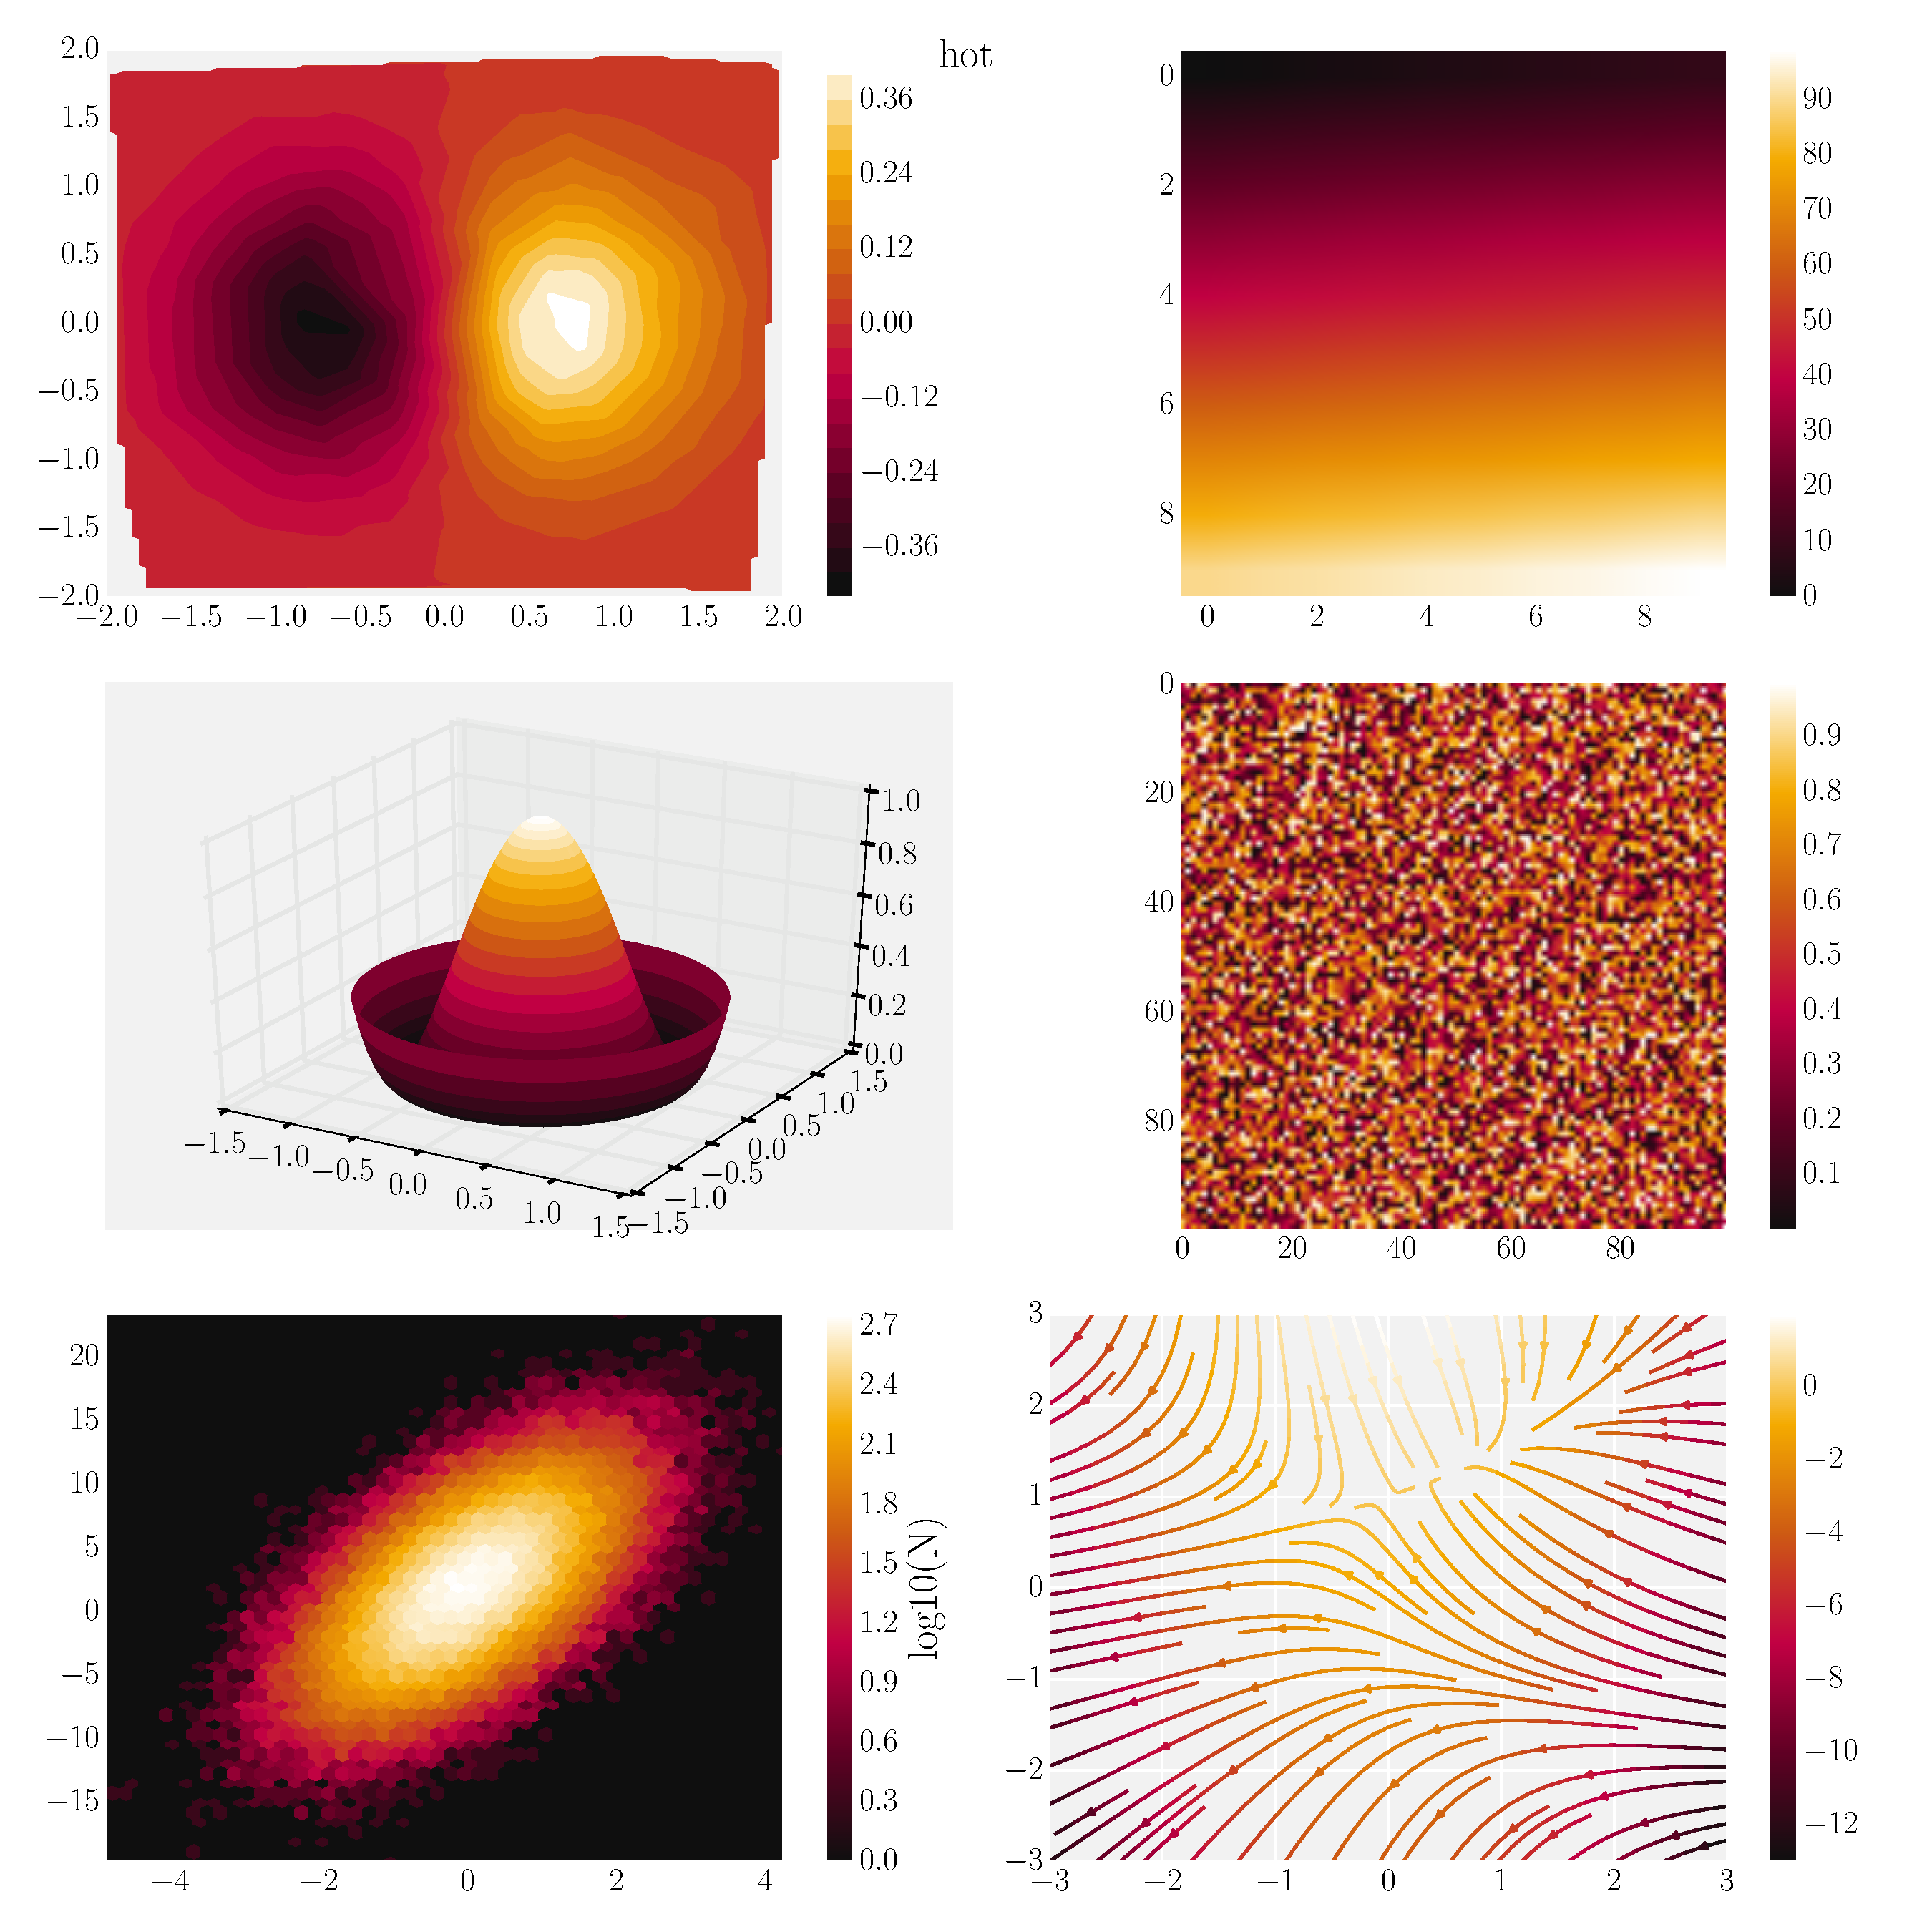
\includegraphics[width=0.45\textwidth]{hotExamples.pdf}
%   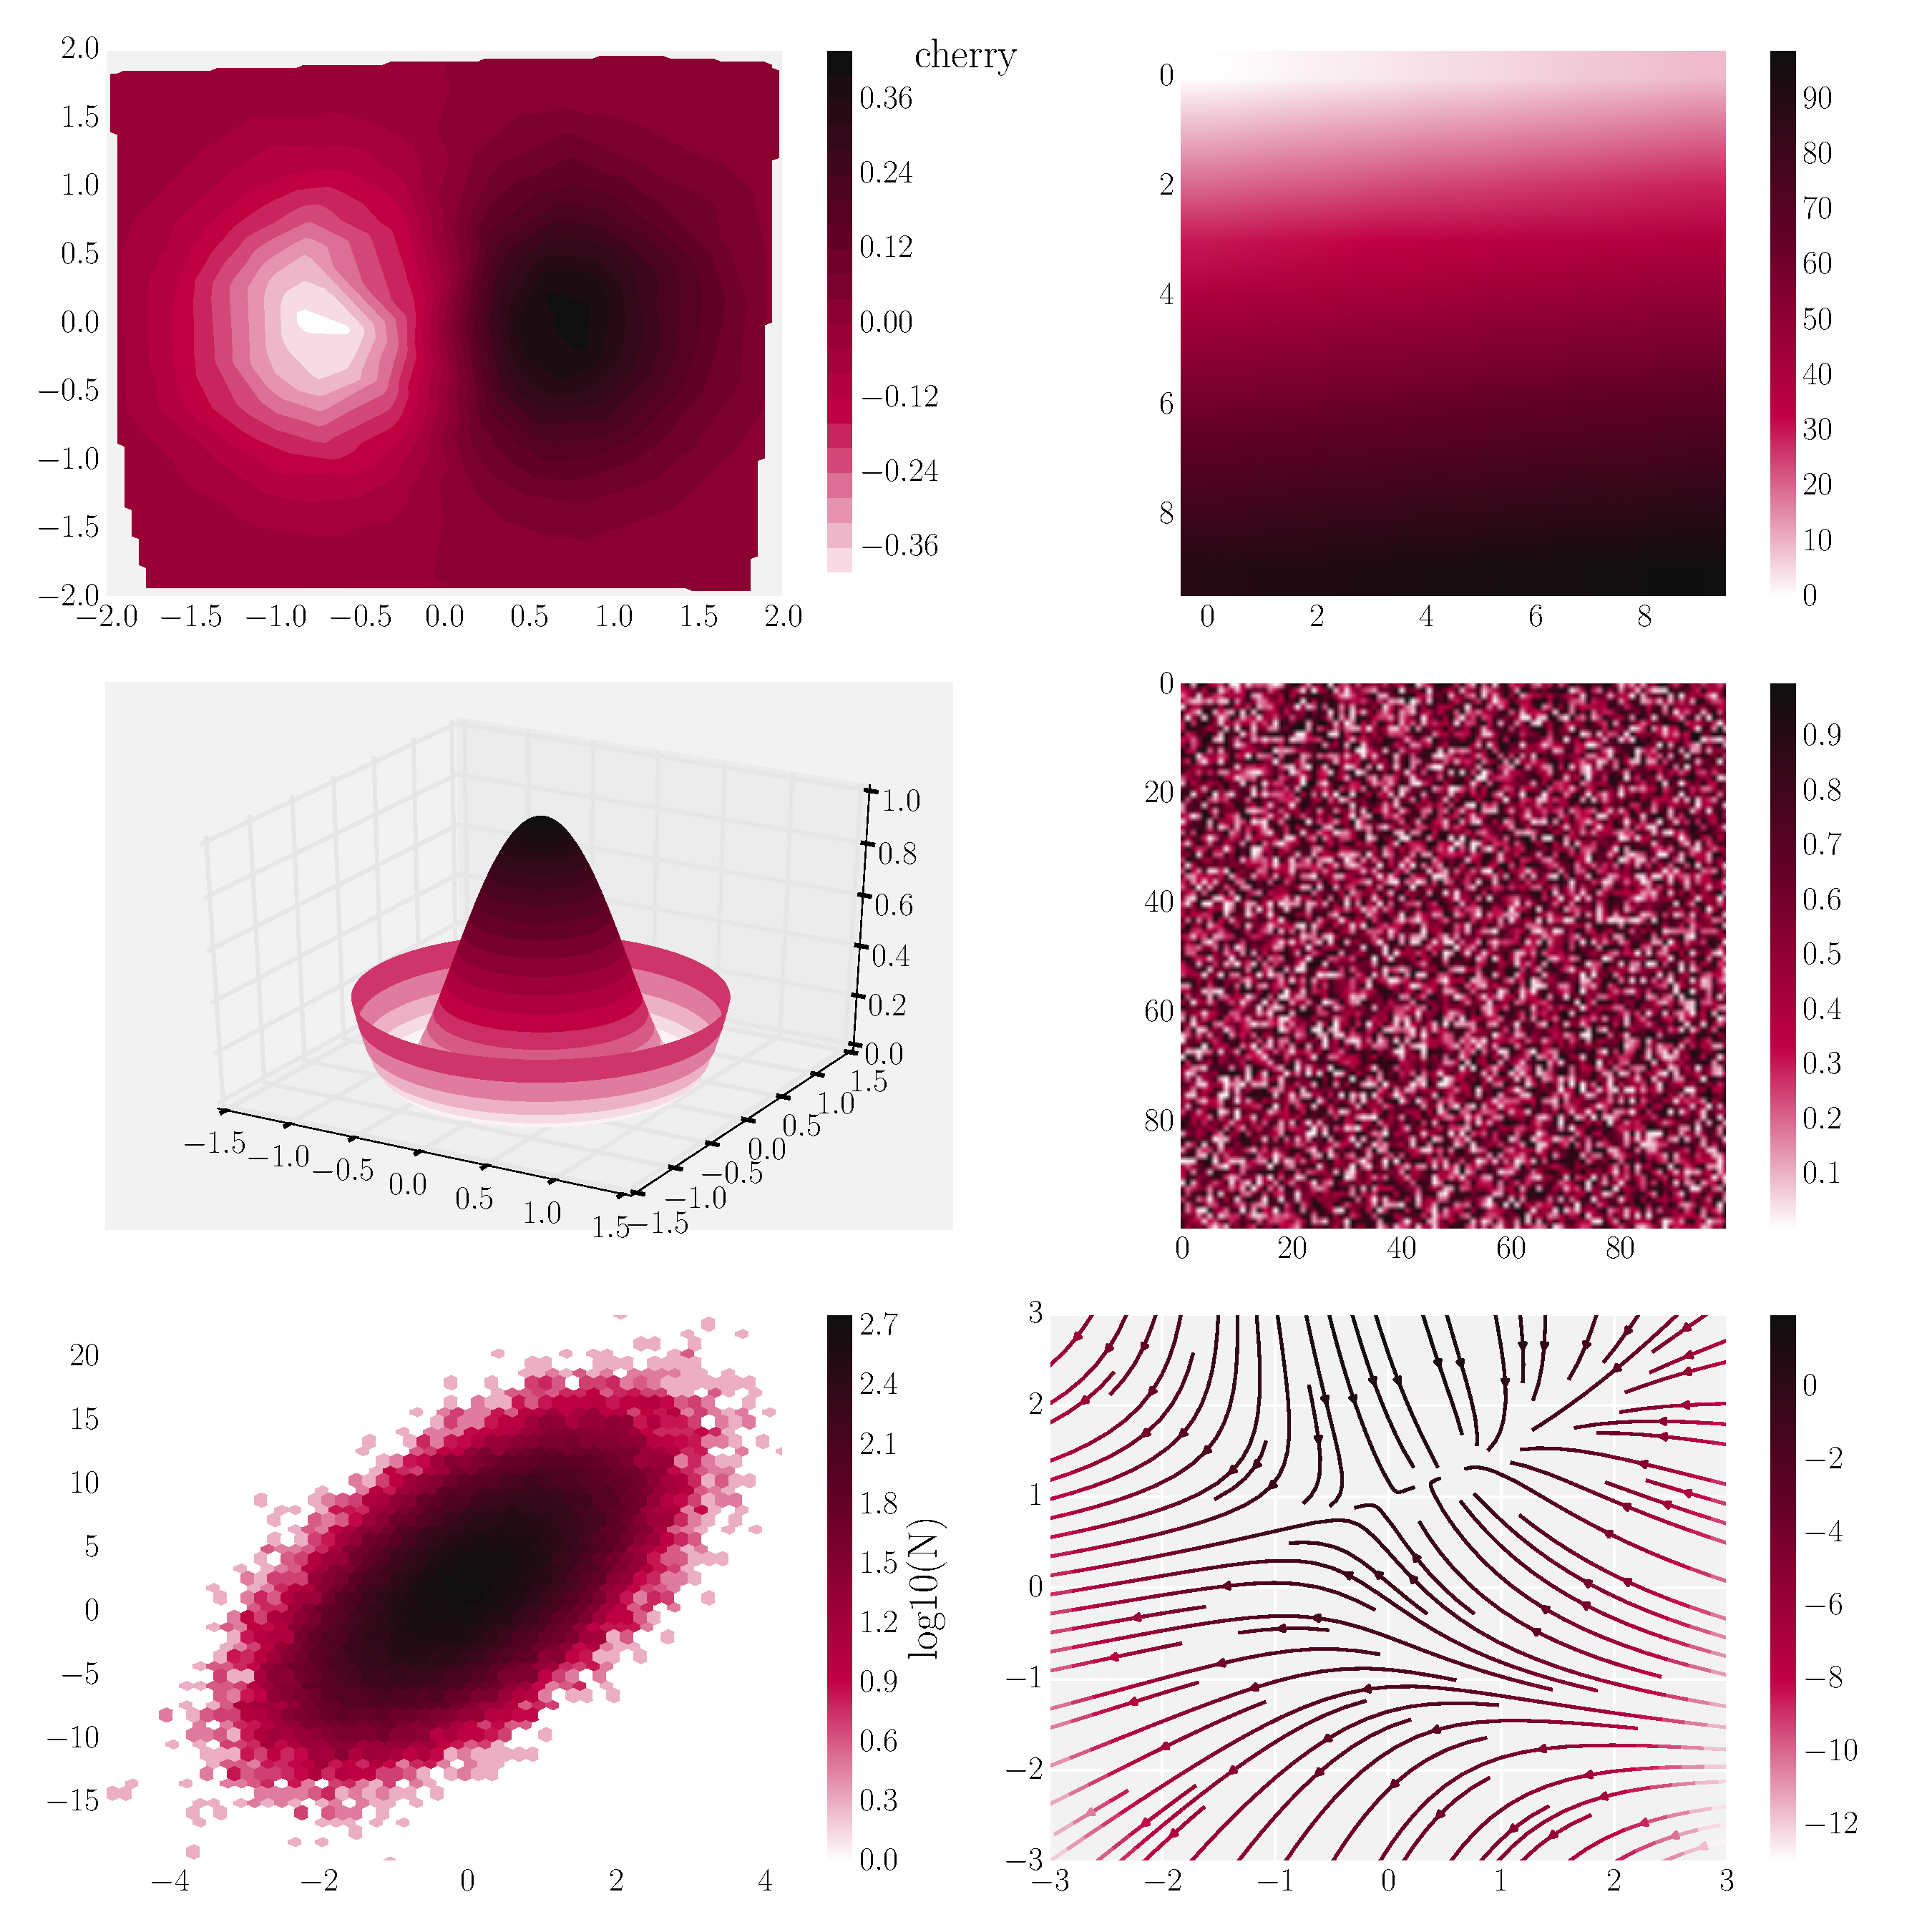
\includegraphics[width=0.45\textwidth]{cherryExamples.pdf}
% \end{figure}
% 
% \begin{figure}[ht]
%   \centering
%   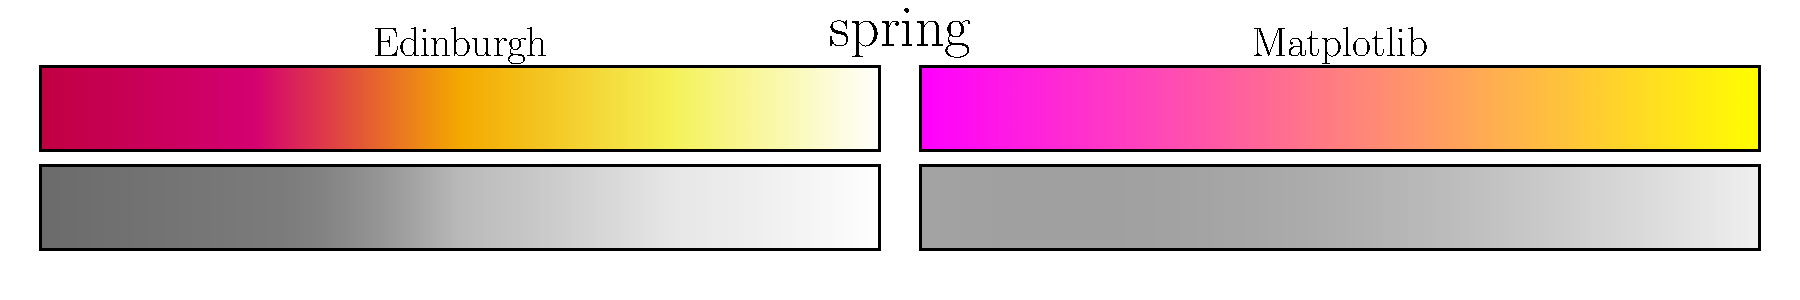
\includegraphics[width=0.45\textwidth]{springBars.pdf}
%   
\includegraphics[width=0.45\textwidth]{bombpopsBars.pdf}
%   \\
%   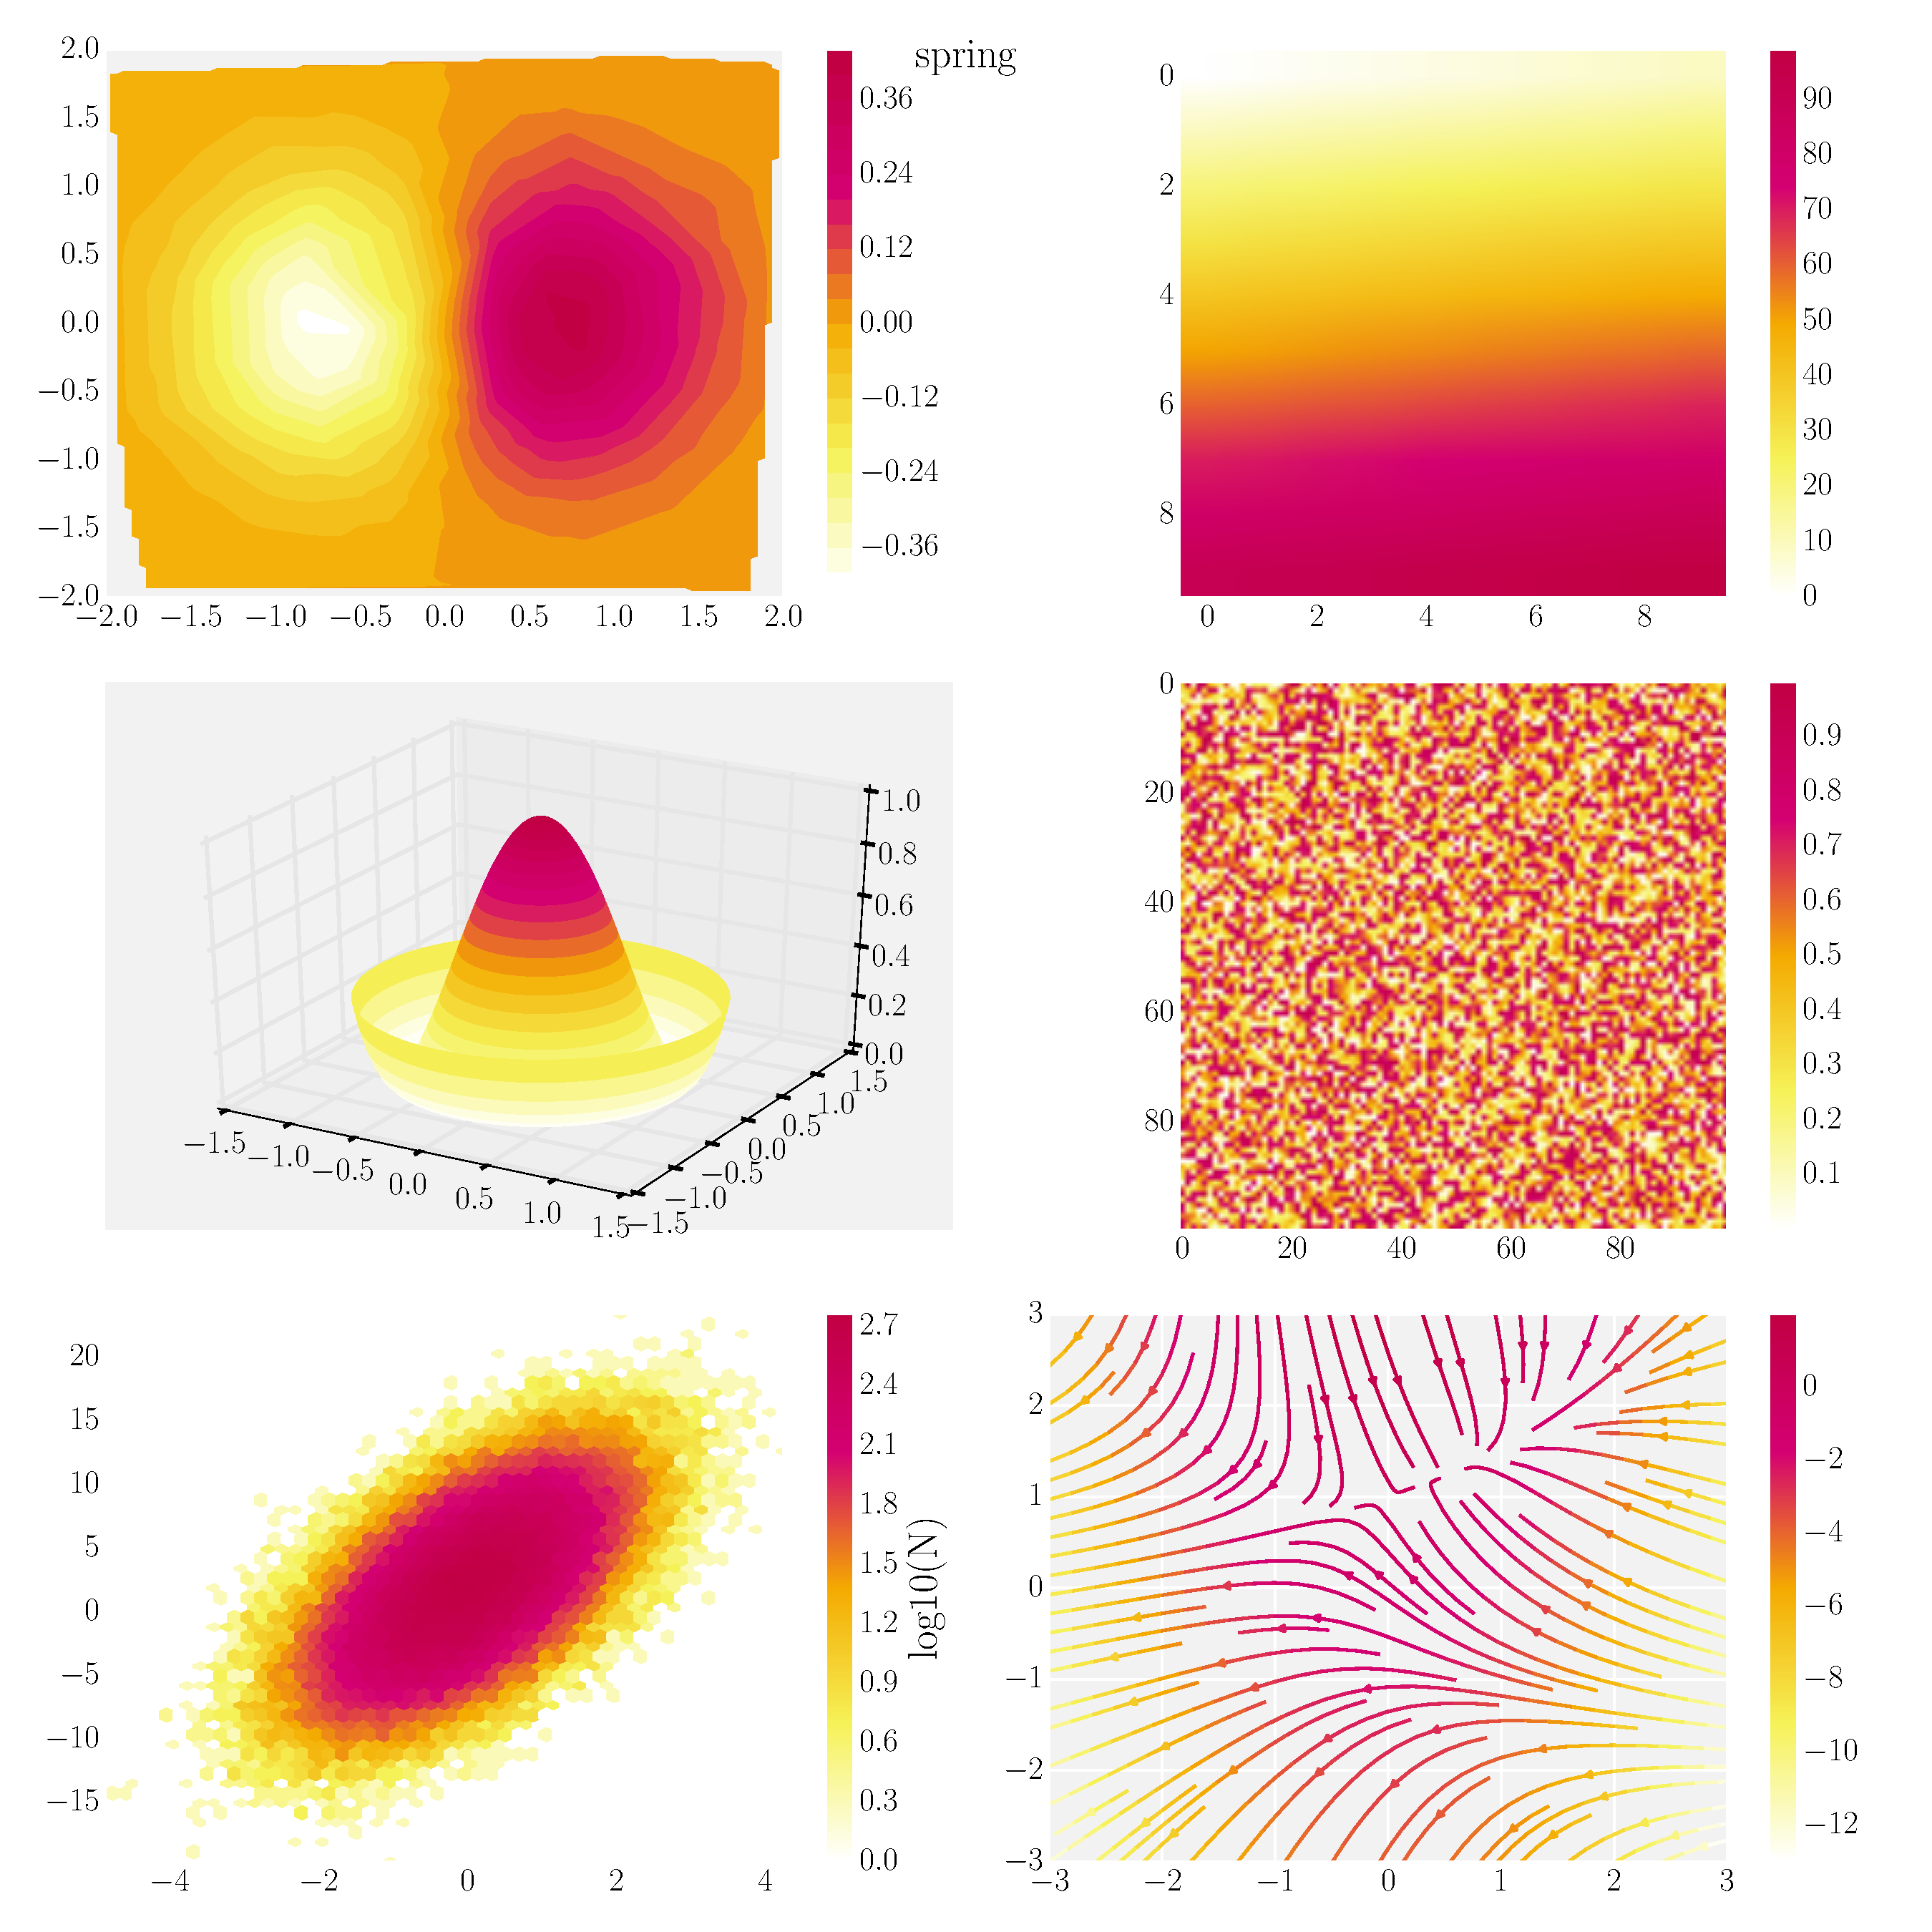
\includegraphics[width=0.45\textwidth]{springExamples.pdf}
%   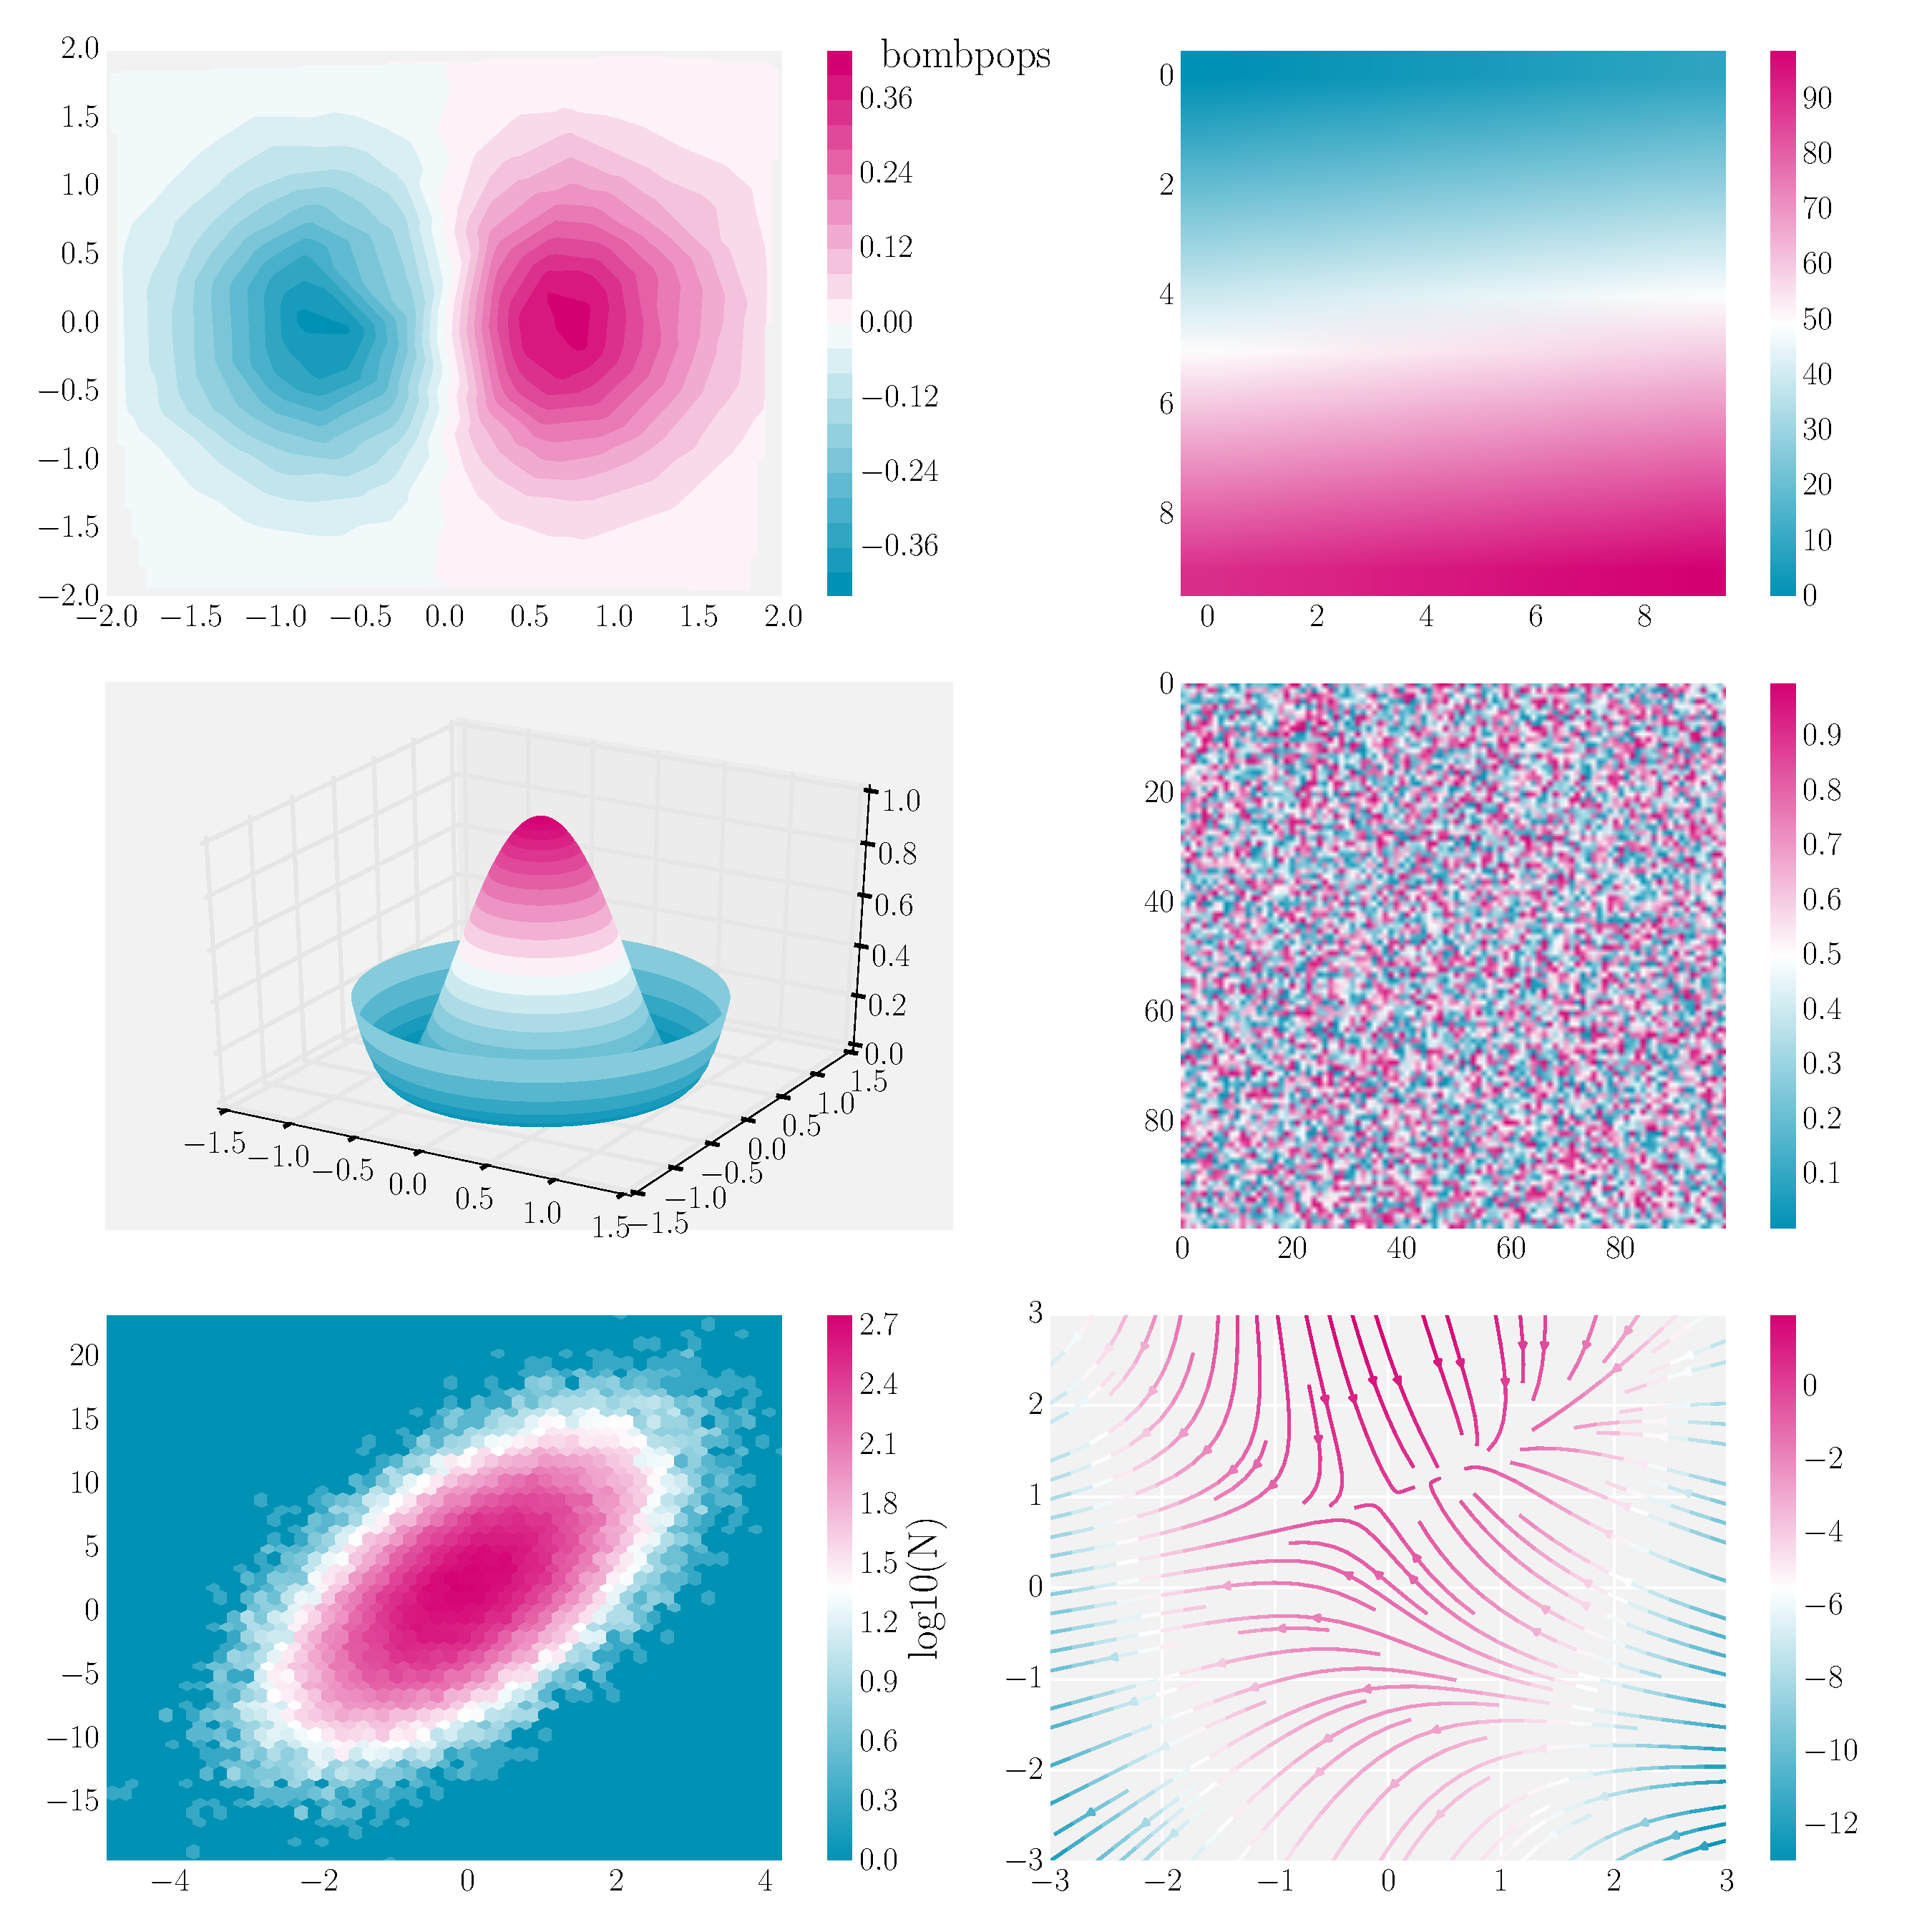
\includegraphics[width=0.45\textwidth]{bombpopsExamples.pdf}
% \end{figure}
% 
% \begin{figure}[h]
%   \centering
%   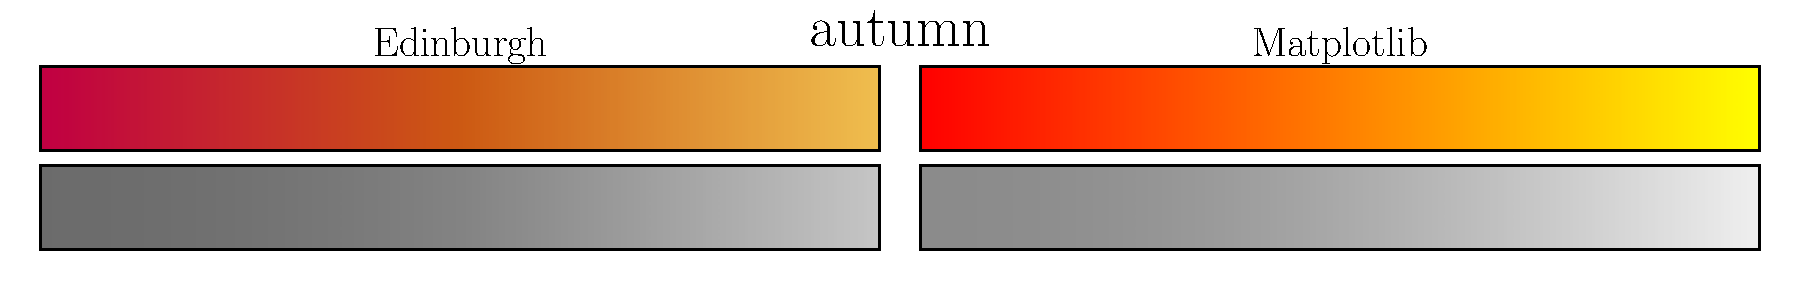
\includegraphics[width=0.45\textwidth]{autumnBars.pdf}\\
%   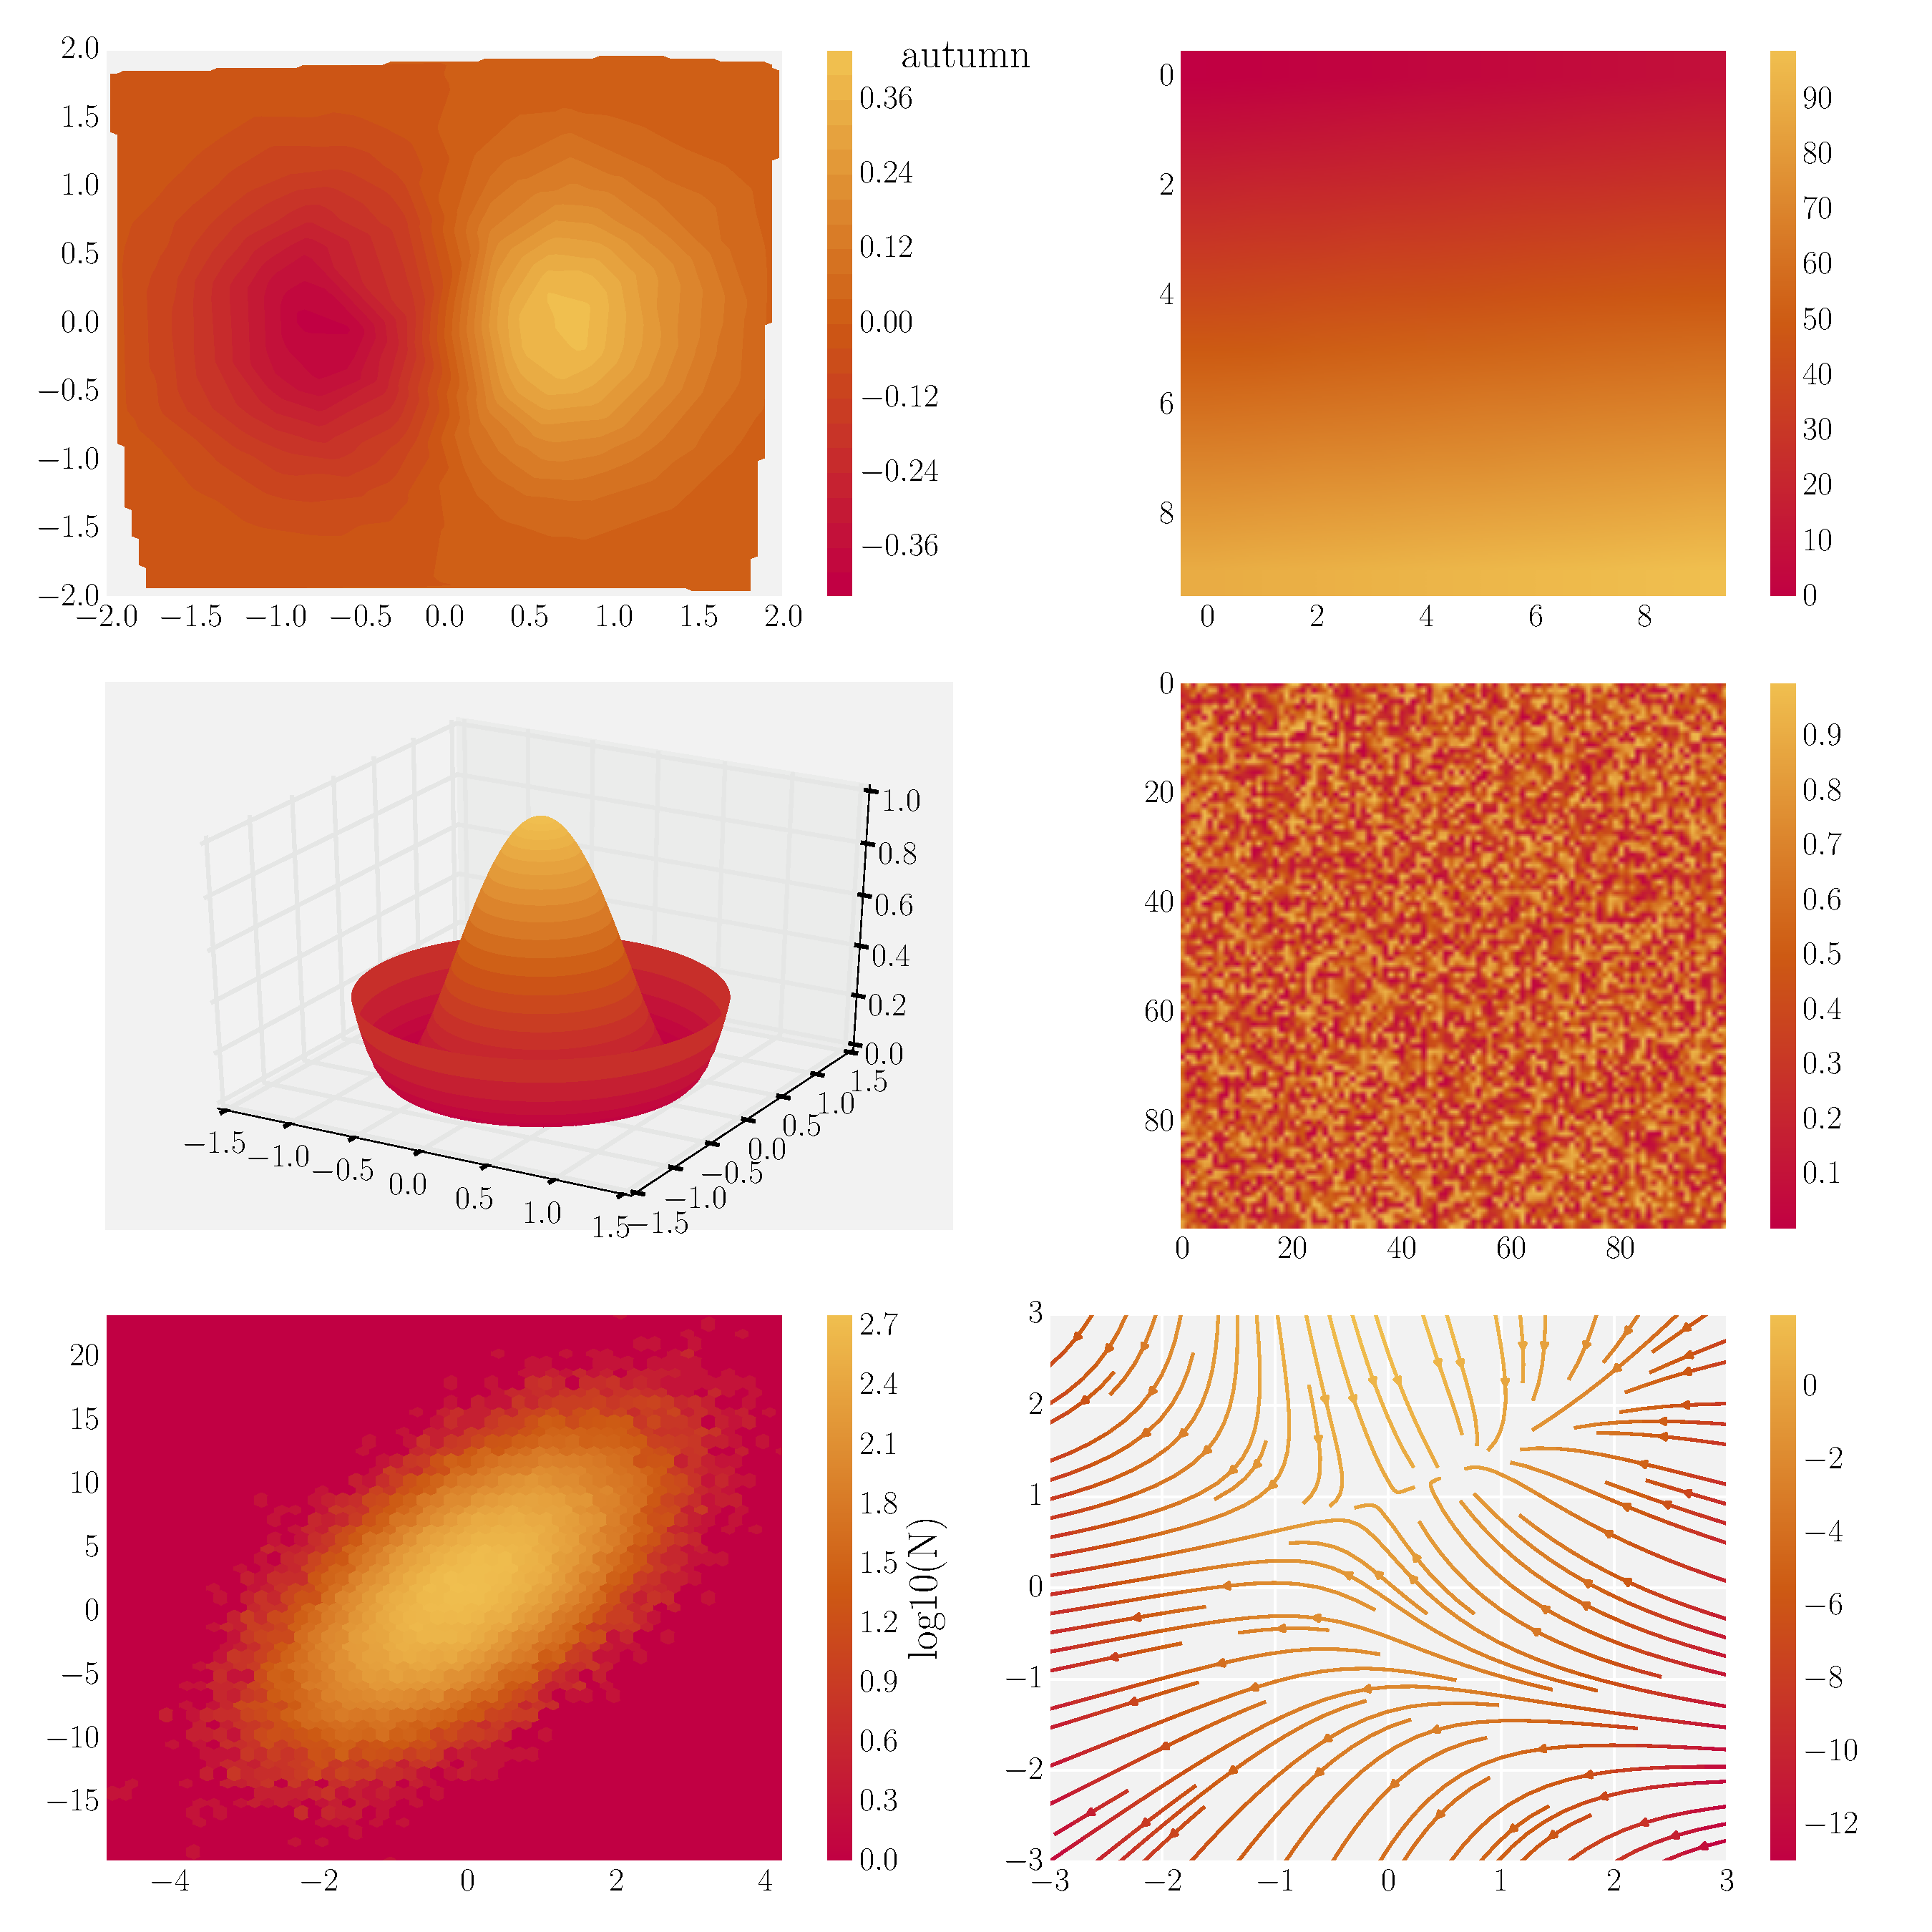
\includegraphics[width=0.45\textwidth]{autumnExamples.pdf}
% \end{figure}


\end{document}
